%%%%%%%%%%%%%%%%%%%%%%%%%%%%%%%%%%%%%%%%%%%%%%%%%%%%%%%%%%%%%%%%%%%%%%%%%%%%%%%%%%%%%%%%%%%%%%%%%%%%%%%%%%%
\chapter{Statistics}\label{S:Statistics}

\section{Data and Statistics}\label{S:DataStats}

\begin{definition}[Data]
The function $X$ measures the outcome $\omega$ of an experiment with sample space $\Omega$ [Often, the sample space is also denoted by $S$].  Formally, $X$ is a random variable [or a random vector $X=(X_1,X_2,\ldots,X_n)$, i.e.~a vector of random variables] taking  values in the {\bf data space} $\Xz$:
\[
X(\omega):\Omega \to \Xz \ .
\]
The realisation of the RV $X$ when an experiment is performed is the observation or data $x \in \Xz$.  That is, when the experiment is performed once and it yields a specific $\omega \in \Omega$, the data $X(\omega)=x \in \Xz$ is the corresponding realisation of the RV $X$.
\end{definition}

\begin{figure}[htpb]
\caption{Sample Space, Random Variable, Realisation, Data, and Data Space.\label{F:Data}}
\vspace{2.5in}
\end{figure}

\begin{example}[Tossing a coin $n$ times]
For some given parameter $\theta \in \BB{\Theta} := [0,1]$, consider $n$ IID $\bernoulli(\theta)$ trials, i.e.~$X_1,X_2,\ldots,X_n \overset{\IID}{\sim} \bernoulli(\theta)$.  Then the random vector $X=(X_1,X_2,\ldots,X_n)$, which takes values in the data space $\Xz = \{0,1\}^n := \{ (x_1,x_2,\ldots,x_n) : x_i \in \{0,1\}, \ i=1,2,\ldots,n \}$, made up of vertices of the $n$-dimensional hyper-cube, measures the outcomes of this experiment.  A particular realisation of $X$, upon performance of this experiment, is the observation, data or data vector $(x_1,x_2,\ldots,x_n)$.  For instance, if we observed $n-1$ tails and $1$ heads, in that order, then our data vector $(x_1,x_2,\ldots,x_{n-1},x_n) = (0,0,\ldots,0,1)$.
\end{example}

\begin{figure}
\caption{Data Spaces $\Xz=\{0,1\}^2$ and $\Xz=\{0,1\}^3$ for two and three Bernoulli trials, respectively.\label{F:BernoulliDataSpace2and3}}
\centering   \makebox{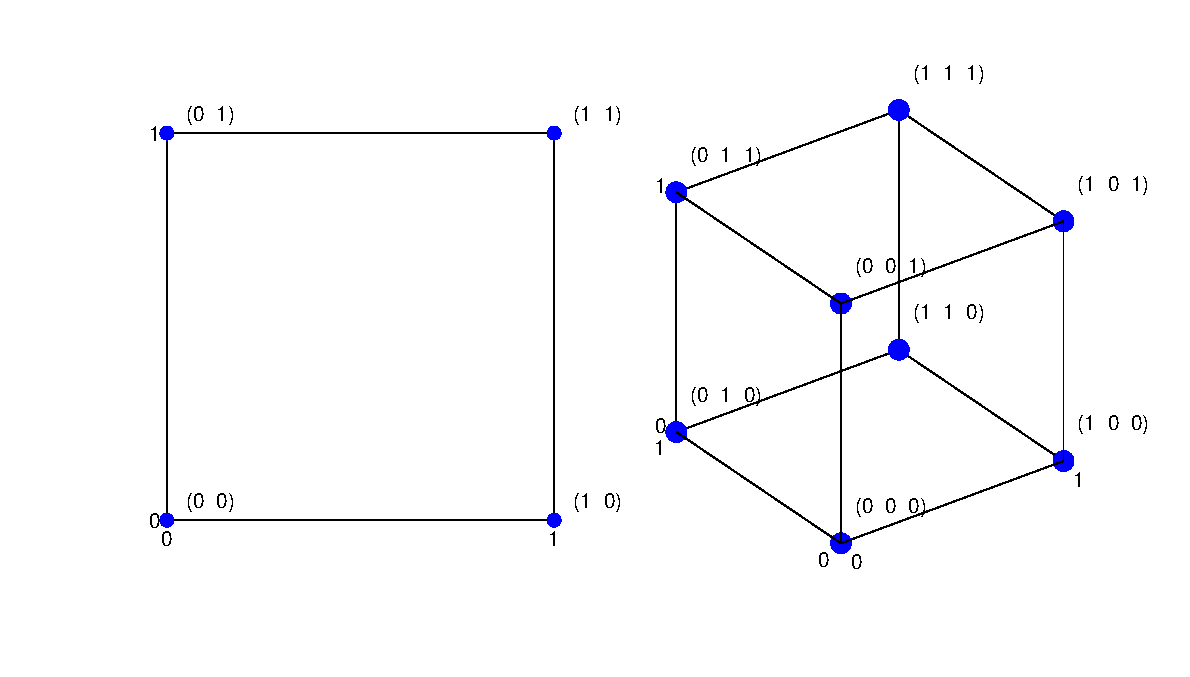
\includegraphics[width=4.5in]{figures/BernoulliDataSpace2and3}}
\end{figure}

\begin{definition}[Statistic]\label{D:Statistic}
A {\bf statistic} $T$ is any
%(measurable)
function of the data:
\[
T(x) : \Xz \to \Tz \ .
\]
Thus, a statistic $T$ is also an RV that takes values in the space $\Tz$.  When $x \in \Xz$ is the realisation of an experiment, we let $T(x)=t$ denote the corresponding realisation of the statistic $T$. Sometimes we use $T_n(X)$ and $\Tz_n$ to emphasise that $X$ is an $n$-dimensional random vector, i.e.~$\Xz \subset \Rz^n$
\end{definition}

\begin{classwork}[Is data a statistic?]
Is the RV $X$, for which the realisation is the observed data $X(\omega)=x$, a statistic?  In other words, is the data a statistic? [Hint: consider the identity map $T(x)=x: \Xz \to \Tz=\Xz$.]
\end{classwork}

Next, we define two important statistics called the {\bf sample mean} and {\bf sample variance}.  Since they are obtained from the sample data, they are called {\bf sample moments}, as opposed to the {\bf population moments}.  The corresponding population moments are $\E(X_1)$ and $\V(X_1)$, respectively.
\begin{definition}[Sample Mean]\label{D:SampleMean}
From a given a sequence of RVs $X_1,X_2,\ldots,X_n$, we may obtain another RV called the $n$-samples mean or simply the sample mean:
\begin{equation}\label{E:SampleMeanRV}
T_n( \ (X_1,X_2,\ldots,X_n) \ ) = \overline{X}_n( \ (X_1,X_2,\ldots,X_n) \ ) := \frac{1}{n} \sum_{i=1}^n X_i  \ .
\end{equation}
For brevity, we write $$\overline{X}_n( \ (X_1,X_2,\ldots,X_n) \ ) \quad \text{as} \quad \overline{X}_n \ ,$$ and its realisation $$\overline{X}_n( \ (x_1,x_2,\ldots,x_n) \ ) \quad \text{as} \quad \overline{x}_n \ .$$
\end{definition}
Note that the expectation and variance of $\overline{X}_n$ are:
\begin{eqnarray}
\E(\overline{X}_n) &=& \E \left(  \frac{1}{n} \sum_{i=1}^n X_i \right) \qquad \text{{\scriptsize[by \hyperref[E:SampleMeanRV]{definition \eqref{E:SampleMeanRV}}]}} \notag \\
&=&  \frac{1}{n} \sum_{i=1}^n \E \left( X_i \right) \qquad \text{{\scriptsize [by \hyperref[E:EofLinCombofRVs]{property \eqref{E:EofLinCombofRVs}}]}} \notag
\end{eqnarray}
Furthermore, if every $X_i$ in the original sequence of RVs $X_1,X_2,\ldots$ is {\bf identically} distributed with the same expectation, by convention $\E(X_1)$, then:
\begin{equation}\label{E:ExpOfSampleMeanOfIDSeq}
\E(\overline{X}_n)
= \frac{1}{n} \sum_{i=1}^n \E \left( X_i \right)
=  \frac{1}{n} \sum_{i=1}^n \E \left( X_1 \right)
=  \frac{1}{n} \ n \ \E \left( X_1 \right)  = \E \left( X_1 \right) \ .
\end{equation}
Similarly, we can show that:
\begin{eqnarray}
\V(\overline{X}_n) &=& \V \left(  \frac{1}{n} \sum_{i=1}^n X_i \right) \qquad \text{{\scriptsize[by \hyperref[E:SampleMeanRV]{definition \eqref{E:SampleMeanRV}}]}} \notag \\
&=& \left( \frac{1}{n} \right)^2  \V \left( \sum_{i=1}^n X_i \right) \qquad \text{{\scriptsize [by \hyperref[E:VofAffineofRVs]{property \eqref{E:VofAffineofRVs}}]}} \notag
\end{eqnarray}
Furthermore, if the original sequence of RVs $X_1,X_2,\ldots$ is {\bf independently} distributed then:
\begin{eqnarray}
\V(\overline{X}_n)
= \left( \frac{1}{n} \right)^2 \V \left(  \sum_{i=1}^n X_i \right)
=  \frac{1}{n^2} \ \sum_{i=1}^n \V \left( X_i \right) \qquad \text{{\scriptsize [by \hyperref[E:VofLinCombofRVs]{property \eqref{E:VofLinCombofRVs}}]}} \notag
\end{eqnarray}
Finally, if the original sequence of RVs $X_1,X_2,\ldots$ is {\bf independently and identically} distributed with the same variance ($\V(X_1)$ by convention) then:
\begin{equation}\label{E:VarOfSampleMeanOfIIDSeq}
\V(\overline{X}_n)
=  \frac{1}{n^2} \ \sum_{i=1}^n \V \left( X_i \right)
= \frac{1}{n^2} \ \sum_{i=1}^n \V \left( X_1 \right)
=  \frac{1}{n^2} \ n \ \V \left( X_1 \right)
=  \frac{1}{n} \ \V \left( X_1 \right) \ .
\end{equation}

\begin{labwork}[Sample mean]\label{LW:XsFromUni01Twstr101mean}
After initializing the fundamental sampler, we draw five samples and then obtain the sample mean using the {\sc Matlab} function {\tt mean}.  In the following, we will reuse the samples stored in the array {\tt XsFromUni01Twstr101}.
\begin{VrbM}
>> rand('twister',101); % initialise the fundamental Uniform(0,1) sampler
>> XsFromUni01Twstr101=rand(1,5); % simulate n=5 IID samples from Uniform(0,1) RV
>> SampleMean=mean(XsFromUni01Twstr101);% find sample mean
>> disp(XsFromUni01Twstr101); % The data-points x_1,x_2,x_3,x_4,x_5 are:
    0.5164    0.5707    0.0285    0.1715    0.6853
>> disp(SampleMean); % The Sample mean is :
    0.3945
\end{VrbM}
We can thus use {\tt mean} to obtain the sample mean $\overline{x}_n$ of $n$ sample points $x_1,x_2,\ldots,x_n$.

We may also obtain the sample mean using the {\tt sum} function and a division by sample size:
\begin{VrbM}
>> sum(XsFromUni01Twstr101) % take the sum of the elements of the XsFromUni01Twstr101 array
ans =    1.9723
>> sum(XsFromUni01Twstr101) / 5 % divide the sum by the sample size 5
ans =    0.3945
\end{VrbM}

We can also obtain the sample mean via matrix product or multiplication as follows:
\begin{VrbM}
>> size(XsFromUni01Twstr101) % size(SomeArray) gives the size or dimensions of the arrar SomeArray
ans =     1     5
>> ones(5,1) % here ones(5,1) is an array of 1's with size or dimension 5 X 1
ans =
     1
     1
     1
     1
     1
>> XsFromUni01Twstr101 * ones(5,1) % multiplying an 1 X 5 matrix with a 5 X 1 matrix of Ones
ans =    1.9723
>> XsFromUni01Twstr101 * ( ones(5,1) * 1/5) % multiplying an 1 X 5 matrix with a 5 X 1 matrix of 1/5 's
ans =    0.3945
\end{VrbM}
\end{labwork}

\begin{definition}[Sample Variance \& Standard Deviation]
From a given a sequence of random variables $X_1,X_2,\ldots,X_n$, we may obtain another statistic called the $n$-samples variance or simply the sample variance :
\begin{equation}\label{E:SampleVarianceRV}
T_n( \ (X_1,X_2,\ldots,X_n) \ ) = S^2_n( \ (X_1,X_2,\ldots,X_n) \ )  := \frac{1}{n-1} \sum_{i=1}^n {(X_i - \overline{X}_n)^2}  \ .
\end{equation}
For brevity, we write $S^2_n( \ (X_1,X_2,\ldots,X_n) \ )$ as $S^2_n$ and its  realisation $S^2_n( \ (x_1,x_2,\ldots,x_n) \ )$ as $s^2_n$.

Sample standard deviation is simply the square root of sample variance:
\begin{equation}\label{E:SampleStdDevRV}
S_n( \ (X_1,X_2,\ldots,X_n) \ ) = \sqrt{S^2_n( \ (X_1,X_2,\ldots,X_n) \ )}
\end{equation}
For brevity, we write $S_n( \ (X_1,X_2,\ldots,X_n) \ )$ as $S_n$ and its  realisation $S_n( \ (x_1,x_2,\ldots,x_n) \ )$ as $s_n$.
\end{definition}
Once again, if $X_1,X_2,\ldots,X_n \overset{\IID}{\sim} X_1$, the expectation of the sample variance is:
\[
\E(S^2_n) = \V(X_1) \ .
\]
\begin{labwork}[Sample variance and sample standard deviation]\label{LW:XsFromUni01Twstr101varstd}
We can compute the sample variance and sample standard deviation for the five samples stored in the array {\tt XsFromUni01Twstr101} from \hyperref[LW:XsFromUni01Twstr101mean]{Labwork \ref*{LW:XsFromUni01Twstr101mean}} using {\sc Matlab}'s functions {\tt var} and {\tt std}, respectively.
\begin{VrbM}
>> disp(XsFromUni01Twstr101); % The data-points x_1,x_2,x_3,x_4,x_5 are :
    0.5164    0.5707    0.0285    0.1715    0.6853
>> SampleVar=var(XsFromUni01Twstr101);% find sample variance
>> SampleStd=std(XsFromUni01Twstr101);% find sample standard deviation
>> disp(SampleVar) % The sample variance is:
    0.0785
>> disp(SampleStd) % The sample standard deviation is:
    0.2802
\end{VrbM}
\end{labwork}
It is important to bear in mind that the statistics such as sample mean and sample variance are random variables and have an underlying distribution.

\begin{definition}[Order Statistics]
Suppose $X_1,X_2,\ldots,X_n \overset{\IID}{\sim} F$, where $F$ is the DF from the set of all DFs over the real line.  Then, the $n$-sample {\bf order statistics} $X_{([n])}$ is:
\begin{equation}\label{E:OrderStatistics}
X_{([n])}( \ (X_1,X_2,\ldots,X_n) \ ) := \left(  X_{(1)},X_{(2)}, \ldots X_{(n)} \right), \text{ such that, }
 X_{(1)} \leq X_{(2)} \leq \ldots \leq X_{(n)}  \ .
\end{equation}
For brevity, we write $X_{([n])}( \ (X_1,X_2,\ldots,X_n) \ )$ as $X_{([n])}$ and its realisation $X_{([n])}( \ (x_1,x_2,\ldots,x_n) \ )$ as $x_{([n])} = (  x_{(1)},x_{(2)}, \ldots x_{(n)} )$.
\end{definition}
Without going into the details of how to sort the data in ascending order to obtain the order statistics (an elementary topic of an Introductory Computer Science course), we simply use {\sc Matlab}'s function {\tt sort} to obtain the order statistics, as illustrated in the following example.
\begin{labwork}[Order statistics and sorting]\label{LW:SortedXsFromUni01Twstr101}
The order statistics for the five samples stored in {\tt XsFromUni01Twstr101} from \hyperref[LW:XsFromUni01Twstr101mean]{Labwork \ref*{LW:XsFromUni01Twstr101mean}} can be computed using {\tt sort} as follows:
\begin{VrbM}
>> disp(XsFromUni01Twstr101); % display the sample points
    0.5164    0.5707    0.0285    0.1715    0.6853
>> SortedXsFromUni01Twstr101=sort(XsFromUni01Twstr101); % sort data
>> disp(SortedXsFromUni01Twstr101); % display the order statistics
    0.0285    0.1715    0.5164    0.5707    0.6853
\end{VrbM}
Therefore, we can use {\tt sort} to obtain our order statistics $x_{(1)},x_{(2)},\ldots,x_{(n)}$ from $n$ sample points $x_1,x_2,\ldots,x_n$.
\end{labwork}

Next, we will introduce a family of common statistics, called the $q^{\text{th}}$ quantile, by first defining the function:
\begin{definition}[Inverse DF or Inverse CDF or Quantile Function]
Let $X$ be an RV with DF $F$.  The {\bf inverse DF} or {\bf inverse CDF} or {\bf quantile function} is:
\begin{equation}\label{E:InverseCDF}
F^{[-1]}(q) := \inf { \{ x: F(x) > q \}}, \quad \text{ for some $q \in [0,1]$} \ .
\end{equation}
If $F$ is strictly increasing and continuous then $F^{[-1]}(q)$ is the unique $x \in \Rz$ such that $F(x)=q$.
\end{definition}
A {\bf functional} is merely a function of another function.  Thus, $T(F): \{ \text{All DFs }\} \to \Tz$, being a map or function from the space of DFs to its range $\Tz$, is a functional.  Some specific examples of functionals we have already seen include:
\begin{enumerate}
\item The {\bf mean} of RV $X \sim F$ is a function of the DF $F$:
\[
T(F) = \E(X) = \int x\,dF(x) \ .
\]
\item The {\bf variance} of RV $X \sim F$ is a function of the DF $F$:
\[
T(F) = \E(X-\E(X))^2 = \int (x-\E(X))^2\,dF(x) \ .
\]
\item The {\bf value of DF at a given $x \in \Rz$} of RV $X \sim F$ is also a function of DF $F$:
\[
T(F) = F(x) \  .
\]
\end{enumerate}
Other functionals of $F$ that depend on the quantile function $F^{[-1]}$ are:
\begin{enumerate}
\item The {\bf $q^{\text{th}}$ quantile} of RV $X \sim F$:
\[
T(F) = F^{[-1]}(q) \ \text{ where } q \in [0,1] \ .
\]
\item The {\bf first quartile} or the {\bf $0.25^{\text{th}}$ quantile} of the RV $X \sim F$:
\[
T(F) = F^{[-1]}(0.25) \ .
\]
\item The {\bf median} or the {\bf second quartile} or the {\bf $0.50^{\text{th}}$ quantile} of the RV $X \sim F$:
\[
T(F) = F^{[-1]}(0.50) \  .
\]
\item The {\bf third quartile} or the {\bf $0.75^{\text{th}}$ quantile} of the RV $X \sim F$:
\[
T(F) = F^{[-1]}(0.75) \ .
\]
\end{enumerate}

\begin{definition}[Empirical Distribution Function (EDF or ECDF)]\label{D:ECDF}
Suppose we have $n$ IID RVs, $X_1,X_2,\ldots,X_n \overset{\IID}{\sim} F$, where $F$ is a DF from the set of all DFs over the real line.  Then, the $n$-sample empirical distribution function (EDF or ECDF) is the discrete  distribution function $\widehat{F}_n$ that puts a probability mass of $1/n$ at each sample or data point $x_i$:
\begin{eqnarray} \label{E:ECDF}
\widehat{F}_n(x) = \frac{ \sum_{i=1}^n \BB{1}(X_i \leq x) }{n} \ ,  & \quad where \qquad
\BB{1}(X_i \leq x) :=
\begin{cases}
& 1  \quad \text{if $x_i \leq x$} \\
& 0  \quad \text{if $x_i > x$}
\end{cases}
\end{eqnarray}
\end{definition}

\begin{labwork}[Plot of empirical CDF]\label{LW:ECDF}
Let us plot the ECDF for the five samples drawn from the $Uniform(0,1)$ RV in \hyperref[LW:XsFromUni01Twstr101mean]{Labwork \ref*{LW:XsFromUni01Twstr101mean}} using the {\sc Matlab} function {\tt ECDF}. %(given in \hyperref[Mf:ECDF]{Labwork \ref*{Mf:ECDF}}).
Let us super-impose the samples and the true DF as depicted in \hyperref[F:plotUniform01ECDF5]{Figure \ref*{F:plotUniform01ECDF5}} with the following script:
{\VrbMf[label=plotunifecdf.m]{scripts/plotunifecdf.m}}

\begin{figure}[htpb]
\caption{Plot of the DF of $\uniform(0,1)$, five IID samples from it, and the ECDF $\widehat{F}_5$ for these five data points $x=(x_1,x_2,x_3,x_4,x_5)=(0.5164,    0.5707,    0.0285,    0.1715,    0.6853)$ that jumps by $1/5=0.20$ at each of the five samples.\label{F:plotUniform01ECDF5}}
\centering   \makebox{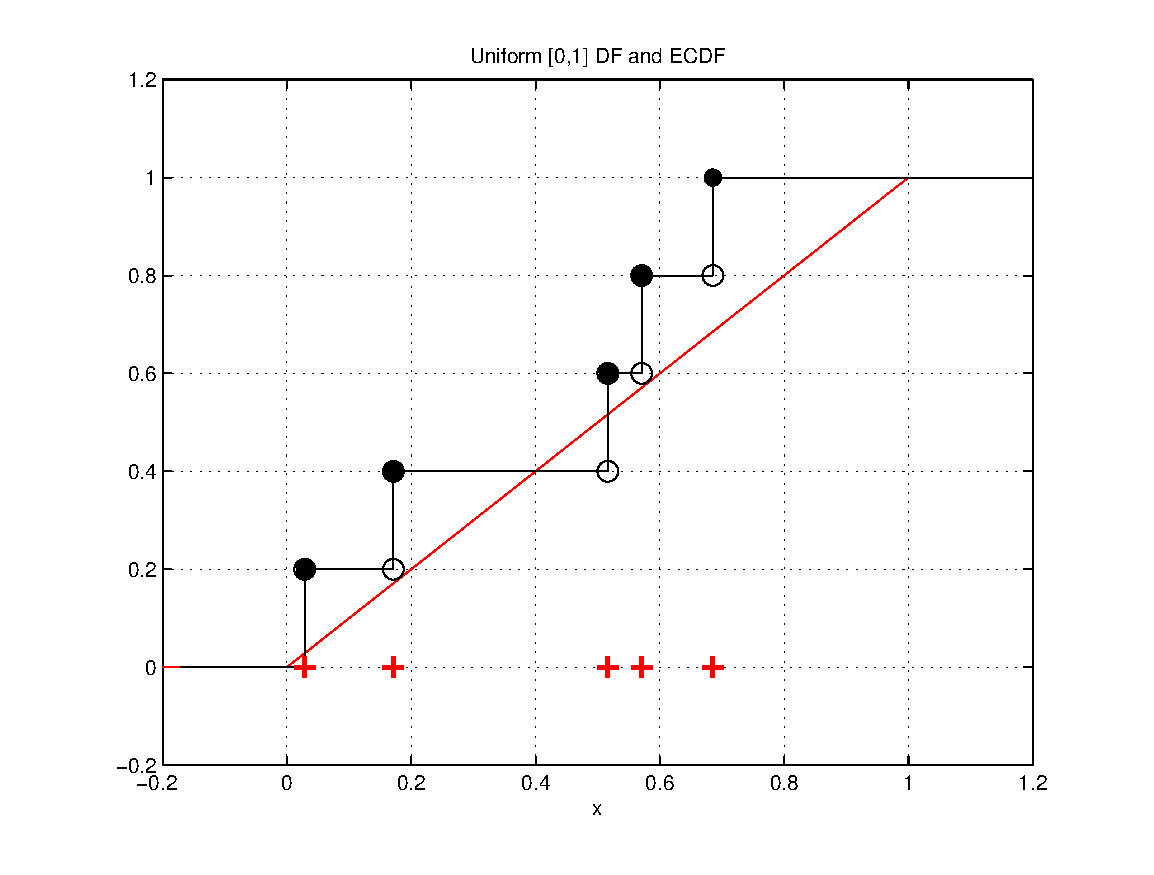
\includegraphics[width=4.5in]{figures/plotUniform01ECDF5}}
\end{figure}
\end{labwork}

\begin{definition}[$q^{\text{th}}$ Sample Quantile]
For some $q \in [0,1]$ and $n$ IID RVs $X_1,X_2,\ldots,X_n \overset{\IID}{\sim} F$, we can obtain the ECDF $\widehat{F}_n$ using \eqref{E:ECDF}.  The {\bf $q^{\text{th}}$ sample quantile} is defined as the statistic (statistical functional):
\begin{equation}\label{E:qthSampleQuantile}
T(\widehat{F}_n) = \widehat{F}_n^{[-1]}(q) := \inf{ \{ x:  \widehat{F}_n^{[-1]}(x) \geq q \} } \ .
\end{equation}
By replacing $q$ in this definition of the $q^{\text{th}}$ sample quantile by $0.25$, $0.5$ or $0.75$, we obtain the first, second ({\bf sample median}) or third {\bf sample quartile}, respectively.
\end{definition}

The following algorithm can be used to obtain the $q^{\text{th}}$ sample quantile of $n$ IID samples $(x_1,x_2,\ldots,x_n)$ on the basis of their order statistics $(x_{(1)},x_{(2)},\ldots,x_{(n)})$.
\begin{algorithm}
\caption{$q^{\text{th}}$ Sample Quantile of Order Statistics}
\label{A:qthSampleQuantile}
\begin{algorithmic}[1]
\STATE {
{\it input:}
\begin{enumerate}
\item $q$ in the $q^{\text{th}}$ sample quantile, i.e.~the argument $q$ of $ \widehat{F}_n^{[-1]}(q)$,
\item order statistic $(x_{(1)},x_{(2)},\ldots,x_{(n)})$, i.e.~the sorted $(x_1,x_2,\ldots,x_n)$, where $n>0$.
\end{enumerate}
}
\STATE {\it output:} $ \widehat{F}_n^{[-1]}(q)$, the $q^{\text{th}}$ sample quantile
\STATE $i \gets \lfloor (n-1) q \rfloor$
\STATE $\delta \gets (n-1) q - i$
\IF {$i = n-1$}
\STATE {$ \widehat{F}_n^{[-1]}(q) \gets x_{(i+1)}$}
\ELSE
\STATE $ \widehat{F}_n^{[-1]}(q) \gets (1 - \delta) x_{(i+1)} + \delta x_{(i+2)}$
\ENDIF
\STATE {{\it return:} $ \widehat{F}_n^{[-1]}(q)$}
\end{algorithmic}
\end{algorithm}

The $q^{\text{th}}$ sample quantile, $ \widehat{F}_n^{[-1]}(q)$, is found by interpolation from the order statistics $(x_{(1)},x_{(2)},\ldots,x_{(n)})$ of the $n$ data points $(x_1,x_2,\ldots,x_n)$, using the formula:
\[
 \widehat{F}_n^{[-1]}(q) = (1 - \delta) x_{(i+1)} + \delta x_{(i+2)}, \quad \text{where, }
\quad i = \lfloor (n-1) q \rfloor  \quad \text{ and }
\quad \delta = (n-1) q -  \lfloor (n-1) q \rfloor \ .
\]
Thus, the {\bf sample minimum} of the data points $(x_1,x_2,\ldots,x_n)$ is given by $ \widehat{F}_n^{[-1]}(0)$, the {\bf sample maximum} is given by $ \widehat{F}_n^{[-1]}(1)$ and the {\bf sample median} is given by $ \widehat{F}_n^{[-1]}(0.5)$, etc.
\begin{labwork}[The $q^{\text{th}}$ sample quantile]\label{LW:qthSampleQuantile}
Use the implementation of \hyperref[A:qthSampleQuantile]{Algorithm \ref*{A:qthSampleQuantile}} %in \hyperref[Mf:qthSampleQuantile]{Labwork \ref*{Mf:qthSampleQuantile}}
as the {\sc Matlab} function {\tt qthSampleQuantile} to find the $q^{\text{th}}$ sample quantile of two simulated data arrays:
\begin{enumerate}
\item {\tt SortedXsFromUni01Twstr101}, the order statistics that was constructed in \hyperref[LW:SortedXsFromUni01Twstr101]{Labwork \ref*{LW:SortedXsFromUni01Twstr101}} and
\item Another sorted array of $7$ samples called {\tt SortedXs}
\end{enumerate}
\begin{VrbM}
>> disp(SortedXsFromUni01Twstr101)
    0.0285    0.1715    0.5164    0.5707    0.6853
>> rand('twister',420);
>> SortedXs=sort(rand(1,7));
>> disp(SortedXs)
    0.1089    0.2670    0.3156    0.3525    0.4530    0.6297    0.8682
>> for q=[0, 0.25, 0.5, 0.75, 1.0]
       disp([q, qthSampleQuantile(q,SortedXsFromUni01Twstr101) ...
                qthSampleQuantile(q,SortedXs)])
   end
         0    0.0285    0.1089
    0.2500    0.1715    0.2913
    0.5000    0.5164    0.3525
    0.7500    0.5707    0.5414
    1.0000    0.6853    0.8682
\end{VrbM}
\end{labwork}

%\subsection{Exploring Data and Statistics}\label{S:ExploringData}

\subsection{Univariate Data}
A {\bf histogram} is a graphical representation of the frequency with which elements of a data array:
$$x = (x_1,x_2,\ldots,x_n) \ ,$$
of real numbers fall within each of the $m$ intervals or {\bf bins} of some {\bf interval partition}:
$$b := ( b_1, b_2, \ldots, b_m ) := ( [\underline{b}_1,\overline{b}_1], [\underline{b}_2,\overline{b}_2], \ldots, [\underline{b}_m,\overline{b}_m] )$$
of the {\bf data range} of $x$ given by the closed interval:
$$\C{R}(x) := [\min \{x_1,x_2,\ldots,x_n \}, \max \{x_1,x_2,\ldots,x_n \}] \ .$$
Elements of this partition $b$ are called bins, their mid-points are called {\bf bin centres}:
$$c := ( c_1, c_2, \ldots, c_m ) := ( (\underline{b}_1+\overline{b}_1)/2, (\underline{b}_2 + \overline{b}_2)/2, \ldots, (\underline{b}_m + \overline{b}_m)/2 )$$
and their overlapping boundaries, i.e.~$\overline{b}_i=\underline{b}_{i+1}$ for $1 \leq i < m$, are called {\bf bin edges}:
$$d := (d_1,d_2,\ldots,d_{m+1}) := (\underline{b}_1, \underline{b}_2, \ldots, \underline{b}_{m-1}, \underline{b}_m, \overline{b}_m) \ .$$
For a given partition of the data range $\C{R}(x)$ or some superset of $\C{R}(x)$, three types of histograms are possible: frequency histogram, relative frequency histogram and density histogram.  Typically, the partition $b$ is assumed to be composed of $m$ overlapping intervals of the same width $w=\overline{b}_i - \underline{b}_i$ for all $i=1,2,\ldots,m$.  Thus, a histogram can be obtained by a set of bins along with their corresponding {\bf heights}:
$$h = (h_1,h_2,\ldots,h_m) \ , \text{ where } h_k := g(\# \{x_i : x_i \in b_k\} )$$
Thus, $h_k$, the height of the $k$-th bin, is some function $g$ of the number of data points that fall in the bin $b_k$ Formally, a histogram is a sequence of ordered pairs:
$$\left(  (b_1,h_1), (b_2,h_2), \ldots, (b_m,h_m) \right) \ .$$

Given a partition $b$, a {\bf frequency histogram} is the histogram:
$$\left(  (b_1,h_1), (b_2,h_2), \ldots, (b_m,h_m) \right) \ , \text{ where } h_k := \# \{x_i : x_i \in b_k\} \ ,$$
a {\bf relative frequency histogram} is the histogram:
$$\left(  (b_1,h_1), (b_2,h_2), \ldots, (b_m,h_m) \right) \ , \text{ where } h_k := n^{-1} \# \{x_i : x_i \in b_k\} \ ,$$
and a {\bf density histogram} is the histogram:
$$\left(  (b_1,h_1), (b_2,h_2), \ldots, (b_m,h_m) \right) \ , \text{ where } h_k := (w_k n)^{-1} \# \{x_i : x_i \in b_k\} \ , w_k := \overline{b}_k - \underline{b}_k \ .$$

\begin{figure}[htpb]
\caption{Frequency, Relative Frequency and Density Histograms\label{F:FreqRelFreqDensityHistograms100Unif01MT5489}}
\centering   \makebox{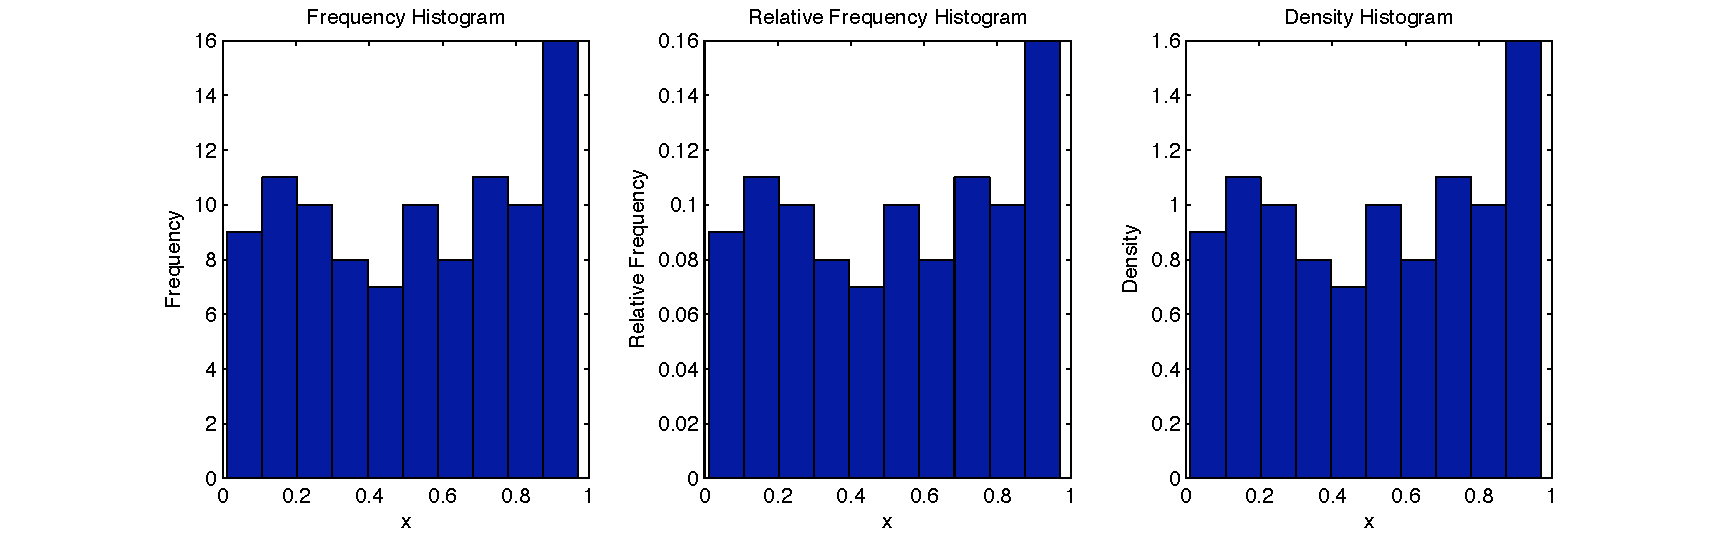
\includegraphics[width=6.5in]{figures/FreqRelFreqDensityHistograms100Unif01MT5489}}
\end{figure}

\begin{labwork}[Histograms with specified number of bins for univariate data]\label{LW:hist}
Let us use samples from the {\tt rand('twister',5489)} as our data set $x$ and plot various histograms.  Let us use {\tt hist} function (read {\tt help hist}) to make a default histogram with ten bins.  Then we can make three types of histogarms as shown in \hyperref[F:FreqRelFreqDensityHistograms100Unif01MT5489]{Figure~\ref*{F:FreqRelFreqDensityHistograms100Unif01MT5489}}  as follows:
\begin{VrbM}
>> rand('twister',5489);
>> x=rand(1,100); % generate 100 PRNs
>> hist(x) % see what default hist does in Figure Window
>> % Now let us look deeper into the last hist call
>> [Fs, Cs] = hist(x) % Cs is the bin centers and Fs is the frequencies of data set x
Fs =
     9    11    10     8     7    10     8    11    10    16
Cs =
    0.0598    0.1557    0.2516    0.3474    0.4433    0.5392    0.6351    0.7309    0.8268    0.9227
>> % produce a histogram plot the last argument 1 is the width value for immediately adjacent bars -- help bar
>> bar(Cs,Fs,1) % create a frequency histogram
>> bar(Cs,Fs/100,1) % create a relative frequency histogram
>> bar(Cs,Fs/(0.1*100),1) % create a density histogram (area of bars sum to 1)
>> sum(Fs/(0.1*100) .* ones(1,10)*0.1) % checking if area does sum to 1
>> ans = 1
\end{VrbM}
Try making a density histogram with 1000 samples from {\tt rand} with 15 bins.  You can specify the number of bins by adding an extra argument to {\tt hist}, for e.g. {\tt [Fs, Cs] = hist(x,15)} will produce 15 bins of equal width over the data range $\C{R}(x)$.
\end{labwork}

\begin{labwork}[Stem plots and ECDF plots for univariate data]\label{LW:StemEcdf}
We can also visualise the 100 data points in the array {\tt x} using stem plot and ECDF plot as shown in \hyperref[F:StemECDF100Unif01MT5489]{Figure~\ref*{F:StemECDF100Unif01MT5489}} as follows:
\begin{VrbM}
>> rand('twister',5489);
>> x=rand(1,100); % produce 100 samples with rand
>> stem(x,'.') % make a stem plot of the 100 data points in x (the option '.' gives solid circles for x)
>>% ECDF (type help ECDF) plot is extended to left and right by .2 and .6, respectively
>>% (second parameter 6 makes the dots in the plot smaller).
>> ECDF(x,6,.2,.6);
\end{VrbM}
\end{labwork}

\begin{figure}[htpb]
\caption{Frequency, Relative Frequency and Density Histograms\label{F:StemECDF100Unif01MT5489}}
\centering   \makebox{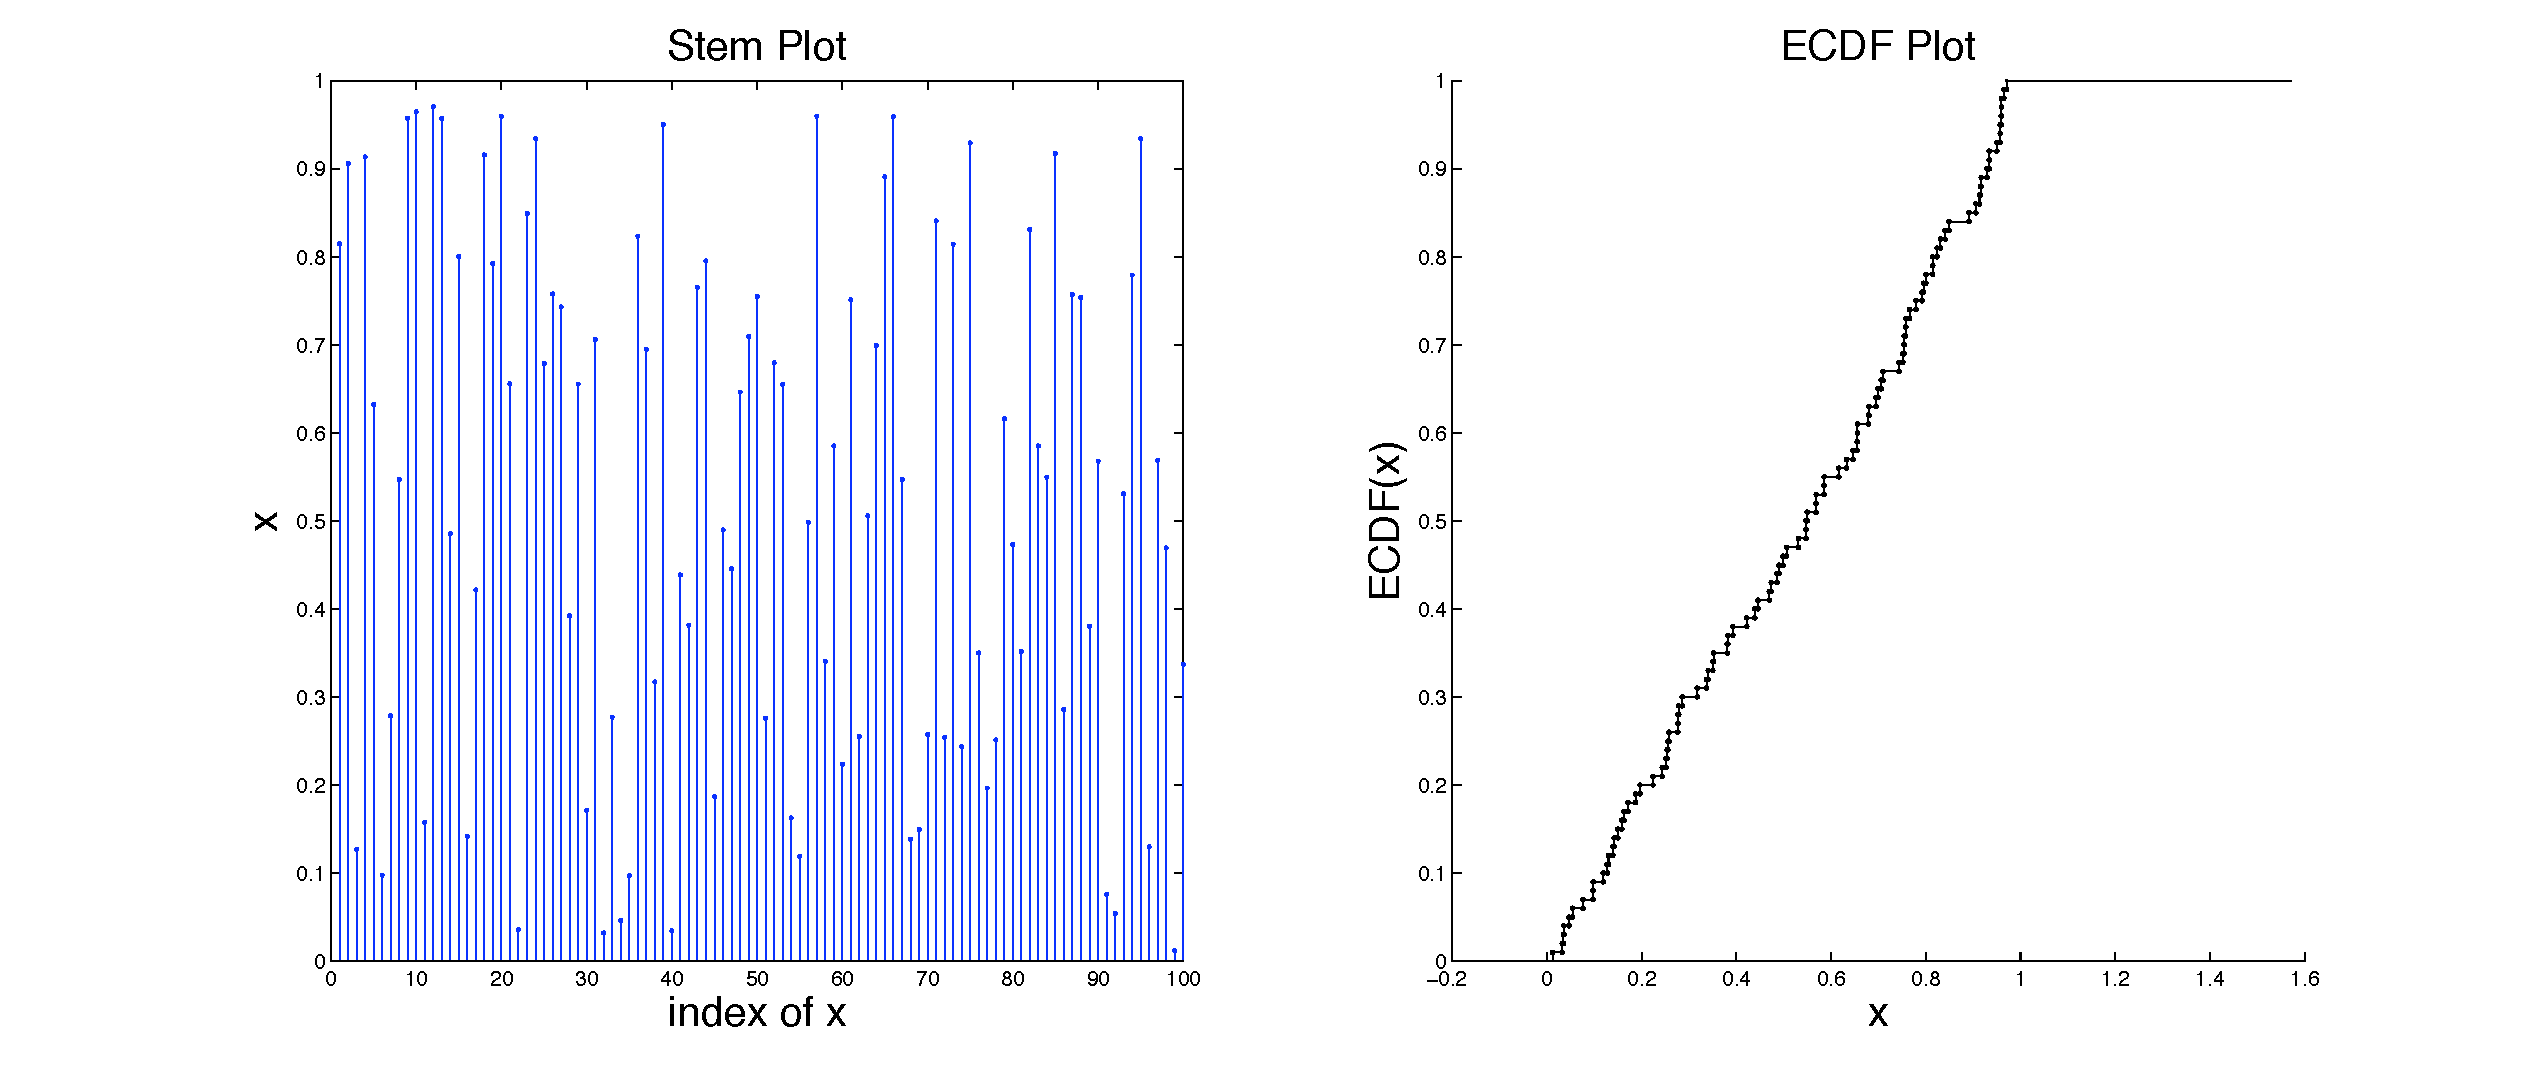
\includegraphics[width=6.5in]{figures/StemECDF100Unif01MT5489}}
\end{figure}

We can also visually summarise univariate data using the {\bf box plot} or {\bf box-whisker plot} available in the Stats Toolbox of {\sc Matlab}.  These family of plots display a set of sample quantiles, typically they are include, the median, the first and third quartiles and the minimum and maximum values of our data array $x$.

\subsection{Bivariate Data}
By bivariate data array $x$ we mean a $2 \times n$ matrix of real numbers or equivalently $n$ ordered pairs of points $(x_{1,i},x_{2,i})$ as $i=1,2,\ldots,n$.  The most elementary visualisation of these $n$ ordered pairs is in orthogonal Cartesian co-ordinates.  Such plots are termed 2D {\bf scatter plots} in statistics.
\begin{labwork}[Visualising bivariate data]\label{LW:2DScatter}
Let us generate a $2 \times 5$ array representing samples of $5$ ordered pairs sampled uniformly at random over the unit square $[0,1] \times [0,1]$.  We can make 2D scatter plot as shown in \hyperref[F:Twister5489X2x5Scatter2D]{Figure~\ref*{F:Twister5489X2x5Scatter2D}}  as follows:
\begin{VrbM}
>> rand('twister',5489);
>> x=rand(2,5)% create a sequence of 5 ordered pairs uniformly from unit square [0,1]X[0,1]
x =
    0.8147    0.1270    0.6324    0.2785    0.9575
    0.9058    0.9134    0.0975    0.5469    0.9649
>> plot(x(1,:),x(2,:),'x') % a 2D scatter plot with marker cross or 'x'
>> plot(x(1,:),x(2,:),'x', 'MarkerSize',15) % a 2D scatter plot with marker cross or 'x' and larger Marker size
>> xlabel('x_1'); ylabel('x_2'); % label the axes
\end{VrbM}
\end{labwork}

\begin{figure}[htpb]
\caption{2D Scatter Plot\label{F:Twister5489X2x5Scatter2D}}
\centering   \makebox{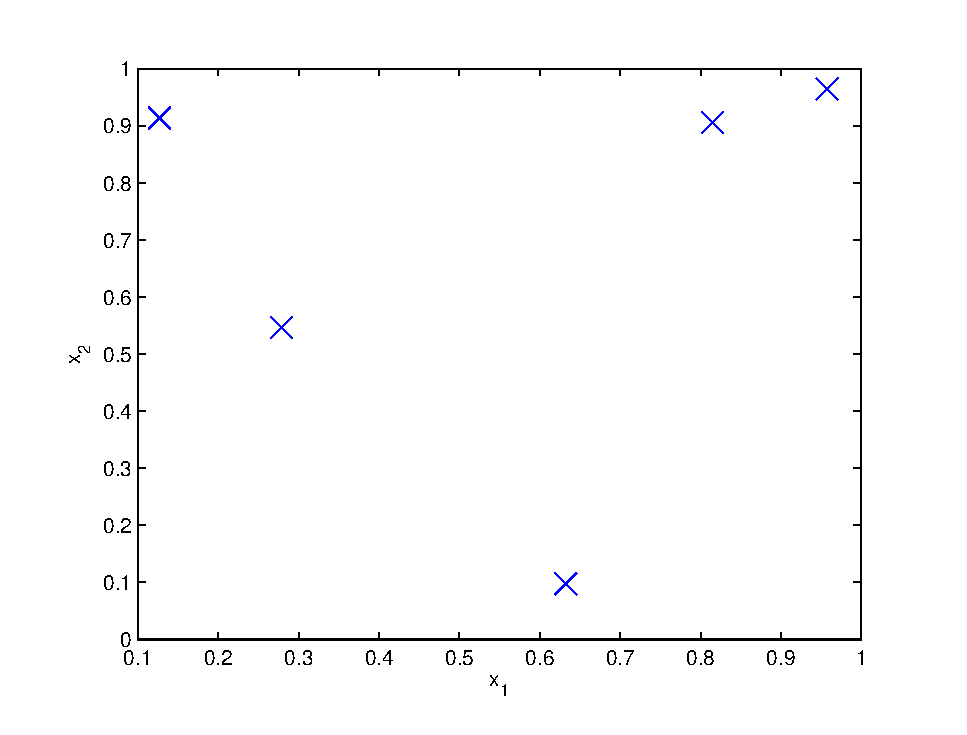
\includegraphics[width=4.5in]{figures/Twister5489X2x5Scatter2D}}
\end{figure}

There are several other techniques for visualising bivariate data, including,
2D histograms, surface plots, heat plots, and we will encounter some of them in the sequel.

\subsection{Trivariate Data}
Trivariate data is more difficult to visualise on paper but playing around with the rotate 3D feature in \Matlab's Figure window can help bring a lot more perspective.

\begin{labwork}[Visualising trivariate data]\label{LW:3DScatter}
We can make {\bf 3D scatter plots} as shown in \hyperref[F:Twister5489X3x5Scatter3D]{Figure~\ref*{F:Twister5489X3x5Scatter3D}}  as follows:
\begin{VrbM}
>> rand('twister',5489);
>> x=rand(3,5)% create a sequence of 5 ordered triples uniformly from unit cube [0,1]X[0,1]X[0,1]
x =
    0.8147    0.9134    0.2785    0.9649    0.9572
    0.9058    0.6324    0.5469    0.1576    0.4854
    0.1270    0.0975    0.9575    0.9706    0.8003
>> plot3(x(1,:),x(2,:),x(3,:),'x') % a simple 3D scatter plot with marker 'x'
>>% a more interesting one with options that control marker type, line-style,
>>% colour in [Red Green Blue] values and marker size - read help plot3 for more options
>> plot3(x(1,:),x(2,:),x(3,:),'Marker','*','LineStyle','none','Color',[1 0 1],'MarkerSize',15)
>> plot3(x(1,:),x(2,:),x(3,:),'m*','MarkerSize',15) % makes same  figure as before but shorter to write
>> box on % turn on the box and see the effect on the Figure
>> grid on % turn on the grid and see the effect on the Figure
>> xlabel('x_1'); ylabel('x_2'); zlabel('x_3'); % assign labels to x,y and z axes
\end{VrbM}
Repeat the visualisation below with a larger array, say {\tt x=rand(3,1000)}, and use the rotate 3D feature in the Figure window to visually explore the samples in the unit cube.  Do they seem to be uniformly distributed inside the unit cube?
\end{labwork}

\begin{figure}[htpb]
\caption{3D Scatter Plot\label{F:Twister5489X3x5Scatter3D}}
\centering   \makebox{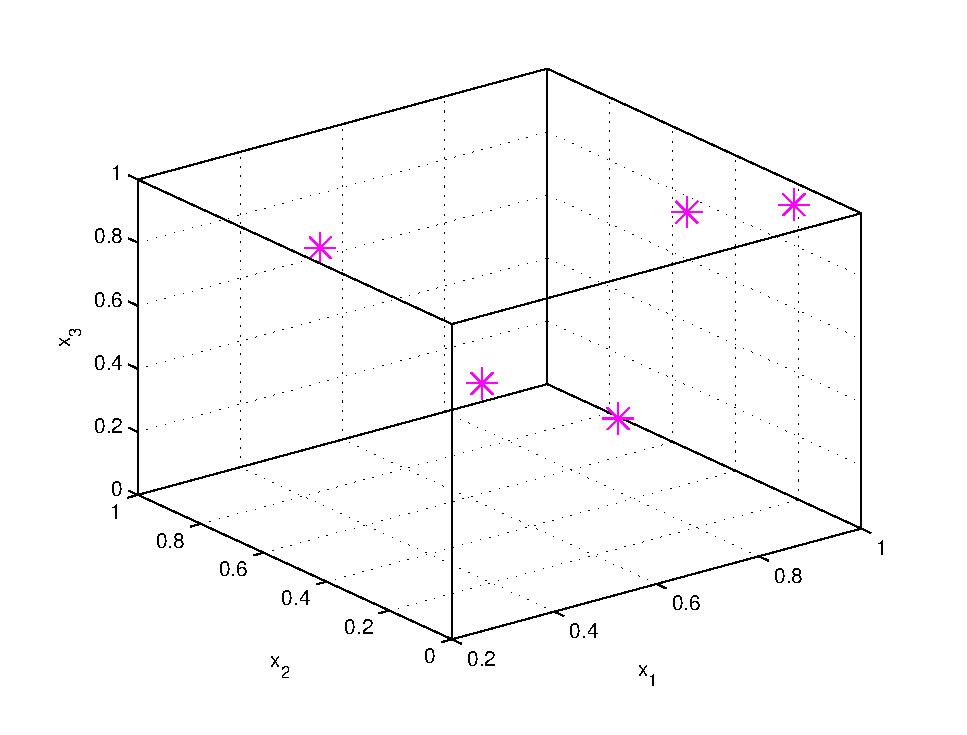
\includegraphics[width=4.5in]{figures/Twister5489X3x5Scatter3D}}
\end{figure}


There are several other techniques for visualising trivariate data, including,
iso-surface plots, moving surface or heat plots, and you will encounter some of them in the future.

\subsection{Multivariate Data}
For high-dimensional data in $d$-dimensional space $\Rz^d$ with $d \geq 3$ you have to look at several lower dimensional projections of the data.  We can simultaneously look at 2D scatter plots for every pair of co-ordinates $\{(i,j) \in \{1,2,\ldots,d\}^2 : i \neq j \}$ and at histograms for every co-ordinate $i \in \{1,2,\ldots,d\}$ of the $n$ data points in $\Rz^d$.  Such a set of low-dimensional projections can be conveniently represented in a $d \times d$ matrix of plots called a {\bf matrix plot}.

\begin{figure}[htpb]
\caption{Plot Matrix of uniformly generated data in $[0,1]^5$\label{F:Twister5489X100x5PlotMatrixFirst6andAll100}}
\centering
\mbox{\subfigure[First six samples]{\hspace{-1.cm} 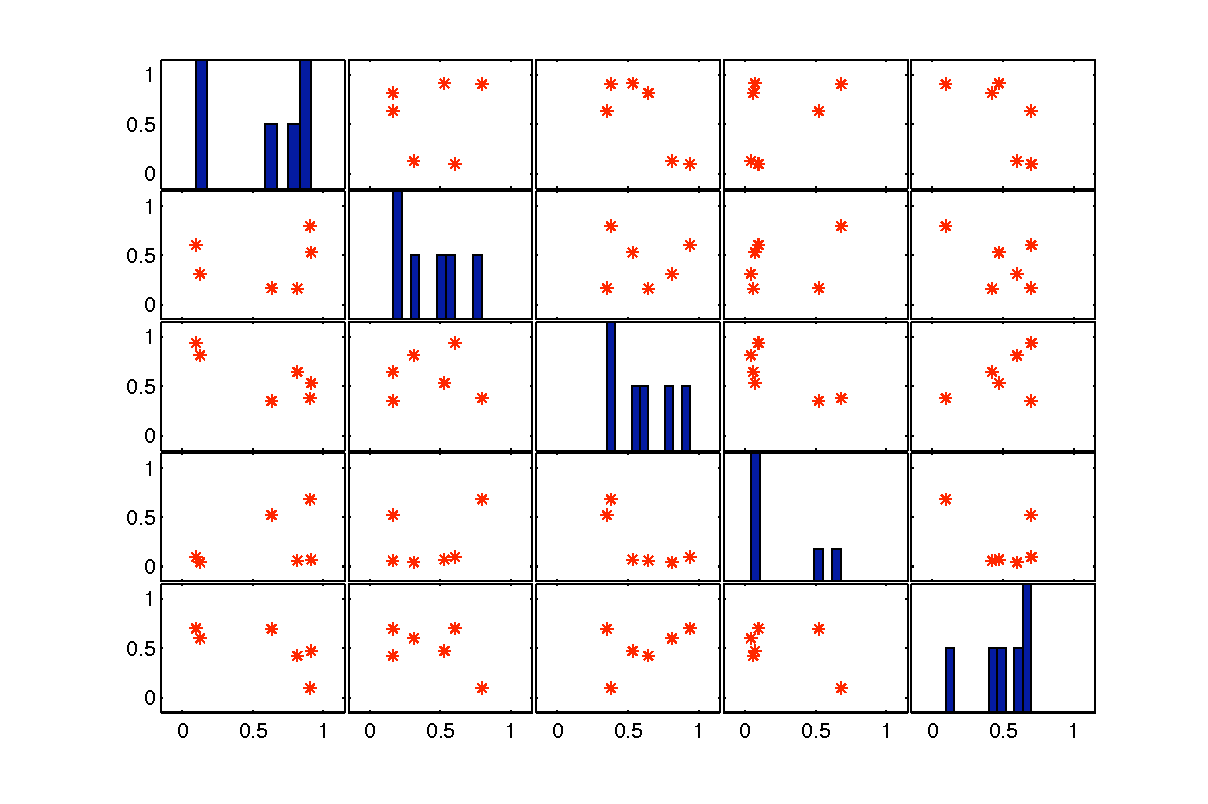
\includegraphics[width=3.750in]{figures/Twister5489X100x5PlotMatrixFirst6}} \hspace{-1.cm}
	   \subfigure[All thousand samples]{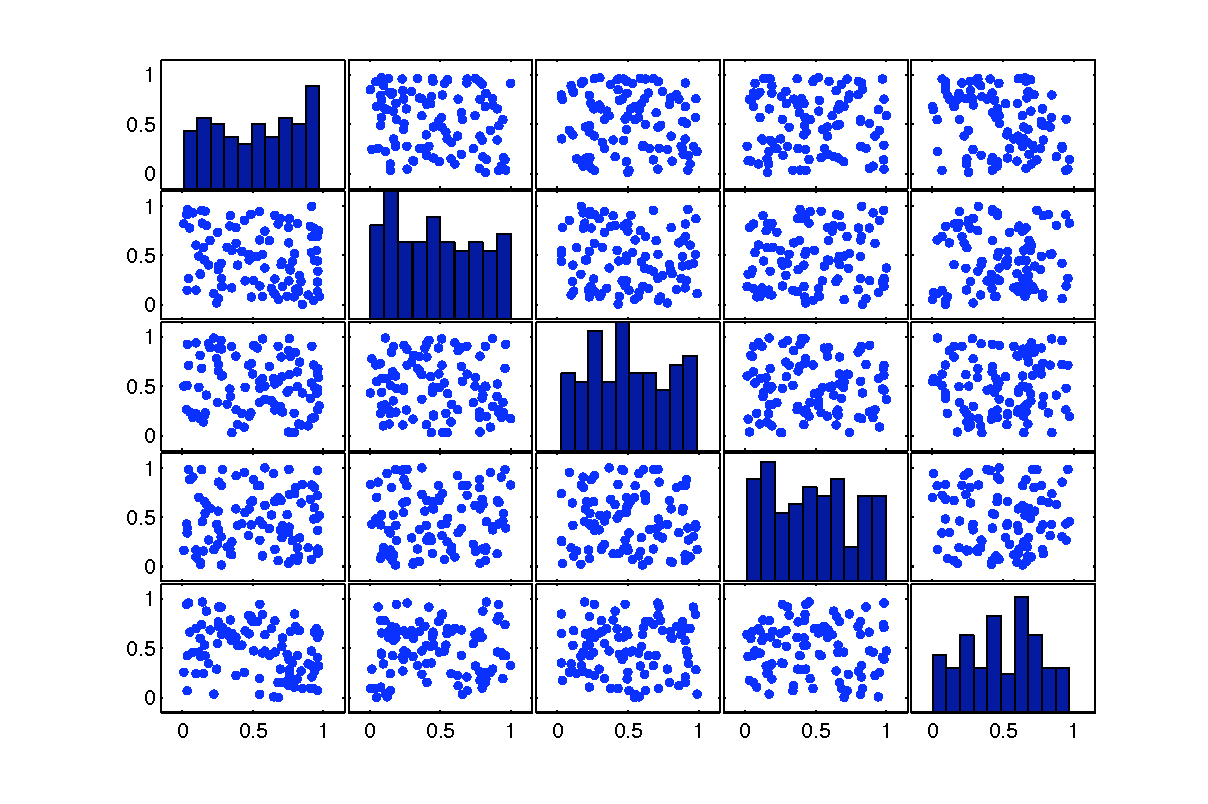
\includegraphics[width=3.750in]{figures/Twister5489X100x5PlotMatrixAll100}} }
\end{figure}

\begin{labwork}\label{LW:matrixplot5DUniform}
Let us make matrix plots from a uniformly generated  sequence of $100$ points in 5D unit cube $[0,1]^5$ as shown in \hyperref[F:Twister5489X100x5PlotMatrixFirst6andAll100]{Figure~\ref*{F:Twister5489X100x5PlotMatrixFirst6andAll100}}.
\begin{VrbM}
>> rand('twister',5489);
>> % generate a sequence of 1000 points uniformly distributed in 5D unit cube [0,1]X[0,1]X[0,1]X[0,1]X[0,1]
>> x=rand(1000,5);
>> x(1:6,:) % first six points in our 5D unit cube, i.e., the first six rows of x
ans =
    0.8147    0.6312    0.7449    0.3796    0.4271
    0.9058    0.3551    0.8923    0.3191    0.9554
    0.1270    0.9970    0.2426    0.9861    0.7242
    0.9134    0.2242    0.1296    0.7182    0.5809
    0.6324    0.6525    0.2251    0.4132    0.5403
    0.0975    0.6050    0.3500    0.0986    0.7054
>> plotmatrix(x(1:5,:),'r*') % make a plot matrix
>> plotmatrix(x) % make a plot matrix of all 1000 points
\end{VrbM}
\end{labwork}


\subsection{Loading and Exploring Real-world Data}\label{S:EDA}

All of the data we have played with so far were computer-generated.  It is time to get our hands dirty with real-world data.  The first step is to obtain the data.
Often, publicly-funded institutions allow the public to access their databases.  Such data can be fetched from appropriate URLs in one of the two following ways:
\begin{itemize}
\item[{\sf Method~A}:] Manually download by filling the appropriate fields in an online request form.
\item[{\sf Method~B}:] Automagically download directly from your \Matlab session.
\end{itemize}
Then we want to inspect it for inconsistencies, missing values and replace them with {\tt NaN} values in \Matlab that stand for not-any-number.  Finally, we can visually explore, transform and interact with the data to discover interesting patterns that are hidden in the data.  This process is called {\em exploratory data analysis} and is the foundational first step towards subsequent computational statistical experiments [{\em John W.~Tukey, Exploratory Data Analysis, Addison-Wesely, New York, 1977}].

\subsection{Geological Data}
 Let us focus on the data of earth quakes that heavily damaged Christchurch on February 22 2011.  This data can be fetched from the URL \href{http://magma.geonet.org.nz/resources/quakesearch/}{\url{http://magma.geonet.org.nz/resources/quakesearch/}} by {\sf Method A} and loaded into \Matlab for exploratory data analysis as done in \hyperref[LW:NZEQChCch20110222]{Labwork~\ref*{LW:NZEQChCch20110222}}.

 \begin{labwork}\label{LW:NZEQChCch20110222}
Let us go through the process one step at a time using {\sf Method~A}.
\begin{enumerate}
\item Download the data as a CSV or {\em comma separated variable} file in plain ASCII text (this has been done for this data already for you and saved as {\tt NZ20110222earthquakes.csv} in the {\tt CSEMatlabScripts} directory).
\item Open the file in a simple text editor such as {\tt Note Pad} in Windows or one of the following editors in OS X, Unix, Solaris, Linux/GNU variants such as Ubuntu, SUSE, etc: {\tt vi}, {\tt vim}, {\tt emacs}, {\tt geany}, etc.  The first three and last two lines of this file look as follows:
\begin{VrbM}
CUSP_ID,LAT,LONG,NZMGE,NZMGN,ORI_YEAR,ORI_MONTH,ORI_DAY,ORI_HOUR,ORI_MINUTE,ORI_SECOND,MAG,DEPTH
3481751,-43.55432,172.68898,2484890,5739375,2011,2,22,0,0,31.27814,3.79,5.8559,
3481760,-43.56579,172.70621,2486287,5738106,2011,2,22,0,0,43.70276,3.76,5.4045,
.
.
.
3469114,-43.58007,172.67126,2483470,5736509,2011,2,22,23,28,11.1014,3.117,3,
3469122,-43.55949,172.70396,2486103,5738805,2011,2,22,23,50,1.06171,3.136,12,
\end{VrbM}
The thirteen columns correspond to fairly self-descriptive features of each measured earth quake given in the first line or row.  They will become clear in the sequel.  Note that the comma character (`{\tt ,}') separates each unit or measurement or descpiption in any CSV file.

\item The next set of commands show you how to load,  manipulate and visually explore this data.

\begin{VrbM}
%% Load the data from the comma delimited text file 'NZ20110222earthquakes.csv' with
%% the following column IDs
%% CUSP_ID,LAT,LONG,NZMGE,NZMGN,ORI_YEAR,ORI_MONTH,ORI_DAY,ORI_HOUR,ORI_MINUTE,ORI_SECOND,MAG,DEPTH
%% Using MATLAB's dlmread command we can assign the data as a matrix to EQ;
%% note that the option 1,0 to dlmread skips first row of column descriptors
%
% the variable EQall is about to be assigned the data as a matrix
EQall = dlmread('NZ20110222earthquakes.csv', ',' , 1, 0);
size(EQall) % report the dimensions or size of the matrix EQall
ans =
   145    14
\end{VrbM}

\item In order to understand the syntax in detail get {\tt help} from \Matlab!
\begin{VrbM}
>> help dlmread
 DLMREAD Read ASCII delimited file.
 .
 .
 .
 \end{VrbM}

\item When there are units in the CSV file that can't be converted to floating-point numbers, it is customary to load them as a {\tt NaN} or {\em Not-a-Number} value in \Matlab.  So, let's check if there are any rows with {\tt NaN} values and remove them from our analysis.  Note that this is not the only way to deal with missing data! After that let's remove any locations outside Christchurch and its suburbs (we can find the latitude and longitude bounds from online resources easily) and finally view the 4-tuples of (latitude, longitude, magnitude, depth) for each measured earth quake in Christchurch on February 22 of 2011 as a scatter plot shown in \hyperref[F:NZEQ20110222ChchLtLnMgDpScatterMatrixPlot]{Figure~\ref*{F:NZEQ20110222ChchLtLnMgDpScatterMatrixPlot}} (the axes labels were subsequently added from clicking {\tt <Edit>} and {\tt <Figure Properties...>} tabs of the output Figure Window).
 \begin{VrbM}
>> EQall(any(isnan(EQall),2),:) = []; %Remove any rows containing NaNs from the matrix EQall
>> % report the size of EQall and see if it is different from before we removed and NaN containing rows
>> size(EQall)
ans =   145    14
>> % remove locations outside Chch and assign it to a new variable called EQ
>> EQ = EQall(-43.75<EQall(:,2) & EQall(:,2)<-43.45 ...
              & 172.45<EQall(:,3) & EQall(:,3)<172.9 & EQall(:,12)>3, :);
>> % now report the size of the earthquakes in Christchurch in variable EQ
>> size(EQ)
ans =   124    14
>> % assign the four variables of interest
>> LatData=EQ(:,2); LonData=EQ(:,3); MagData=EQ(:,12); DepData=EQ(:,13);
>> % finally make a plot matrix of these 124 4-tuples as red points
>> plotmatrix([LatData,LonData,MagData,DepData], 'r.');
\end{VrbM}
\end{enumerate}
All of these commands have been put in a script M-file {\tt NZEQChCch20110222.m} %in \hyperref[Mf:NZEQChCch20110222]{Labwork~\ref*{Mf:NZEQChCch20110222}}
and you can simply call it from the command window to automatically load the data and assign it to the variables {\tt EQAll} {\tt EQ}, {\tt LatData}, {\tt LonData}, {\tt MagData} and {\tt DepData}, instead of retyping each command above every time you need these matrices in \Matlab, as follows:
\begin{VrbM}
>> NZEQChCch20110222
ans =   145    14
ans =   145    14
ans =   124    14
\end{VrbM}
In fact, we will do exactly this to conduct more exploratory data analysis with these earth quake measurements in \hyperref[LW:NZEQChCch20110222EDA]{Labwork~\ref*{LW:NZEQChCch20110222EDA}}.
\end{labwork}

\begin{figure}[htpb]
\caption{Matrix of Scatter Plots of the latitude, longitude, magnitude and depth of the 22-02-2011 earth quakes in Christchurch, New Zealand.\label{F:NZEQ20110222ChchLtLnMgDpScatterMatrixPlot}}
\centering   \makebox{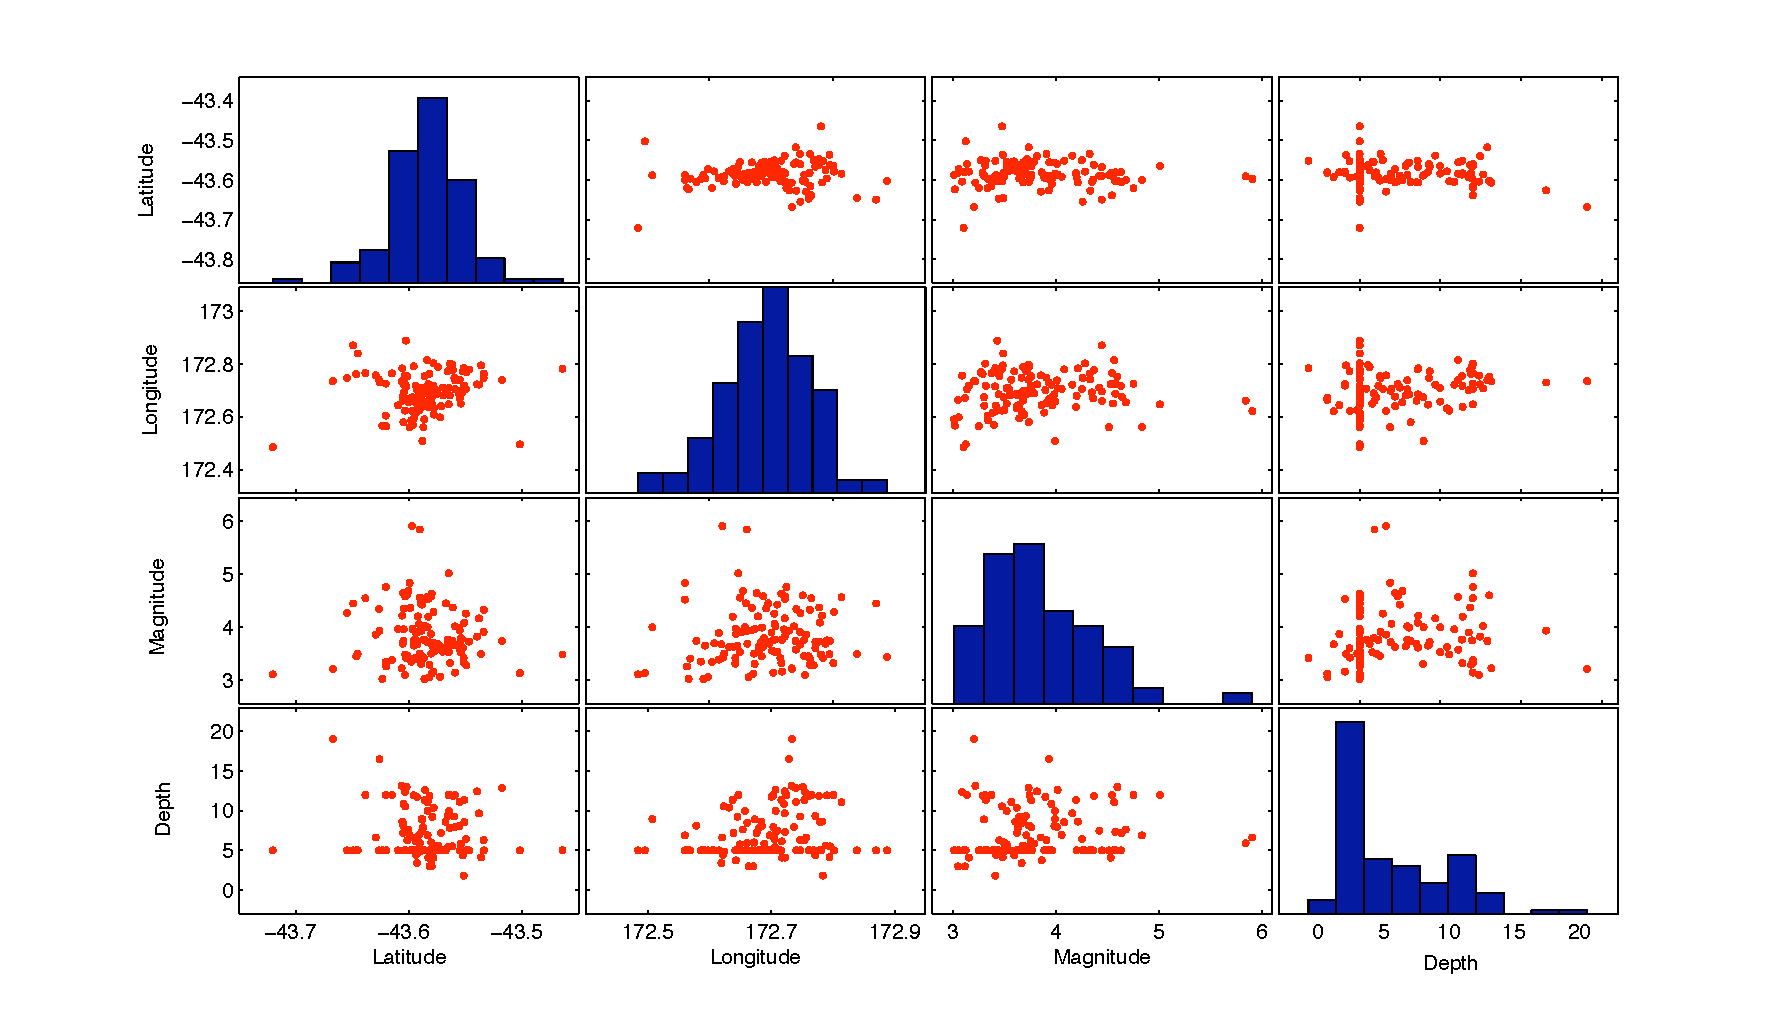
\includegraphics[width=6.5in]{figures/NZEQ20110222ChchLtLnMgDpScatterMatrixPlot}}
\end{figure}


\begin{labwork}\label{LW:NZEQChCch20110222EDA}
Try to understand how to manipulate time stamps of events in \Matlab and the Figures being output by following the comments in the script file {\tt NZEQChCch20110222EDA.m}.
\begin{VrbM}
>> NZEQChCch20110222
ans =   145    14
ans =   145    14
ans =   124    14
ans =   145    14
ans =   145    14
ans =   124    14
ans = 22-Feb-2011 00:00:31
ans = 22-Feb-2011 23:50:01
\end{VrbM}
\VrbMf[label=NZEQChCch20110222EDA.m]{scripts/NZEQChCch20110222EDA.m}
\end{labwork}

\subsubsection{Geostatistical exploratory data analysis with Google Earth}

\begin{figure}[htpb]
\caption{Google Earth Visualisation of the earth quakes\label{F:NZEQ20110222ChchLtLnMgDpInGoogleEarthViewFromUSGS}}
\centering   \makebox{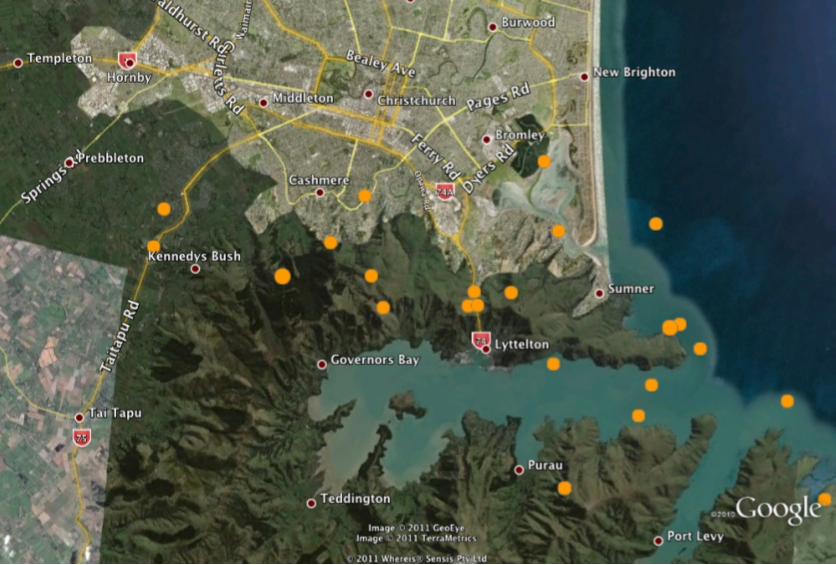
\includegraphics[width=4.5in]{figures/NZEQ20110222ChchLtLnMgDpInGoogleEarthViewFromUSGS}}
\end{figure}

A global search at \href{http://neic.usgs.gov/cgi-bin/epic/epic.cgi}{\url{http://neic.usgs.gov/cgi-bin/epic/epic.cgi}}
%%?SEARCHMETHOD=1&FILEFORMAT=7&SEARCHRANGE=PP&SYEAR=2011&SMONTH=2&SDAY=22&EYEAR=2011&EMONTH=2&EDAY=22&LMAG=&UMAG=&NDEP1=&NDEP2=&IO1=&IO2=&CLAT=0.0&CLON=0.0&CRAD=0.0&SUBMIT=Submit+Search}
with the following parameters:
\begin{verbatim}
Date Range: 2011 2 22 to 2011 2 22
Catalog: USGS/NEIC (PDE-Q)
\end{verbatim}
produced 43 earth quakes world-wide, including those in Christchurch as shown in \hyperref[F:NZEQ20110222ChchLtLnMgDpInGoogleEarthViewFromUSGS]{Figure~\ref*{F:NZEQ20110222ChchLtLnMgDpInGoogleEarthViewFromUSGS}}.  One can do a lot more than a mere visualisation with the USGS/NEIC  database of earth-quakes wolrd-wide, the freely available {\tt Google earth} software bundle \href{http://www.google.com/earth/index.html}{\url{http://www.google.com/earth/index.html}} and the freely available \Matlab package {\tt googleearth} from \href{http://www.mathworks.com/matlabcentral/fx_files/12954/4/content/googleearth/html/html_product_page.html}{\url{http://www.mathworks.com/matlabcentral/fx_files/12954/4/content/googleearth/html/html_product_page.html}}.

\subsection{Metereological Data}

New Zealand's meteorological service NIWA provides weather data under it TERMS AND CONDITIONS FOR ACCESS TO DATA (See \url{http://cliflo.niwa.co.nz/doc/terms_print.html}).  We will explore some data of rainfall and temperatures from NIWA.

\subsubsection{Daily Rainfalls in Christchurch}

%Rainfall Data in Christchurch

Automagic downloading of the data by {\sf Method B} can be done if the data provider allows automated queries.  It can be accomplished by {\tt urlread} for instance.  %Try to download the file



%is being  \work.  But you can t

Paul Brouwers has a basic CliFlo datafeed on \url{http://www.math.canterbury.ac.nz/php/lib/cliflo/rainfall.php}.  %?range=20100425:20100501
This returns the date and rainfall in milli meters as measured from the CHCH aeroclub station. It is assumed that days without readings would not be listed. %It expects a range parameter such as: ?range=20100425:20100501 The first number is the starting search date (YYYYMMDD). Colon as separator. The first number is the ending search date (YYYYMMDD). CliFlo limits us to 2 million rows for the subscription and 40,000 rows per query (which is equivalent of over 100 years of data, so I we're safe -
The data doesn't go back much before 1944.

%wetdataURL = 'http://www.math.canterbury.ac.nz/php/lib/cliflo/?range=20100101:20100510' wetdataURL = 'http://www.math.canterbury.ac.nz/php/lib/cliflo/rainfall.php'
%\work


\begin{labwork}\label{LW:ChchDailyRainfallSince}
Understand how \hyperref[F:ChchDailyRainfallSince]{Figure~\ref*{F:ChchDailyRainfallSince}} is obtained by the script file {\tt RainFallsInChch.m} by typing and following the comments:

\begin{VrbM}
>> RainFallsInChch
RainFallsChch =     [24312x1 int32]    [24312x1 double]
ans =       24312           2
FirstDayOfData =    19430802
LastDayOfData =    20100721
\end{VrbM}

\VrbMf[label=RainFallsInChch.m]{scripts/RainFallsInChch.m}
\end{labwork}

\begin{figure}[htpb]
\caption{Daily rainfalls in Christchurch since March 27 2010 \label{F:ChchDailyRainfallSince}}
\centering   \makebox{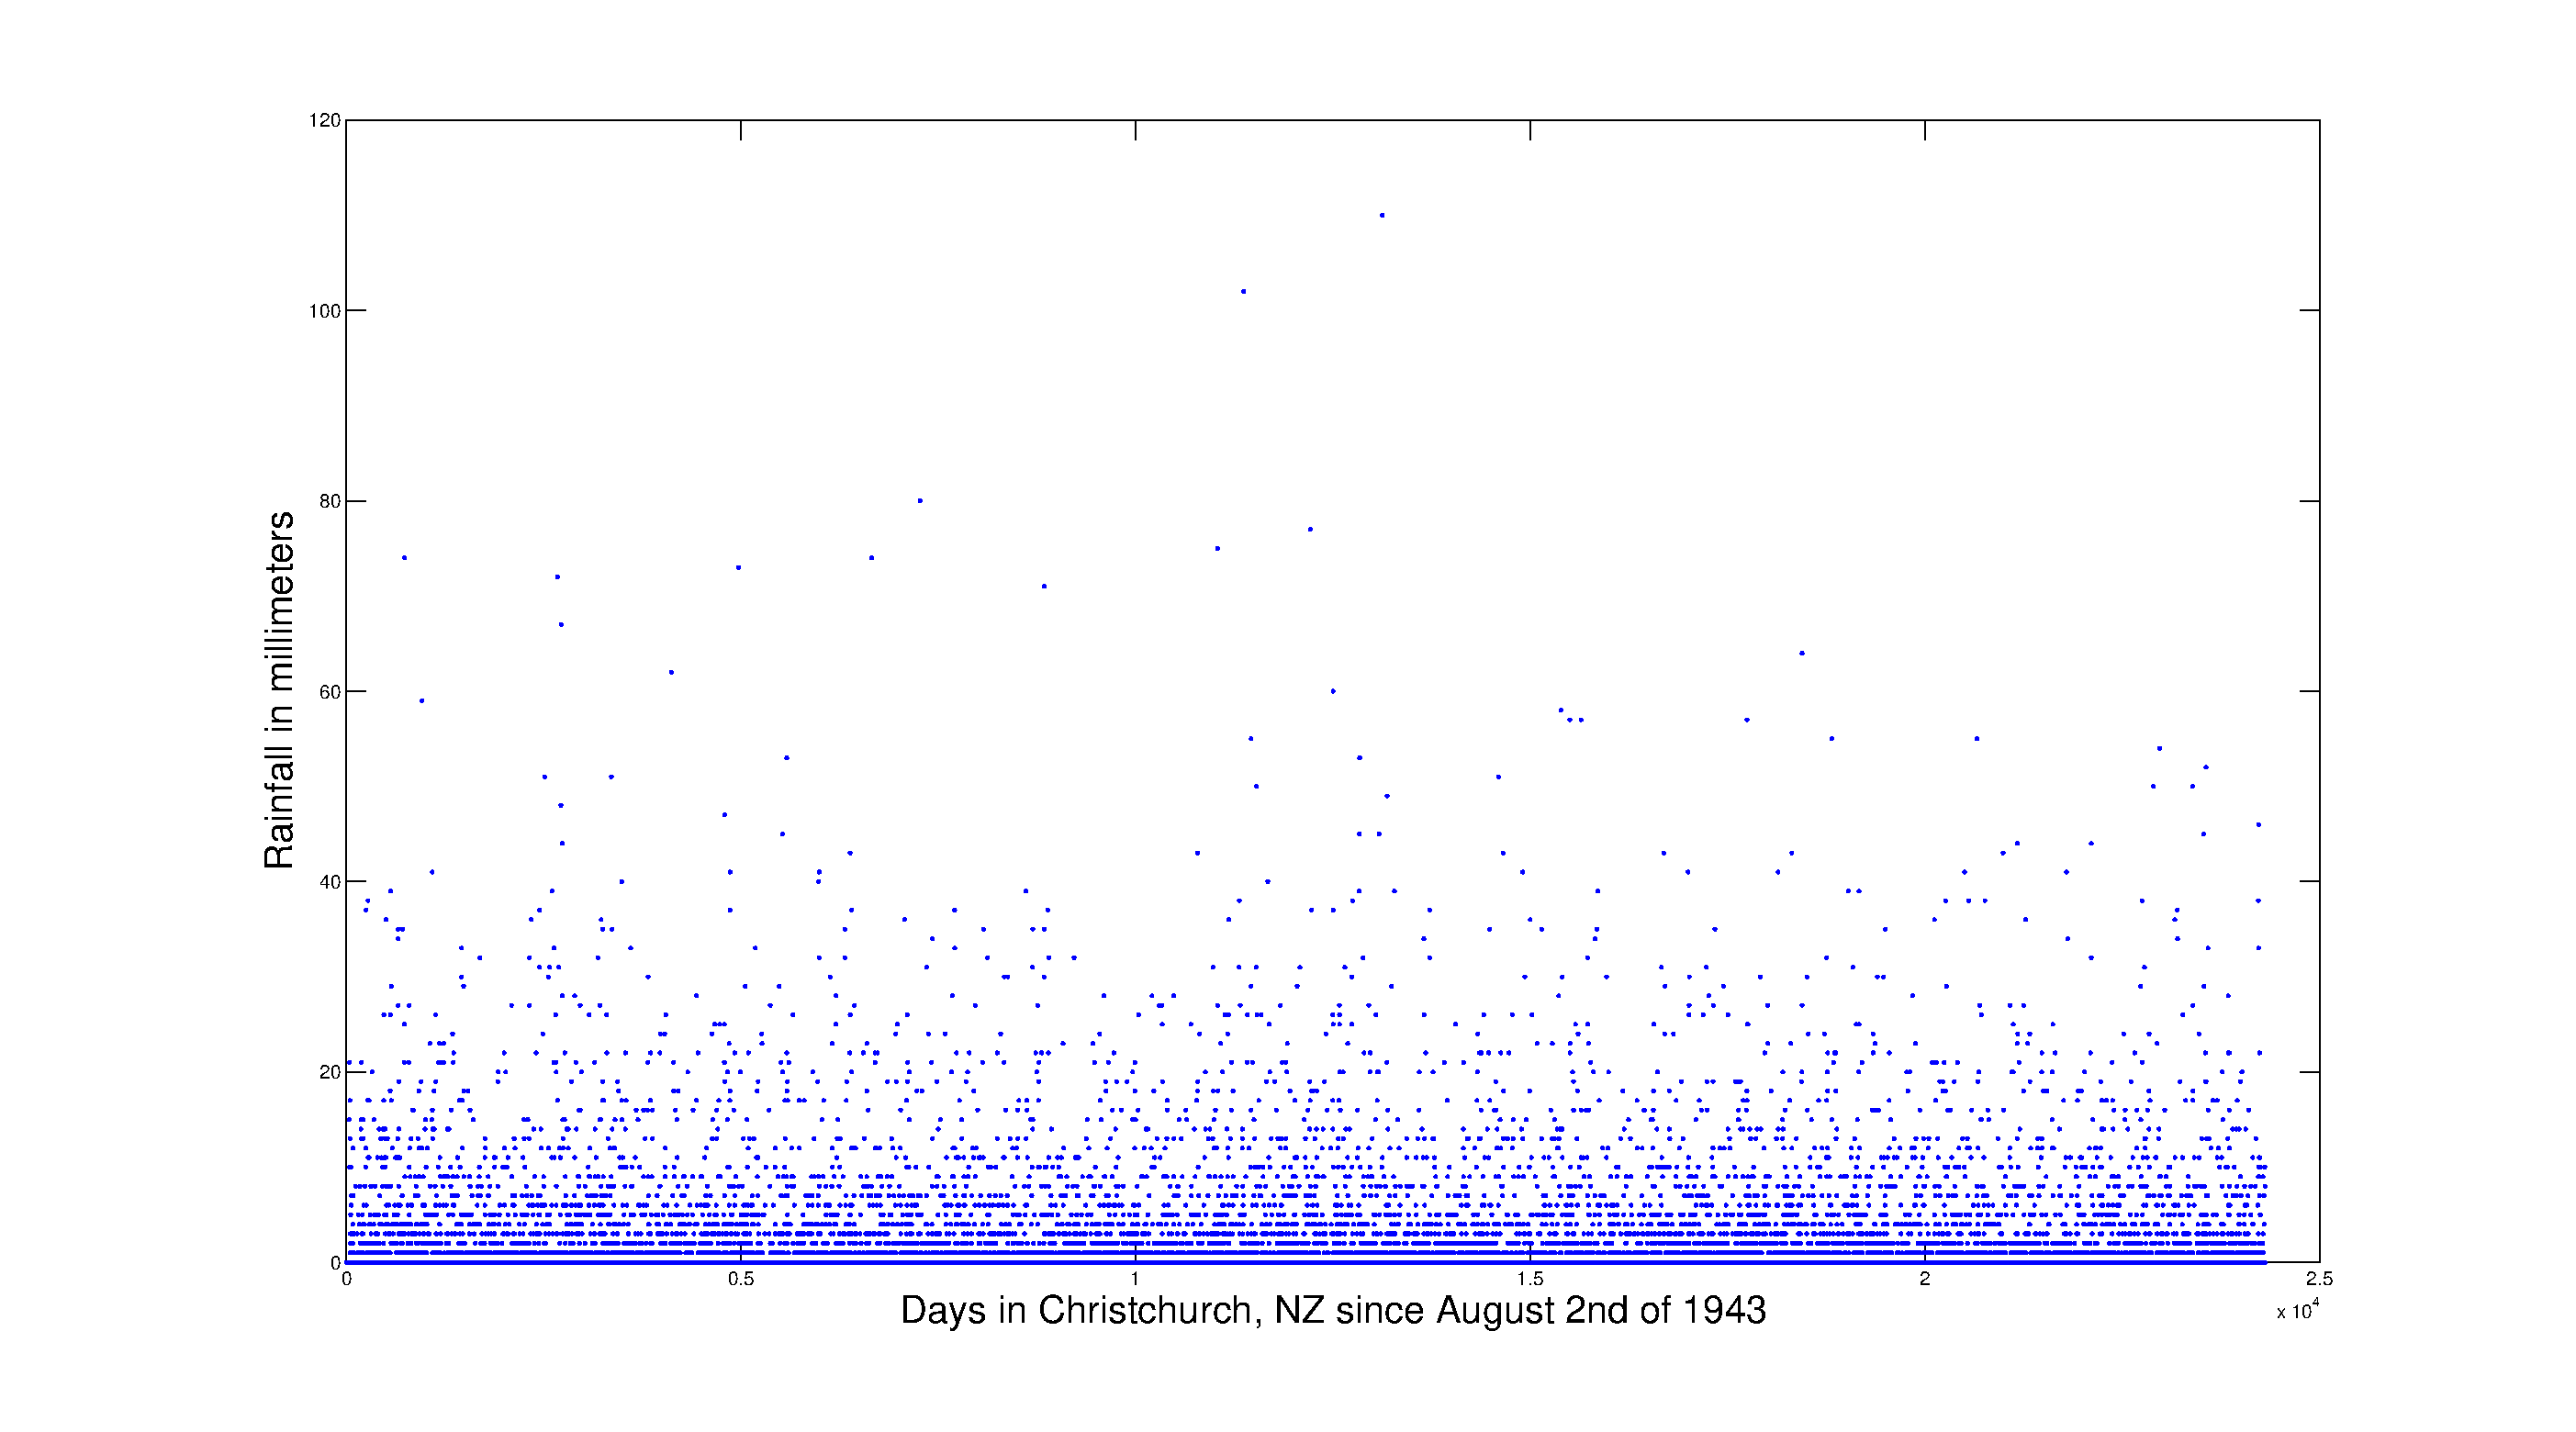
\includegraphics[width=6.5in]{figures/ChchDailyRainfallSince}}
\end{figure}

\subsubsection{Daily Temperatures in Christchurch}


\begin{labwork}\label{LW:ChchTempsLoad}
Understand how \hyperref[F:ChchTemps365DaysSince20100327]{Figure~\ref*{F:ChchTemps365DaysSince20100327}} is being generated by following the comments in the script file {\tt ChchTempsLoad.m} by typing:
\begin{VrbM}
>> ChchTempsLoad
\end{VrbM}
\VrbMf[label=ChchTempsLoad.m]{scripts/ChchTempsLoad.m}
\end{labwork}

\begin{figure}[htpb]
\caption{Daily temperatures in Christchurch for one year since March 27 2010 \label{F:ChchTemps365DaysSince20100327}}
\centering   \makebox{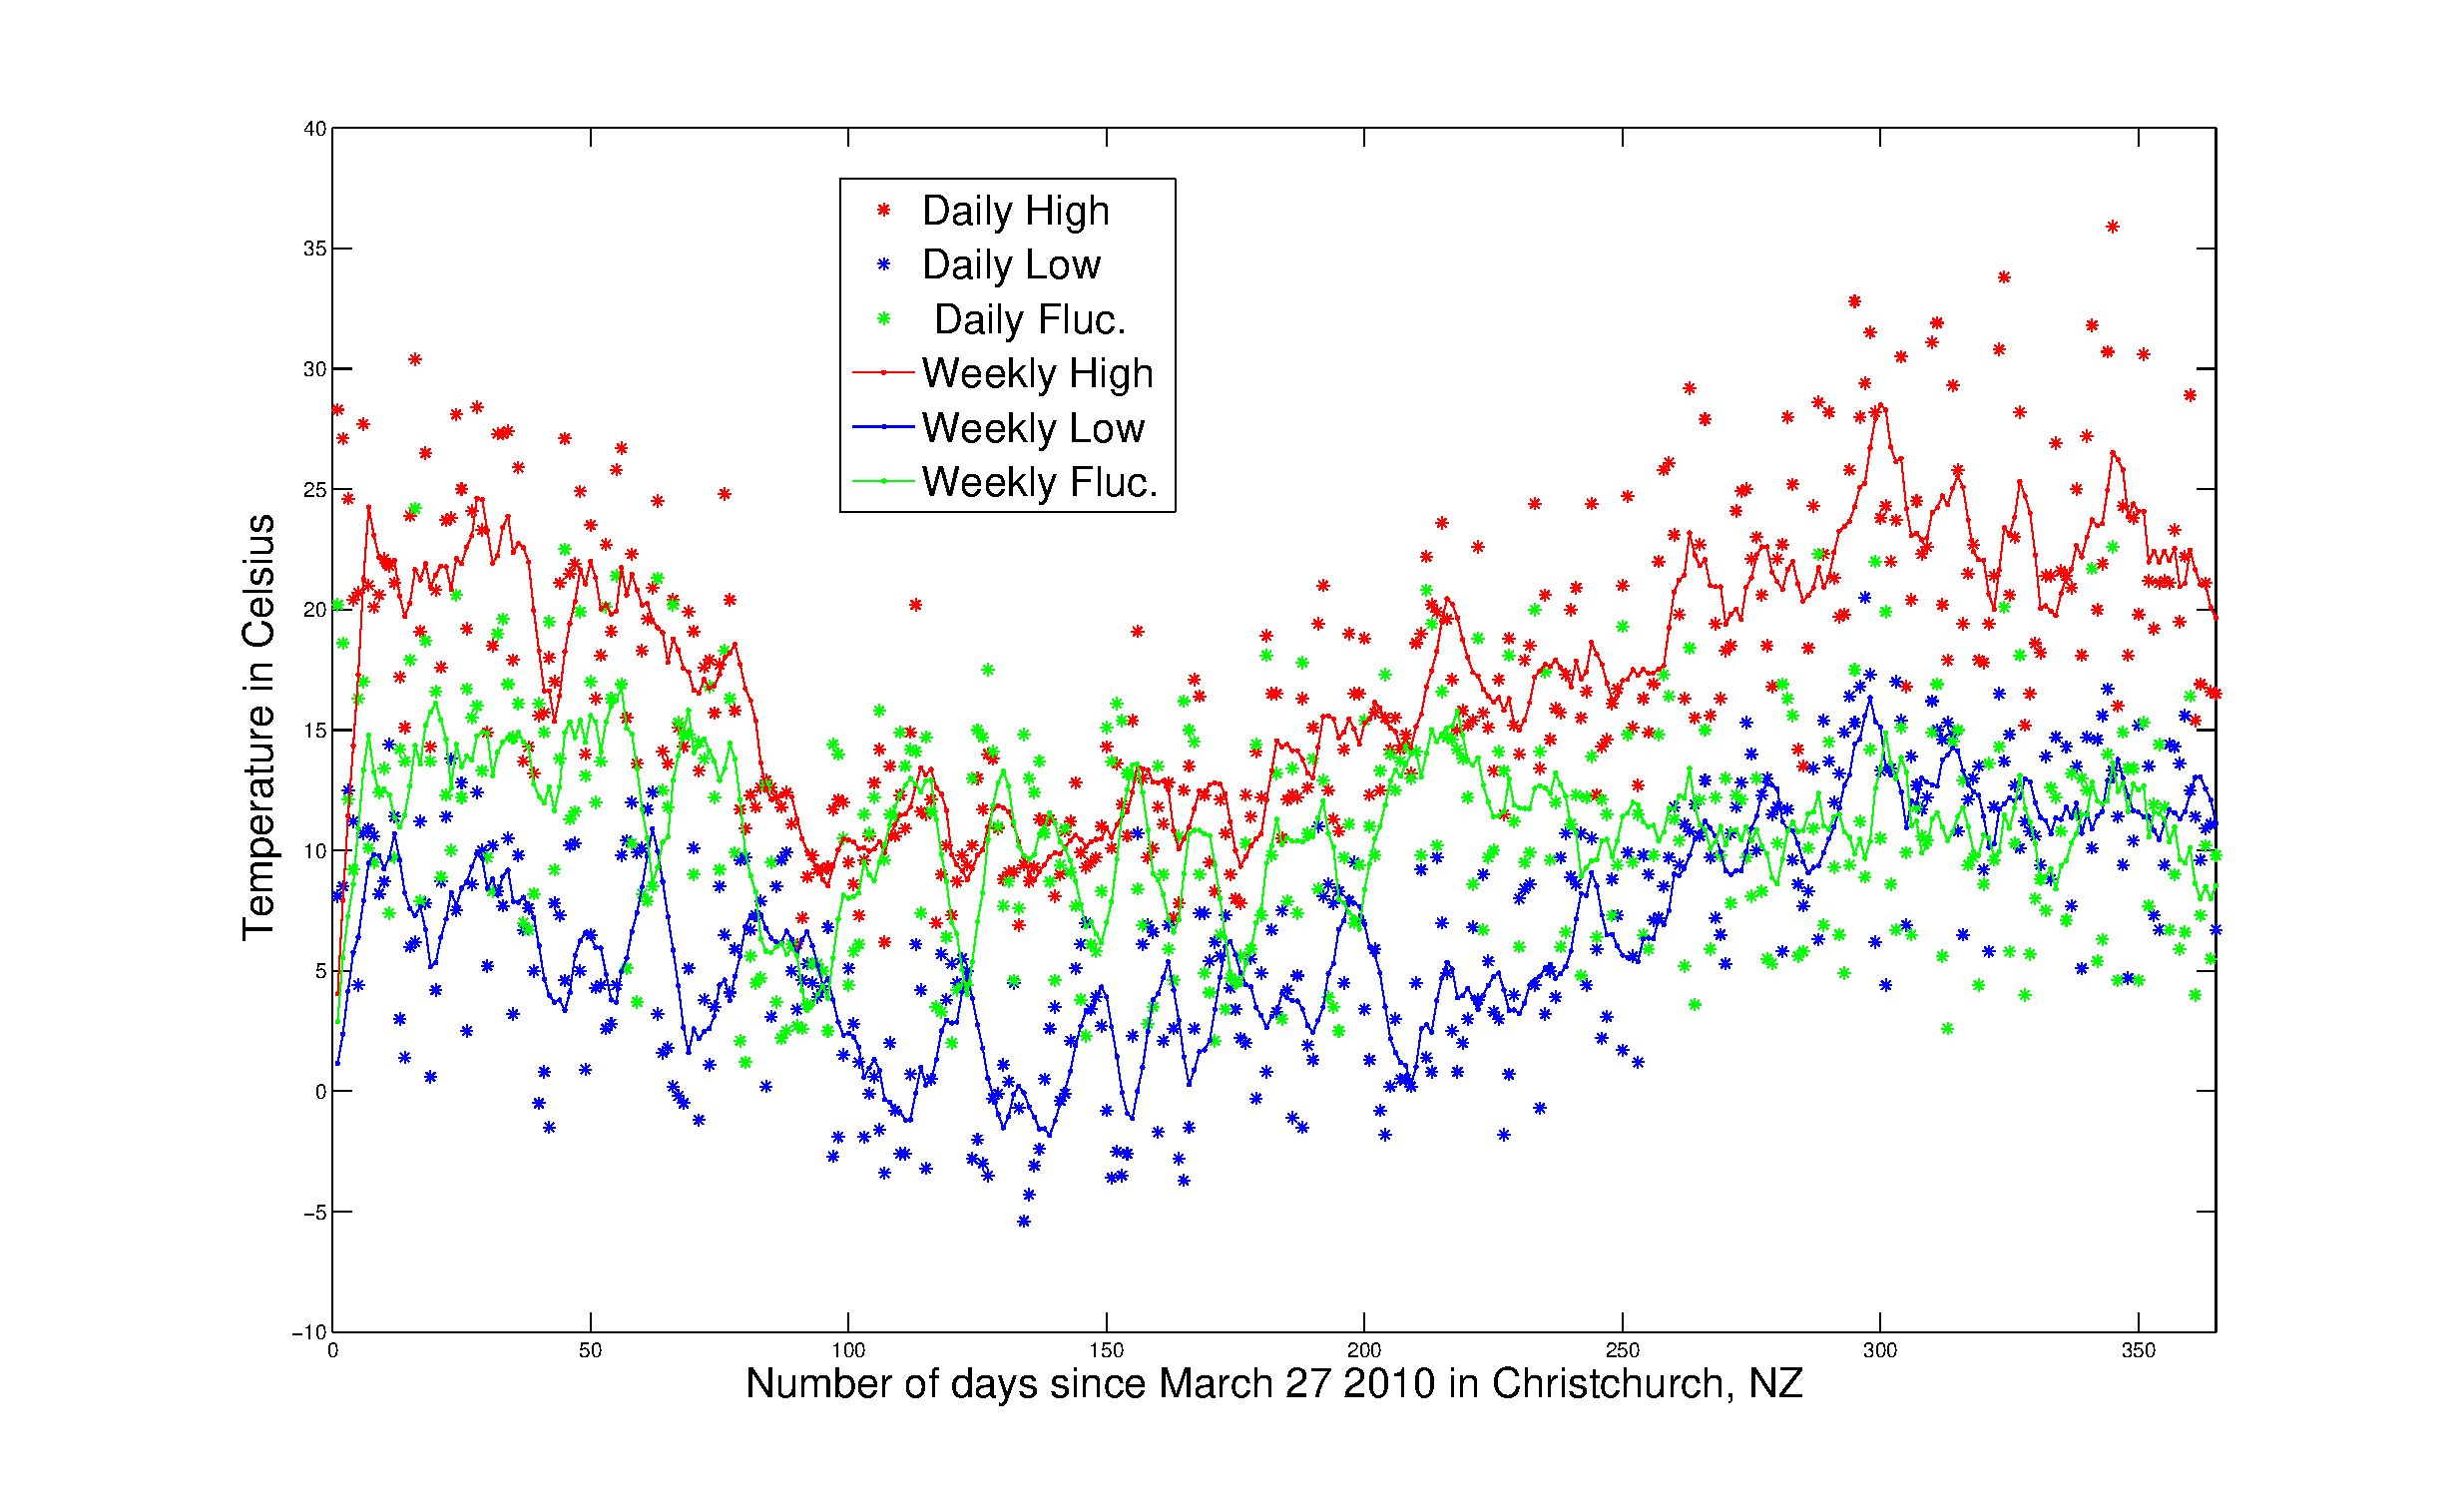
\includegraphics[width=6.5in]{figures/ChchTemps365DaysSince20100327}}
\end{figure}

\subsection{Textual Data}

Processing and analysing textual data to make a decision is another important computational statistical experiment. An obvious example  is machine translation and a less obvious one is exploratory data analysis of the textual content of
\begin{itemize}
\item a large document
\item twitter messages within an online social network of interest
\item etc.
\end{itemize}

An interesting document with a current affairs projection is the Joint Operating Environment 2010 Report by the US Department of Defense.  This document was downloaded from \href{http://www.jfcom.mil/newslink/storyarchive/2010/JOE_2010_o.pdf}{\url{http://www.jfcom.mil/newslink/storyarchive/2010/JOE_2010_o.pdf}}.  The first paragraph of this 74 page document (JOE 2010 Reprort) reads:

{\small
ABOUT THIS STUDY The Joint Operating Environment is intended to inform joint concept development and experimentation throughout the Department of Defense. It provides a perspective on future trends, shocks, contexts, and implications for future joint force commanders and other leaders and professionals in the national security field. This document is speculative in nature and does not suppose to predict what will happen in the next twenty-five years. Rather, it is intended to serve as a starting point for discussions about the future security environment at the operational level of war. Inquiries about the Joint Operating Environment should be directed to USJFCOM Public Affairs, 1562 Mitscher Avenue, Suite 200, Norfolk, VA 23551-2488, (757) 836-6555.

Distribution Statement A: Approved for Public Release
}

\begin{figure}[htpb]
\caption{Wordle of JOE 2010\label{F:joe_vs_wordle}}
\centering   \makebox{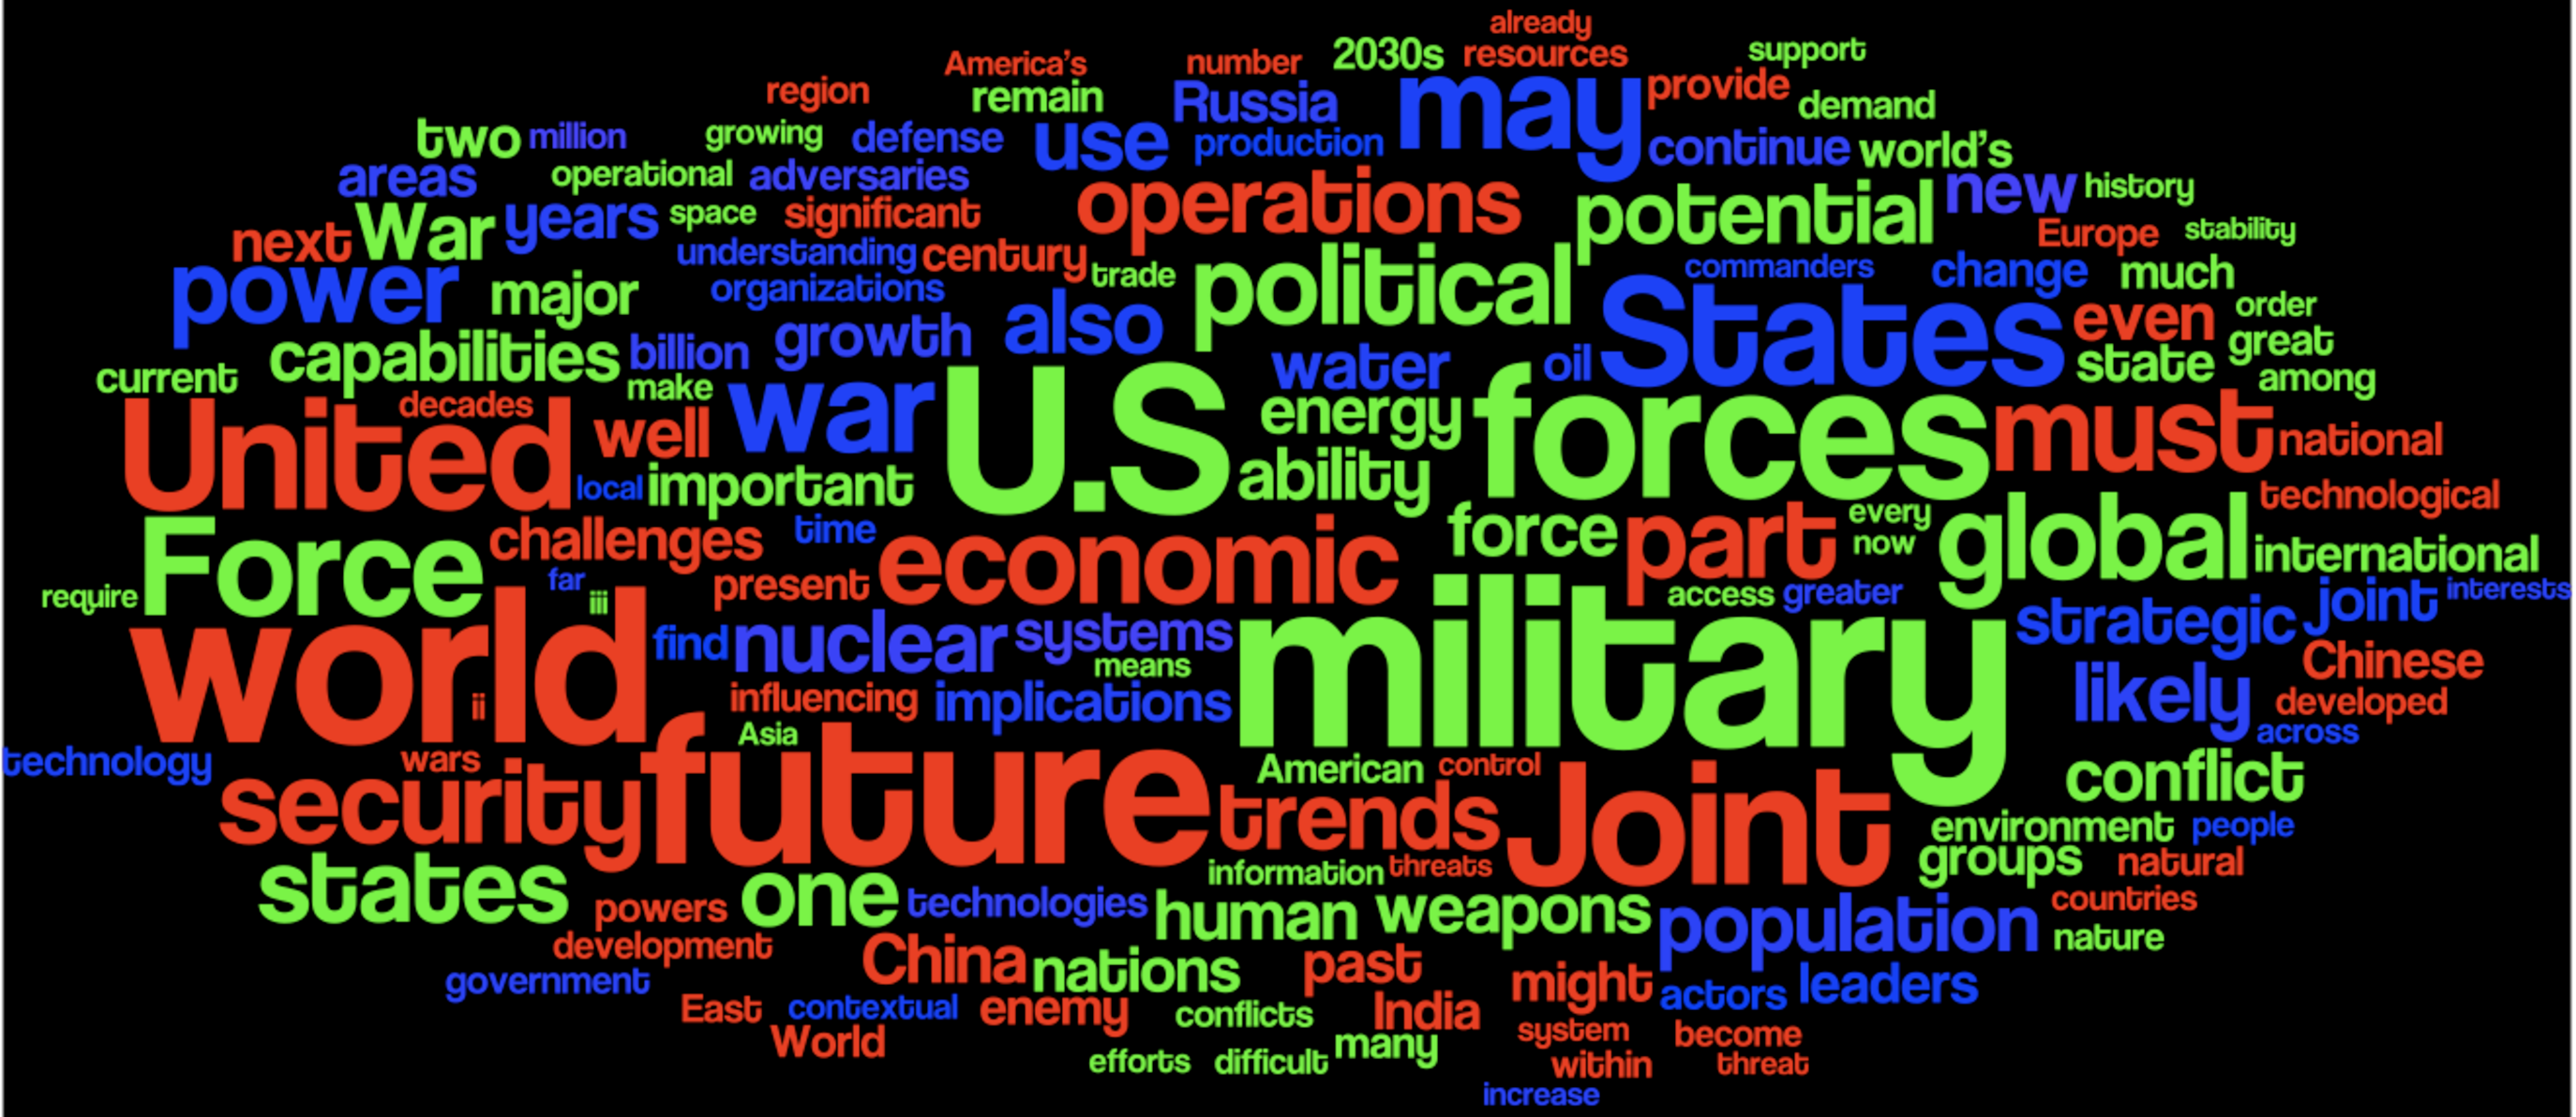
\includegraphics[width=6.5in]{figures/joe_vs_wordle_RaazCroppedPhilWilsonsImage}}
\end{figure}

We can try to produce a statistic of this document by recording the frequency of words in its textual content. Then we can produce a ``word histogram'' or ``word cloud'' to explore the document visually at one of the coarsest possible resolutions of the textual content in the JOE 2010 Report.  The ``word cloud'' shown in \hyperref[F:joe_vs_wordle]{Figure~\ref*{F:joe_vs_wordle}} was produced by Phillip Wilson using {\em wordle} from \href{http://www.wordle.net/}{\url{http://www.wordle.net/}}.  A description from the wordle URL says:

{\small
Wordle is a toy for generating Òword cloudsÓ from text that you provide. The clouds give greater prominence to words that appear more frequently in the source text. You can tweak your clouds with different fonts, layouts, and color schemes. The images you create with Wordle are yours to use however you like. You can print them out, or save them to the Wordle gallery to share with your friends.
}

\begin{labwork}[favourite word cloud]\label{LW:JoeWordle}  This is just for fun.  Produce a ``word cloud'' of your honours thesis or summer project or any other document that fancies your interest by using {\em wordle} from \href{http://www.wordle.net/}{\url{http://www.wordle.net/}}. Play with the aesthetic features to change colour, shapes, etc.\end{labwork}

\subsection{Machine Sensor Data}

Instrumentation of modern machines, such as planes, rockets and cars allow the sensors in the machines to collect live data and dynamically take {\em decisions} and subsequent {\em actions} by executing algorithms to drive their devices in response to the data that is streaming into their sensors.  For example, a rocket may have to adjust its boosters to compensate for the prevailing directional changes in wind in order to keep going up and launch a satellite.
These types of decisions and actions, theorised by {\em controlled Markov processes}, typically arise in various fields of engineering such as, aerospace, civil, electrical, mechanical, robotics, etc.

In an observational setting, without an associated control problem, one can use machine sensor data to get information about some state of the system or phenomenon, i.e., what is it doing? or where is it?, etc.  Sometimes sensors are attached to a sample of individuals from a  wild population, say Emperor Penguins in Antarctica where the phenomenon of interest may be the diving habits of this species after the eggs hatch.  As an other example we can attach sensors to a double pendulum and find what it is doing when we give it a spin.

Based on such observational data the experimenter typically tries to learn about the behaviour of the system from the sensor data to estimate parameters, test hypotheses, etc. Such types of experiments are typically performed by scientists in various fields of science, such as, astronomy, biology, chemistry, geology, physics, etc.

\subsubsection{Chaotic Time Series of a Double Pendulum}

\begin{figure}[htbp]
\begin{center}
{\scriptsize
\begin{tabular}{ccc}
A: DP Schematic & B: Streaming DP data & C: Enclosures of two initially close trajectories\\
  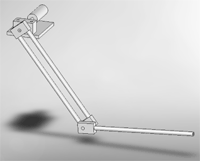
\includegraphics[scale=0.5]{figures/dp} &
  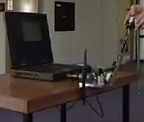
\includegraphics[scale=0.66]{figures/vlcsnap-2010-01-13-10h11m08s38_closeup} &
  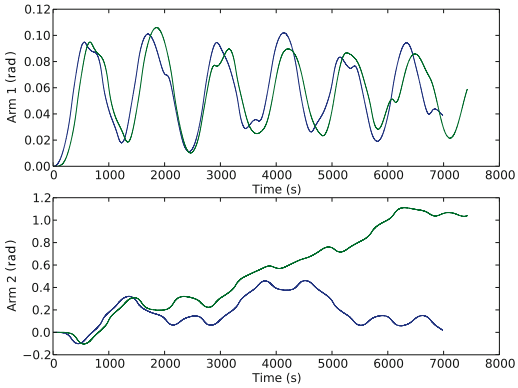
\includegraphics[height=3cm,width=6.75cm]{figures/divergence_piers}
\end{tabular}
}
\end{center}
\caption{Double Pendulum}
\label{F:DP3}
\end{figure}

Sensors called {\em optical encoders} have been attached to the top end of each arm of a chaotic double pendulum in order to obtain the angular position of each arm through time as shown in \hyperref[F:DP3]{Figure~\ref*{F:DP3}}.  Time series of the angular position of each arm for two trajectories that were initialized very similarly, say the angles of each arm of the double pendulum are almost the same at the initial time of release.  Note how quickly the two trajectories diverge!  System with such a sensitivity to initial conditions are said to be {\em chaotic}.

\begin{labwork}[A Challenging Task]\label{LW:DPtrajectoryparsing}  Try this if you are interested.  Read any of the needed details about the design and fabrication of  the double pendulum at \href{http://www.math.canterbury.ac.nz/~r.sainudiin/lmse/double-pendulum/}{\url{http://www.math.canterbury.ac.nz/~r.sainudiin/lmse/double-pendulum/}}.  Then use \Matlab to generate a plot similar to \hyperref[F:DP3]{Figure~\ref*{F:DP3}(C)} using time series data of {\sf trajectory~1} and {\sf  trajectory~2} linked from the bottom of the above URL.
 \end{labwork}

\comment{
\subsection{Biological Data}
\work
}

\section{Exercises in Statistics}\label{S:xsStatistics}
\begin{ExerciseList}
\Exercise What is the sample mean and sample variance of the following dataset:
\[
1, 3, 2, 1, 2, 3, 3
\]
\Answer Apply the formulas for the sample mean, $\overline{X_7}$, and sample variance.
\end{ExerciseList}



%\remove
%%%%%%%%%%%%%%%%%%%%%%%%%%%%%%%%%%%%%%%%%%%%%%%%%%%%%%%%%%%%%%%%%%%%%%%%%%%%%%
%%%% snipped above into csebook

\chapter{Fundamentals of Estimation}
\section{Introduction}
Now that we have been introduced to two notions of convergence for RV sequences, we can begin to appreciate the basic limit theorems used in statistical inference.  The problem of estimation is of fundamental importance in statistical inference and learning.  We will formalise the general estimation problem here.  There are two basic types of estimation.  In point estimation we are interested in estimating a particular point of interest that is supposed to belong to a set of points.  In (confidence) set estimation, we are interested in estimating a set with a particular form that has a specified probability of ``trapping'' the particular point of interest from a set of points.  Here, a point should be interpreted as an element of a collection of elements from some space.

\section{Point Estimation}\label{S:PointEstimation}
{\bf Point estimation} is any statistical methodology that provides one with a ``{\bf single best guess}'' of some specific quantity of interest.  Traditionally, we denote this {\bf quantity of interest as $\theta^*$} and {\bf its point estimate as $\widehat{\theta}$ or $\widehat{\theta}_n$}.  The subscript $n$ in the point estimate $\widehat{\theta}_n$ emphasises that our estimate is based on $n$ observations or data points from a given statistical experiment to estimate $\theta^*$.  This quantity of interest, which is usually unknown, can be: %, namely $\theta$
%, may be an {\bf integral} $\Iz$ of a real valued function $h(x)$, i.e.~$\theta=\Iz := \int_a^b h(x)\,dx \in \Rz$, or simply a 
\begin{itemize}
\item an {\bf integral} $\vartheta^* := \int_A h(x)\,dx \in \BB{\varTheta}$.  If $\vartheta^*$ is finite, then $\BB{\varTheta} =  \Rz$, or %  For e.g.~see \ref{S:BMC} on Monte Carlo integration.
\item a {\bf parameter} $\theta^*$ which is an element of the {\bf parameter space} $\BB{\Theta}$, denoted $\theta^* \in \BB{\Theta}$,
\item a {\bf distribution function (DF)} $F^* \in \Fz := \text{the set of all DFs}$
\item a {\bf density function (pdf)} $f \in \{ \text{``not too wiggly Sobolev functions''} \}$, or 
\item a {\bf regression function} $g^* \in \Gz$, where $\Gz$ is a class of regression functions in a regression experiment with model: $Y=g^*(X)+\epsilon$, such that $\E(\epsilon)=0$, from pairs of observations $\{(X_i,Y_i)\}_{i=1}^n$, or
\item a {\bf classifier} $g^* \in \Gz$, i.e.~a regression experiment with discrete $Y = g^*(X)+\epsilon$, or 
\item a {\bf prediction} in a regression experiment, i.e.~when you want to estimate $Y_i$ given $X_i$. 
\end{itemize}
%\begin{table}[htpb]
%\begin{center}
%\begin{tabular}{|c c c|}
%\hline
%Quantity of Interest $\theta$ & Point Estimation & Sections \\ \hline
%Parameter $\theta \in \BB{\Theta} \subset \Rz^n$ & Parametric Estimation & Section~\ref*{S:ParametricEstimation} \\
%Integral $\Iz := \int_a^bh(x)\,dx$ & Monte Carlo Integration & Section~\ref*{S:BMC} \\ \hline
%\end{tabular}
%\end{center}
%\end{table}

Recall that a statistic is an RV $T(X)$ that maps every data point $x$ in the data space $\Xz$ with $T(x)=t$ in its range $\Tz$, i.e.~$T(x):\Xz \to \Tz$ (\hyperref[D:Statistic]{Definition~\ref*{D:Statistic}}).  Next, we look at a specific class of statistics whose range is the parameter space $\BB{\Theta}$.
\begin{definition}[Point Estimator]\label{D:Estimator}
A {\bf point estimator} $\widehat{\Theta}$ of some {\bf fixed and possibly unknown} $\theta^* \in \BB{\Theta}$ is a statistic that associates each data point $x \in \Xz$ with an estimate $\widehat{\Theta}(x)=\widehat{\theta} \in \BB{\Theta}$,  
\[
\boxed{
 \widehat{\Theta} := \widehat{\Theta}(x)=\widehat{\theta}: \Xz \to \BB{\Theta}
 } \ .
\]
If our data point $x := (x_1,x_2,\ldots,x_n)$ is an $n$-vector or a point in the $n$-dimensional real space, i.e.~$x := (x_1,x_2,\ldots,x_n) \in \Xz_n \subset \Rz^n$, then we emphasise the dimension $n$ in our point estimator $\widehat{\Theta}_n$ of $\theta^* \in \BB{\Theta}$.
\[
\boxed{
\widehat{\Theta}_n :=  \widehat{\Theta}_n(x:=(x_1,x_2,\ldots,x_n))=\widehat{\theta}_n : \Xz_n \to \BB{\Theta}, \quad \Xz_n \subset \Rz^n 
} \ .
\]
 The typical situation for us involves point estimation of $\theta^* \in \BB{\Theta}$ on the basis of one realisation $x \in\Xz_n \subset \Rz^n$ of an independent and identically distributed (IID) random vector $X=(X_1,X_2,\ldots,X_n)$, such that $X_1,X_2,\ldots,X_n \overset{\IID}{\sim} X_1$ and the DF of $X_1$ is $F(x_1; \theta^*)$, i.e.~the distribution of the IID RVs, $X_1, X_2,\ldots,X_n$, is parameterised by $\theta^* \in \BB{\Theta}$.
\end{definition}

\begin{example}[Coin Tossing Experiment ($X_1,\ldots,X_n \overset{IID}{\sim} \bernoulli(\theta^*)$)]\label{EX:CoinTossing}
I tossed a coin that has an unknown probability $\theta^*$ of landing Heads independently and identically $10$ times in a row.  Four of my outcomes were Heads and the remaining six were Tails, with the actual sequence of Bernoulli outcomes (Heads $\to 1$ and Tails $\to 0$) being $(1,0,0,0,1,1,0,0,1,0)$.  I would like to estimate the probability $\theta^* \in \BB{\Theta} = [0,1]$ of observing Heads using the natural estimator $\widehat{\Theta}_n((X_1,X_2,\ldots,X_n))$ of $\theta^*$:
\[
\widehat{\Theta}_n((X_1,X_2,\ldots,X_n)) := \widehat{\Theta}_n = \frac{1}{n} \sum_{i=1}^n X_i =: \overline{X}_n
\]
For the coin tossing experiment I just performed ($n=10$ times), the point estimate of the unknown $\theta^*$ is:
\begin{eqnarray}
\widehat{\theta}_{10} = \widehat{\Theta}_{10}((x_1,x_2,\ldots,x_{10})) 
&=&\widehat{\Theta}_{10}((1,0,0,0,1,1,0,0,1,0)) \notag \\
&=& \frac{1+0+0+0+1+1+0+0+1+0}{10}=\frac{4}{10}=0.40 \notag \ .
\end{eqnarray}
\end{example}

\begin{labwork}[$\bernoulli(38/75)$ Computer Experiment]\label{LW:1000CoinTossingExp}
Simulate one thousand IID samples from a $\bernoulli(\theta^*=38/75)$ RV and store this data in an array called $\tt Samples$.  Use your student ID to initialise the fundamental sampler.  Now, pretend that you don't know the true $\theta^*$ and estimate $\theta^*$ using our estimator $\widehat{\Theta}_n=\overline{X}_n$ from the data array $\tt Samples$ for each sample size $n=1,2,\ldots,1000$.  Plot the one thousand estimates $\widehat{\theta}_1,\widehat{\theta}_2,\ldots,\widehat{\theta}_{1000}$ as a function of the corresponding sample size.  Report your observations regarding the behaviour of our estimator as the sample size increases.
\end{labwork}

\section{Some Properties of Point Estimators}\label{S:PropPointEstim}
Given that an estimator is merely a function from the data space to the parameter space, we need choose only the best estimators available.  Recall that a point estimator $\widehat{\Theta}_n$, being a statistic or an RV of the data has a probability distribution over its range $\BB{\Theta}$.  This distribution over $\BB{\Theta}$ is called the {\bf sampling distribution} of $\widehat{\Theta}_n$.  Note that the sampling distribution not only depends on the statistic $\widehat{\Theta}_n := \widehat{\Theta}_n(X_1,X_2,\ldots,X_n)$ but also on $\theta^*$ which in turn determines the distribution of the IID data vector $(X_1,X_2,\ldots,X_n)$.  The following definitions are useful for selecting better estimators from some lot of them.

\begin{definition}[Bias of a Point Estimator]\label{D:Bias}
The $\mathsf{bias}_n$ of an estimator $\widehat{\Theta}_n$ of  $\theta^* \in \BB{\Theta}$ is:
\begin{equation}\label{E:Bias}
\boxed{
\mathsf{bias}_n=\mathsf{bias}_n(\widehat{\Theta}_n) := \E_{\theta^*}(\widehat{\Theta}_n) - \theta^* = \int_{\Xz_n} \widehat{\Theta}_n(x) \, dF(x;\theta^*) - \theta^*
}
 \ .
\end{equation} 
We say that the estimator $\widehat{\Theta}_n$ is {\bf unbiased} if $\mathsf{bias}_n(\widehat{\Theta}_n)=0$ or if $\E_{\theta^*}(\widehat{\Theta}_n)=\theta^*$ for every $n$.  If $\lim_{n \to \infty}\mathsf{bias}_n(\widehat{\Theta}_n)=0$, we say that the estimator is {\bf asymptotically unbiased}.
\end{definition}
Since the expectation of the sampling distribution of the point estimator $\widehat{\Theta}_n$ depends on the unknown $\theta^*$, we emphasise the $\theta^*$-dependence by $\E_{\theta^*}(\widehat{\Theta}_n)$.

\begin{example}[Bias of our Estimator of $\theta^*$]\label{EX:BiasEstimatePFromNIIDBernoulliTrials}
Consider the sample mean estimator $\widehat{\Theta}_n := \overline{X}_n$ of $\theta^*$, from $X_1,X_2,\ldots,X_n \overset{\IID}{\sim} \bernoulli(\theta^*)$.  That is, we take the sample mean of the $n$ IID $\bernoulli(\theta^*)$ trials to be our point estimator of $\theta^*\in[0,1]$.  Then, {\bf this estimator is unbiased} since:
\[
\E_{\theta^*}(\widehat{\Theta}_n) = \E_{\theta^*} \left( n^{-1} \sum_{i=1}^n X_i \right) = n^{-1} \E_{\theta^*} \left(  \sum_{i=1}^n X_i \right) = n^{-1} \sum_{i=1}^n \E_{\theta^*}(X_i) = n^{-1} n \theta^* = \theta^* \ .
\]
\end{example}

\begin{definition}[Standard Error of a Point Estimator]
The standard deviation of the point estimator $\widehat{\Theta}_n$ of  $\theta^* \in \BB{\Theta}$ is called the {\bf standard error}:
\begin{equation}\label{E:se}
\boxed{
\mathsf{se}_n = \mathsf{se}_n(\widehat{\Theta}_n)=\sqrt{\V_{\theta^*}(\widehat{\Theta}_n)} = \sqrt{ \int_{\Xz_n} \left( \widehat{\Theta}_n(x) - \E_{\theta^*}(\widehat{\Theta}_n) \right)^2 \, dF(x;\theta^*)}
}\ .
\end{equation}
\end{definition}
Since the variance of the sampling distribution of the point estimator $\widehat{\Theta}_n$ depends on the fixed and possibly unknown $\theta^*$, as emphasised by $\V_{\theta^*}$ in \eqref{E:se}, the $\mathsf{se}_n$ is also a possibly unknown quantity and may itself be estimated from the data.  The estimated standard error, denoted by $\widehat{\mathsf{se}}_n$, is calculated by replacing $\V_{\theta^*}(\widehat{\Theta}_n)$ in \eqref{E:se} with its appropriate estimate.

\begin{example}[Standard Error of our Estimator of $\theta^*$]\label{EX:StdErrEstimatePFromNIIDBernoulliTrials}
Consider the sample mean estimator $\widehat{\Theta}_n := \overline{X}_n$ of $\theta^*$, from $X_1,X_2,\ldots,X_n \overset{\IID}{\sim} \bernoulli(\theta^*)$.  Observe that the statistic: 
$$T_n((X_1,X_2,\ldots,X_n)) := n \,  \widehat{\Theta}_n((X_1,X_2,\ldots,X_n)) = \sum_{i=1}^n X_i$$ is the $\binomial(n,\theta^*)$ RV.
The standard error  $\mathsf{se}_n$ of this estimator is:
\[
\mathsf{se}_n=\sqrt{\V_{\theta^*}(\widehat{\Theta}_n)}
= \sqrt{\V_{\theta^*}\left(\sum_{i=1}^n \frac{X_i}{n} \right)}
= \sqrt{\left(\sum_{i=1}^n \frac{1}{n^2}\V_{\theta^*}(X_i) \right)}
= \sqrt{\frac{n}{n^2}\V_{\theta^*}(X_i)}
=\sqrt{{\theta^*}(1-{\theta^*})/n} \ .
\]
\end{example}

Another reasonable property of an estimator is that it converge to the ``true'' parameter $\theta^*$ -- here ``true'' means the supposedly fixed and possibly unknown $\theta^*$, as we gather more and more IID data from a $\theta^*$-specified DF $F(x; \theta^*)$.  This property is stated precisely next.
\begin{definition}[Asymptotic Consistency of a Point Estimator]\label{D:Consistency}
A point estimator $\widehat{\Theta}_n$ of $\theta^* \in \BB{\Theta}$ is said to be {\bf asymptotically consistent} if:
\[
\boxed{
\widehat{\Theta}_n \overset{P}{\longrightarrow} \theta^*
} \qquad \text{i.e., for any real $\epsilon > 0$,} \quad
\boxed{
\lim_{n \to \infty} \P (| \widehat{\Theta}_n - \theta^* | > \epsilon) = 0
} \ .
\]
\end{definition}

\begin{definition}[Mean Squared Error (MSE) of a Point Estimator]\label{D:MSE}
Often, the quality of a point estimator $\widehat{\Theta}_n$ of $\theta^* \in \BB{\Theta}$ is assessed by the {\bf mean squared error} or $\mathsf{MSE}_n$ defined by:
\begin{equation}\label{E:MSE}
\boxed{
\mathsf{MSE}_n=\mathsf{MSE}_n(\widehat{\Theta}_n) := \E_{\theta^*} \left((\widehat{\Theta}_n-\theta^*)^2 \right) 
= \int_{\Xz} (\widehat{\Theta}_n(x)-\theta^*)^2 \, dF(x;\theta^*) 
} \ .
\end{equation}
\end{definition}

The following proposition shows a simple relationship between the mean square error, bias and variance of an estimator $\widehat{\Theta}_n$ of $\theta^*$.
\begin{prop}[The $\sqrt{\mathsf{MSE}_n}:\mathsf{se}_n:\mathsf{bias}_n$--Sided Right Triangle of an Estimator]
Let $\widehat{\Theta}_n$ be an estimator of $\theta^* \in \BB{\Theta}$.  Then:
\begin{equation}\label{E:RMseSeBiasTriangle}
\boxed{
\mathsf{MSE}_n(\widehat{\Theta}_n) 
= (\mathsf{se}_n(\widehat{\Theta}_n))^2 + (\mathsf{bias}_n(\widehat{\Theta}_n))^2
} \ .
\end{equation}
{\scriptsize
\begin{proof}
\begin{eqnarray}
& & LHS \notag \\
&=& \mathsf{MSE}_n(\widehat{\Theta}_n) \notag \\
&:=& \E_{\theta^*} \left((\widehat{\Theta}_n-\theta^*)^2 \right), \qquad  \text{by definition of $\mathsf{MSE}_n$ \eqref{E:MSE}} \notag \\
&=& \E_{\theta^*} \left( \left( \ \underset{A}{\underbrace{\left(\widehat{\Theta}_n -\E_{\theta^*}(\widehat{\Theta}_n) \right)}} + \underset{B}{\underbrace{\left(\E_{\theta^*}(\widehat{\Theta}_n) -\theta^* \right)}} \ \right)^2 \right), \qquad \text{by subtracting and adding the constant $\E_{\theta^*}(\widehat{\Theta}_n)$} \notag \\
&=& \E_{\theta^*} \left( \underset{A^2}{\underbrace{{\left(\widehat{\Theta}_n -\E_{\theta^*}(\widehat{\Theta}_n) \right)}^2}} + \underset{2AB}{\underbrace{2  {\left(\widehat{\Theta}_n -\E_{\theta^*}(\widehat{\Theta}_n) \right)} {\left(\E_{\theta^*}(\widehat{\Theta}_n) -\theta^* \right)}}} + \underset{B^2}{\underbrace{{\left(\E_{\theta^*}(\widehat{\Theta}_n) -\theta^* \right)}^2}}  \right), \qquad \text{$\because \ (A+B)^2=A^2+2AB+B^2$} \notag \\
&=& \E_{\theta^*} \left( {\left(\widehat{\Theta}_n -\E_{\theta^*}(\widehat{\Theta}_n) \right)}^2 \right) + 
\E_{\theta^*} \left( 2  {\left(\widehat{\Theta}_n -\E_{\theta^*}(\widehat{\Theta}_n) \right)} {\left(\E_{\theta^*}(\widehat{\Theta}_n) -\theta^* \right)} \right) + 
\E_{\theta^*} \left( {\left(\E_{\theta^*}(\widehat{\Theta}_n) -\theta^* \right)}^2  \right), %\quad \text{taking $\E_{\theta^*}(\cdot)$ of $A^2$, $2AB$ and $B^2$} 
\notag \\
&=& \E_{\theta^*} \left( {\left(\widehat{\Theta}_n -\E_{\theta^*}(\widehat{\Theta}_n) \right)}^2 \right) + 
\underset{C}{\underbrace{2 {\left(\E_{\theta^*}(\widehat{\Theta}_n) -\theta^* \right)}}} \underset{D}{\underbrace{ \E_{\theta^*} \left(  {\left(\widehat{\Theta}_n -\E_{\theta^*}(\widehat{\Theta}_n) \right)} \right)}} + 
\E_{\theta^*} \left( {\left(\E_{\theta^*}(\widehat{\Theta}_n) -\theta^* \right)}^2  \right), \quad \text{$\because \ C$ 
% := 2 {\left(\E_{\theta^*}(\widehat{\Theta}_n) -\theta^* \right)}$
is constant} \notag \\
&=& \E_{\theta^*} \left( {\left(\widehat{\Theta}_n -\E_{\theta^*}(\widehat{\Theta}_n) \right)}^2 \right) + 
0 + 
\E_{\theta^*} \left( {\left(\E_{\theta^*}(\widehat{\Theta}_n) -\theta^* \right)}^2  \right), \qquad \text{$\because \ D := \E_{\theta^*} \left(  {\left(\widehat{\Theta}_n -\E_{\theta^*}(\widehat{\Theta}_n) \right)} \right)=\E_{\theta^*}(\widehat{\Theta}_n ) - \E_{\theta^*}(\widehat{\Theta}_n) = 0$} \notag \\
&=& \V_{\theta^*}(\widehat{\Theta}_n)+ 
\E_{\theta^*} \left( {\left(\E_{\theta^*}(\widehat{\Theta}_n) -\theta^* \right)}^2  \right), \qquad \text{$\because \ \V_{\theta^*}(\widehat{\Theta}_n) := \E_{\theta^*} \left( {\left(\widehat{\Theta}_n -\E_{\theta^*}(\widehat{\Theta}_n) \right)}^2 \right)$, by definition of variance} \notag \\
&=& \left( \sqrt{\V_{\theta^*}(\widehat{\Theta}_n)} \right)^2+ 
\E_{\theta^*} \left( {\left( \mathsf{bias}_n(\widehat{\Theta}_n) \right)}^2  \right), \qquad \text{$\because \  \mathsf{bias}_n(\widehat{\Theta}_n) = \E_{\theta^*}(\widehat{\Theta}_n) -\theta^* $, by definition of $\mathsf{bias}_n$ of an estimator $\widehat{\Theta}_n$} \notag \\
&=&  \left(  \mathsf{se}_n(\widehat{\Theta}_n) \right)^2 + 
\E_{\theta^*} \left( {\left( \mathsf{bias}_n(\widehat{\Theta}_n) \right)}^2  \right) , \qquad 
\text{$\because \ \mathsf{se}_n(\widehat{\Theta}_n) := \sqrt{\V_{\theta^*}(\widehat{\Theta}_n)}$, by definition \eqref{E:se}} \notag \\
&=&  \left(  \mathsf{se}_n(\widehat{\Theta}_n) \right)^2 + 
 {\left( \mathsf{bias}_n(\widehat{\Theta}_n) \right)}^2, \qquad 
\text{$\because \  \mathsf{bias}_n(\widehat{\Theta}_n) = \E_{\theta^*}(\widehat{\Theta}_n) -\theta^*$ and $\left( \mathsf{bias}_n(\widehat{\Theta}_n) \right)^2$ are constants.} \notag \\
&=& RHS \notag 
\end{eqnarray}
\end{proof}
}
\end{prop}

\begin{prop}[Asymptotic consistency of a point estimator]\label{P:AsympConsistencyUnbiasedSE0}
Let $\widehat{\Theta}_n$ be an estimator of $\theta^* \in \BB{\Theta}$.  Then, if $\mathsf{bias}_n(\widehat{\Theta}_n) \to 0$ and $\mathsf{se}_n(\widehat{\Theta}_n) \to 0$ as $n \to \infty$, the estimator $\widehat{\Theta}_n$ is asymptotically consistent:
\[
\widehat{\Theta}_n \overset{P}{\longrightarrow} \theta^* \ .
\]
{\scriptsize
\begin{proof}
If $\mathsf{bias}_n(\widehat{\Theta}_n) \to 0$ and $\mathsf{se}_n(\widehat{\Theta}_n) \to 0$, then by \eqref{E:RMseSeBiasTriangle}, $\mathsf{MSE}_n(\widehat{\Theta}_n) \to 0$, i.e.~that $\E_{\theta^*}\left( (\widehat{\Theta}_n-\theta^*)^2 \right) \to 0$.  This type of convergence of the RV $\widehat{\Theta}_n$ to the $Point~Mass(\theta^*)$ RV as $n \to \infty$ is called convergence in {\bf quadratic mean} or {\bf convergence in} $\B{L_2}$ and denoted by $\widehat{\Theta}_n \overset{qm}{\longrightarrow} \theta^*$.  Convergence in quadratic mean is a stronger notion of convergence than convergence in probability, in the sense that 
\[
\E_{\theta^*}\left( (\widehat{\Theta}_n-\theta^*)^2 \right) \to 0 \quad \text{ or } \quad \widehat{\Theta}_n \overset{qm}{\longrightarrow} \theta^* \implies \widehat{\Theta}_n \overset{P}{\longrightarrow} \theta^* \ .
\]
Thus, if we prove the above implication we are done with the proof of our proposition.  To show that convergence in quadratic mean implies convergence in probability for general sequence of RVs $X_n$ converging to an RV $X$, we first assume that $X_n \overset{qm}{\longrightarrow} X$.
Now, fix any $\epsilon>0$.  Then by Markov's inequality \eqref{E:MarkovNeq},
\[
\P(|X_n-X|>\epsilon) = \P(|X_n-X|^2>\epsilon^2) \leq \frac{\E(|X_n-X|^2)}{\epsilon^2} \to 0 \ ,
\]
and we have shown that the definition of convergence in probability holds provided convergence in quadratic mean holds.
\end{proof}
}
\end{prop}
We want our estimator to be unbiased with small standard errors as the sample size $n$ gets large.  The {\bf point estimator} $\widehat{\Theta}_n$ will then produce a {\bf point estimate} $\widehat{\theta}_n$:
$$\widehat{\Theta}_n((x_1,x_2,\ldots,x_n)) = \widehat{\theta}_n \in \BB{\Theta} \enspace ,$$ on the basis of the {\bf observed data} $(x_1,x_2,\ldots,x_n)$, that is close to the {\bf true parameter} $\theta^* \in \BB{\Theta}$.

\begin{example}[Asymptotic consistency of our Estimator of $\theta^*$]
Consider the sample mean estimator $\widehat{\Theta}_n := \overline{X}_n$ of $\theta^*$, from $X_1,X_2,\ldots,X_n \overset{\IID}{\sim} \bernoulli(\theta^*)$.  Since $\mathsf{bias}_n(\widehat{\Theta}_n)=0$ for any $n$ and 
$\mathsf{se}_n=\sqrt{\theta^*(1-\theta^*)/n} \to 0$, as $n \to \infty$, by 
\hyperref[P:AsympConsistencyUnbiasedSE0]{Proposition \ref*{P:AsympConsistencyUnbiasedSE0}}, 
$\widehat{\Theta}_n \overset{P}{\longrightarrow} \theta^*$.  That is $\widehat{\Theta}_n$ is an {\bf asymptotically consistent estimator} of $\theta^*$.  
\end{example}

\section{Confidence Set Estimation}\label{S:ConfidenceSets}
As we saw in Section~\ref*{S:PointEstimation}, the point estimate $\widehat{\theta}_n$ is a ``single best guess'' of  the fixed and possibly unknown parameter $\theta^* \in \BB{\Theta}$.  However, if we wanted to make a statement about our confidence in an estimation procedure, then one possibility is to produce subsets from the parameter space $\BB{\Theta}$ called {\bf confidence sets} that ``engulf'' $\theta^*$ with a probability of at least $1-\alpha$.  

Formally, an $\B{1-\alpha}$ {\bf confidence interval} for the parameter $\theta^* \in \BB{\Theta} \subset \Rz$, based on $n$ observations or data points $X_1,X_2,\ldots,X_n$, is an interval $C_n$ that is a function of the data:
\[
C_n := [\underline{C}_{\, n}, \overline{C}_{\, n}]
= [\underline{C}_{\, n}(X_1,X_2,\ldots,X_n), \overline{C}_{\, n}(X_1,X_2,\ldots,X_n)] \ ,
\]
such that:
\[
\P_{\theta^*} \left(  \theta^* \in C_n :=  [\underline{C}_{\, n}, \overline{C}_{\, n}] \right) \geq 1-\alpha \ .
\]
Note that the confidence interval $C_n := [\underline{C}_{\, n}, \overline{C}_{\, n}]$ is a two-dimensional RV or a random vector in $\Rz^2$ that depends on the two statistics $\underline{C}_{\, n} (X_1,X_2,\ldots,X_n) $ and $\overline{C}_{\, n} (X_1,X_2,\ldots,X_n) $, as well as $\theta^*$, which in turn determines the distribution of the data $(X_1,X_2,\ldots,X_n)$.  In words, $C_n$ engulfs the true parameter $\theta^* \in \BB{\Theta}$ with a probability of at least $1-\alpha$.  We call $1-\alpha$ as the {\bf coverage} of the confidence interval $C_n$.

Formally, a $1-\alpha$ {\bf confidence set} $C_n$ for a vector-valued $\theta^* \in \BB{\Theta} \subset \Rz^k$ is any subset of $\BB{\Theta}$ such that $\P_{\theta^*}( \theta^* \in C_n) \geq 1-\alpha$.  The typical forms taken by $C_n$ are $k$-dimensional boxes or hyper-cuboids, hyper-ellipsoids and subsets defined by inequalities involving level sets of some estimator of $\theta^*$.  

Typically, we take $\alpha=0.05$ because we are interested in the $1-\alpha=0.95$ or $95\%$ confidence interval/set $C_n \subset \BB{\Theta}$ of $\theta^* \in \BB{\Theta}$ from an estimator $\widehat{\Theta}_n$ of $\theta^*$.  

%Let us look at an example that makes use of the CLT next.
%\begin{example}[Errors in computer code (Wasserman03, p.~78)]\label{EX:CLTPoisson}
%Suppose the collection of RVs $X_1,X_2, \ldots, X_n$ model the number of errors in $n$ computer programs named $1,2,\ldots,n$, respectively.  Suppose that the RV $X_i$ modelling the number of errors in the $i^{\text{th}}$ program is the $Poisson(\lambda^*=5)$ for any $i=1,2,\ldots,n$.  Also suppose that they are independently distributed.  In short, we suppose that:
%\[
%X_1,X_2,\ldots,X_n \overset{\IID}{\sim} \poisson(\lambda^*=5) \ . 
%\]
%Suppose we have $n=125$ programs and want to make a probability statement about $\overline{X}_n$ which is the average number of errors per program out of these $125$ programs.  Since $\E(X_i) = \lambda^*=5$ and $\V(X_i)=\lambda^*=5$, we may want to know how often our sample mean $\overline{X}_{125}$ differs from the expectation of $5$ errors per program.  Using the CLT, we can approximate $\P(\overline{X}_n < 5.5)$, for instance, as follows:
%\begin{eqnarray}
%\P(\overline{X}_n < 5.5) 
%&=& \P \left( \frac{\sqrt{n}(\overline{X}_n - \E(X_1))}{\sqrt{\V(X_1)}} < \frac{\sqrt{n}(5.5-\E(X_1))}{\sqrt{\V(X_1)}} \right) \notag \\
%&\approxeq& \P \left( Z < \frac{\sqrt{n}(5.5-\lambda^*)}{\sqrt{\lambda^*}} \right) \qquad \text{{\scriptsize [by \eqref{E:CLTApprox}, and $\E(X_1)=\V(X_1)=\lambda^*$]}} \notag \\
%&=& \P \left( Z < \frac{\sqrt{125}(5.5-5)}{\sqrt{5}} \right) \qquad \text{{\scriptsize [Since, $\lambda^*=5$ and $n=125$ in this Example]}} \notag \\
%&=& \P(Z \leq 2.5) = \Phi(2.5) =  \int_{- \infty}^{2.5} \left( \frac{1}{\sqrt{2 \pi}} \ \exp \left( \frac{-x^2}{2} \right) \right) dx \approxeq 0.993790334674224 \ . \notag
%\end{eqnarray}
%To obtain the final number in this approximation, we need the following:
%\begin{labwork}
%The numerical approximation of $\Phi(2.5)$ was obtained via the call shown below to our $\erf$-based {\tt NormalCdf} function from \ref*{Mf: NormalCdfPdf}.  We could have also found it from a pre-computed Table for $\Phi(x)$.
%\begin{VrbM}
%>> format long
%>> disp(NormalCdf(2.5,0,1))
%   0.993790334674224
%\end{VrbM}
%\end{labwork}
%\end{example}
%The CLT says that if $X_1,X_2,\ldots \overset{\IID}{\sim} X_1$ then $Z_n := \sqrt{n}(\overline{X}_n-\E(X_1))/\sqrt{\V(X_1)}$ is approximately distributed as $\normal(0,1)$.  In \hyperref[EX:CLTPoisson]{Example \ref*{EX:CLTPoisson}}, we knew $\sqrt{\V(X_1)}$ since we assumed knowledge of $\lambda^*=5$.   However, in general, we may not know $\sqrt{\V(X_1)}$.  The next proposition says that we may estimate $\sqrt{\V(X_1)}$ using the sample standard deviation $S_n$ of $X_1,X_2,\ldots,X_n$, according to \eqref{E:SampleStdDevRV}, and still make probability statements about the sample mean $\overline{X}_n$ using a $\normal$ distribution, {\bf provided $\mathbf{n}$ is not too small}, for e.g.~$n \geq 30$.
%\begin{prop}[CLT based on Sample Variance]
%Let $X_1,X_2,\ldots \overset{\IID}{\sim} X_1$ and suppose $\E(X_1)$ and $\V(X_1)$ exists, then:
%\begin{equation}\label{E:CLTApproxSn}
%\frac{\sqrt{n} \left( \overline{X}_n - \E(X_1) \right)}{S_n} \rightsquigarrow \normal(0,1) \ .
%\end{equation}
%\end{prop}

The following property of an estimator makes it easy to obtain confidence intervals.
\begin{definition}[Asymptotic Normality of Estimators]
An estimator $\widehat{\Theta}_n$ of a fixed and possibly unknown parameter $\theta^* \in \BB{\Theta}$ is {\bf asymptotically normal} if:
\begin{equation}\label{E:AsymptoticNormalEstimator}
\frac{\widehat{\Theta}_n - \theta^*}{\mathsf{se}_n} \rightsquigarrow \normal(0,1) \ .
\end{equation} 
That is, $\widehat{\Theta}_n \rightsquigarrow \normal(\theta^*,\mathsf{se}_n^2)$.  By a further estimation of $\mathsf{se}_n := \sqrt{\V_{\theta^*}(\widehat{\Theta}_n)}$ by $\widehat{\mathsf{se}}_n$, we can see that $\widehat{\Theta}_n \rightsquigarrow \normal(\theta^*,\widehat{\mathsf{se}}_n^2)$ on the basis of \eqref{E:CLTApproxSn}.
\end{definition}

\begin{prop}[Normal-based Asymptotic Confidence Interval]\label{P:NormalBasedAsympCI}
Suppose an estimator $\widehat{\Theta}_n$ of  parameter $\theta^* \in \BB{\Theta} \subset \Rz$ is asymptotically normal:
\[
\widehat{\Theta}_n \rightsquigarrow \normal(\theta^*,\widehat{\mathsf{se}}_n^2) \ .
\]
Let the RV $Z \sim \normal(0,1)$ have DF $\Phi$ and inverse DF $\Phi^{-1}$.  Let:
\[
z_{\alpha/2}=\Phi^{-1}(1-(\alpha/2)), \quad \text{ that is, } \quad \P(Z>z_{\alpha/2})=\alpha/2 \ \text{ and } \ \P(-z_{\alpha/2} < Z < z_{\alpha/2}) = 1-\alpha \ .
\]
Then:
\[
\P_{\theta^*}(\theta^* \in C_n)  = \P \left( \theta^* \in [\widehat{\Theta}_n - z_{\alpha/2} \widehat{\mathsf{se}}_n, \widehat{\Theta}_n + z_{\alpha/2} \widehat{\mathsf{se}}_n] \right) \to 1-\alpha \ .
\]
Therefore:
\[
C_n := [\underline{C}_{\, n}, \overline{C}_{\, n}]
= [\widehat{\Theta}_n - z_{\alpha/2} \widehat{\mathsf{se}}_n, \widehat{\Theta}_n + z_{\alpha/2} \widehat{\mathsf{se}}_n]
\] 
is the $1-\alpha$ Normal-based asymptotic confidence interval that relies on the asymptotic normality of the estimator $\widehat{\Theta}_n$ of $\theta^* \in \BB{\Theta} \subset \Rz$.
{\scriptsize
\begin{proof}
Define the centralised and scaled estimator as $Z_n := (\widehat{\Theta}_n-\theta^*)/\widehat{\mathsf{se}}_n$.  By assumption, $Z_n \rightsquigarrow Z \sim \normal(0,1)$.  Therefore,
\begin{eqnarray}
\P_{\theta^*}(\theta^* \in C_n) 
&=& \P_{\theta^*} \left( \theta^* \in [\widehat{\Theta}_n - z_{\alpha/2} \widehat{\mathsf{se}}_n, \widehat{\Theta}_n + z_{\alpha/2} \widehat{\mathsf{se}}_n] \right) \notag \\
&=& \P_{\theta^*} \left( \widehat{\Theta}_n - z_{\alpha/2} \widehat{\mathsf{se}}_n \leq \theta^* \leq  \widehat{\Theta}_n + z_{\alpha/2} \widehat{\mathsf{se}}_n \right) \notag \\
&=& \P_{\theta^*} \left(  - z_{\alpha/2} \widehat{\mathsf{se}}_n \leq \widehat{\Theta}_n - \theta^* \leq   z_{\alpha/2} \widehat{\mathsf{se}}_n \right) \notag \\
&=& \P_{\theta^*} \left(  - z_{\alpha/2}  \leq \frac{\widehat{\Theta}_n - \theta^*}{\widehat{\mathsf{se}}_n} \leq   z_{\alpha/2} \right) \notag \\
&\to& \P_{\theta^*} \left(  - z_{\alpha/2}  \leq Z \leq   z_{\alpha/2} \right) \notag \\
&=& 1-\alpha \notag
\end{eqnarray}
\end{proof}
}
\begin{figure}[htb]
\caption{Density and Confidence Interval of the Asymptotically Normal Point Estimator}
\vspace{4cm}
\end{figure}
For $95\%$ confidence intervals, $\alpha=0.05$ and $z_{\alpha/2}=z_{0.025}=1.96\approxeq 2$.  This leads to the {\bf approximate $\B{95\%}$ confidence interval} of $\widehat{\theta}_n \pm 2 \widehat{\mathsf{se}}_n$, where $\widehat{\theta}_n=\widehat{\Theta}_n(x_1,x_2,\ldots,x_n)$ and $x_1,x_2,\ldots,x_n$ are the data or observations of the RVs $X_1,X_2,\ldots,X_n$.
\end{prop}

\begin{example}[Confidence interval for $\theta^*$ from $n$ $\bernoulli(\theta^*)$ trials]\label{EX:EstimatePFromNIIDBernoulliTrials}
Let $X_1,X_2,\ldots,X_n \overset{\IID}{\sim} \bernoulli(\theta^*)$ for some fixed but unknown parameter $\theta^* \in \BB{\Theta}=[0,1]$.  Consider the following point estimator of $\theta^*$:
\[
\widehat{\Theta}_n((X_1,X_2,\ldots,X_n)) = n^{-1} \sum_{i=1}^n X_i \ .
\]
That is, we take the sample mean of the $n$ IID $\bernoulli(\theta^*)$ trials to be our point estimator of $\theta^*\in[0,1]$.  Then, we already saw that {\bf this estimator is unbiased}

We already saw that the standard error  $\mathsf{se}_n$ of this estimator is:
\[
\mathsf{se}_n=\sqrt{{\theta^*}(1-{\theta^*})/n} \ .
\]
Since ${\theta^*}$ is unknown, we obtain the estimated standard error $\widehat{\mathsf{se}}_n$ from the point estimate $\widehat{\theta}_n$ of ${\theta^*}$ on the basis of $n$ observed data points $x=(x_1,x_2,\ldots,x_n)$ of the experiment:
\[
\widehat{\mathsf{se}}_n = \sqrt{\widehat{\theta}_n(1-\widehat{\theta}_n)/n}, \quad \text{where, } \quad \widehat{\theta}_n=\widehat{\Theta}_n((x_1,x_2,\ldots,x_n))=n^{-1}\sum_{i=1}^n x_i \ .
\]
By the central limit theorem, $\widehat{\Theta}_n \rightsquigarrow \normal(\theta^*,\widehat{\mathsf{se}}_n)$, i.e.~$\widehat{\Theta}_n$ is asymptotically normal.  Therefore, an asymptotically (for large sample size $n$) approximate $1-\alpha$ normal-based confidence interval is:
\[
\widehat{\theta}_n \pm z_{\alpha/2} \widehat{\mathsf{se}}_n 
= \widehat{\theta}_n \pm z_{\alpha/2} \sqrt{\frac{ \widehat{\theta}_n (1- \widehat{\theta}_n )}{n}}
:= \left[ \, \widehat{\theta}_n - z_{\alpha/2} \sqrt{\frac{ \widehat{\theta}_n (1- \widehat{\theta}_n )}{n}} \ , \ \widehat{\theta}_n + z_{\alpha/2} \sqrt{\frac{ \widehat{\theta}_n (1- \widehat{\theta}_n )}{n}} \, \right]
\]
We also saw that $\widehat{\Theta}_n$ is an {\bf asymptotically consistent estimator} of $\theta^*$  due to \hyperref[P:AsympConsistencyUnbiasedSE0]{Proposition \ref*{P:AsympConsistencyUnbiasedSE0}}.

The confidence Interval for the coin tossing experiment in \hyperref[EX:CoinTossing]{Example \ref*{EX:CoinTossing}} with the observed sequence of Bernoulli outcomes (Heads $\to 1$ and Tails $\to 0$) being $(1,0,0,0,1,1,0,0,1,0)$.  We estimated the probability $\theta^*$ of observing Heads with the {\bf unbiased, asymptotically consistent estimator} $\widehat{\Theta}_n((X_1,X_2,\ldots,X_n))=n^{-1}\sum_{i=1}^{n} X_i$ of $\theta^*$.  The point estimate of $\theta^*$ was:
\begin{eqnarray}
\widehat{\theta}_{10} = \widehat{\Theta}_{10}((x_1,x_2,\ldots,x_{10})) 
&=&\widehat{\Theta}_{10}((1,0,0,0,1,1,0,0,1,0)) \notag \\
&=& \frac{1+0+0+0+1+1+0+0+1+0}{10}=\frac{4}{10}=0.40 \notag \ .
\end{eqnarray}
The normal-based confidence interval for $\theta^*$ may not be a valid approximation here with just $n=10$ samples.  Nevertheless, we will compute a $95\%$ normal-based confidence interval:
\[
C_{10} 
= 0.40 \pm 1.96 \sqrt{\frac{0.40(1-0.40)}{10}}
=0.40 \pm 0.3036
=[0.0964, 0.7036]
\]
with a width of $0.6072$.  When I increased the sample size $n$ of the experiment from $10$ to $100$ by tossing the same coin another $90$ times, I discovered that a total of $57$ trials landed as Heads.  Thus my point estimate and confidence interval for $\theta^*$ are:
\[
\widehat{\theta}_{100} = \frac{57}{100} = 0.57 \qquad and \qquad
C_{100} 
= 0.57 \pm 1.96 \sqrt{\frac{0.57(1-0.57)}{100}}
 = 0.57 \pm 0.0495
 =[0.5205, 0.6195]
\]
with a much smaller width of $0.0990$.  Thus our confidence interval shrank considerably from a width of $0.6072$ after an additional $90$ Bernoulli trials.  Thus, we can make the width of the confidence interval as small as we want by making the number of observations or sample size $n$ as large as we can.
\end{example}

\section{Likelihood}\label{S:Likelihood}
We take a look at one of the most fundamental concepts in Statistics.  

\begin{definition}[Likelihood Function]\label{D:LklFn}
Suppose $X_1,X_2,\ldots,X_n$ have joint density $f(x_1,x_2,\ldots,x_n; \theta)$ specified by parameter $\theta \in \BB{\Theta}$.  Let the observed data be $x_1,x_2,\ldots,x_n$.  

The {\bf likeihood} function given by $L_n(\theta)$ is proportional to $f(x_1,x_2,\ldots,x_n; \theta)$, the joint probability of the data, with the exception that we see it as a function of the parameter:
\begin{equation}
L_n(\theta) := L_n(x_1,x_2,\ldots,x_n; \theta) = f(x_1,x_2,\ldots,x_n; \theta) \enspace .
\end{equation}
The likelihood function has a simple product structure when the observations are independently and identically distributed:
\begin{equation}
X_1,X_2,\ldots,X_n \overset{IID}{\sim} f(x;\theta) \implies 
\boxed{
L_n(\theta) := L_n(x_1,x_2,\ldots,x_n;\theta) = f(x_1,x_2,\ldots,x_n; \theta) := \prod_{i=1}^n f(x_i ; \theta)  
}
\enspace .
\end{equation}
The {\bf log-likelihood} function is defined by:
\begin{equation}
\boxed{
\ell_n(\theta) := \log(L_n(\theta))
} \enspace
\end{equation}
\end{definition}

\begin{example}[Likelihood of the IID $\bernoulli(\theta^*)$ experiment]
Consider our IID Bernoulli experiment:
$$
X_1,X_2,\ldots,X_n \overset{IID}{\sim} \bernoulli(\theta^*), \text{ with PDF } f(x;\theta)=\theta^x(1-\theta)^{1-x} \BB{1}_{\{0,1\}}(x) \enspace .
$$
Let us understand the likelihood function for one observation first.  There are two possibilities for the first observation.  

If we only have one observation and it happens to be $x_1=1$, then our likelihood function is:
$$L_1(\theta)=L_1(x_1;\theta)
= f(x_1;\theta)
=\theta^{1}(1-\theta)^{1-1} \BB{1}_{\{0,1\}}(1)
=\theta (1-\theta)^0 1
=\theta \enspace
$$
If we only have one observation and it happens to be $x_1=0$, then our likelihood function is:
$$L_1(\theta)=L_1(x_1;\theta)
= f(x_1;\theta)
=\theta^{0}(1-\theta)^{1-0} \BB{1}_{\{0,1\}}(0)
=1 (1-\theta)^1 1
=1-\theta \enspace
$$
If we have $n$ observations $(x_1,x_2,\ldots,x_n)$, i.e.~a vertex point of the unit hyper-cube $\{0,1\}^n$, then our likelihood function is obtained by multiplying the densities:
\begin{eqnarray}
L_n(\theta) &:=& L_n(x_1,x_2,\ldots,x_n; \theta)  = f(x_1,x_2,\ldots,x_n ; \theta) \notag \\
&=& f(x_1 ; \theta) f(x_2 ; \theta) \cdots f(x_n ; \theta) := \prod_{i=1}^n f(x_i ; \theta) \notag \\
&=& \theta^{\sum_{i=1}^n x_i} (1-\theta)^ {n-\sum_{i=1}^n x_i} := \theta^{t_n} (1-\theta)^{n-t_n} \notag 
\end{eqnarray}
In the last step, we have formally defined the following statistic of the data: 
$$T_n(X_1,X_2,\ldots,X_n)=\sum_{i=1}^n X_i :  \Xz_n \rightarrow \Tz_n$$ with the corresponding realisation $t_n := T_n(x_1,x_2,\ldots,x_n)=\sum_{i=1}^n x_i \in \Tz_n$. 
\end{example}

\begin{figure}[ht]
\caption{Data Spaces $\Xz_1=\{0,1\}$, $\Xz_2=\{0,1\}^2$ and $\Xz_3=\{0,1\}^3$ for one, two and three IID Bernoulli trials, respectively and the corresponding likelihood functions.\label{F:BernoulliSampleLkl}}
\centering   \makebox{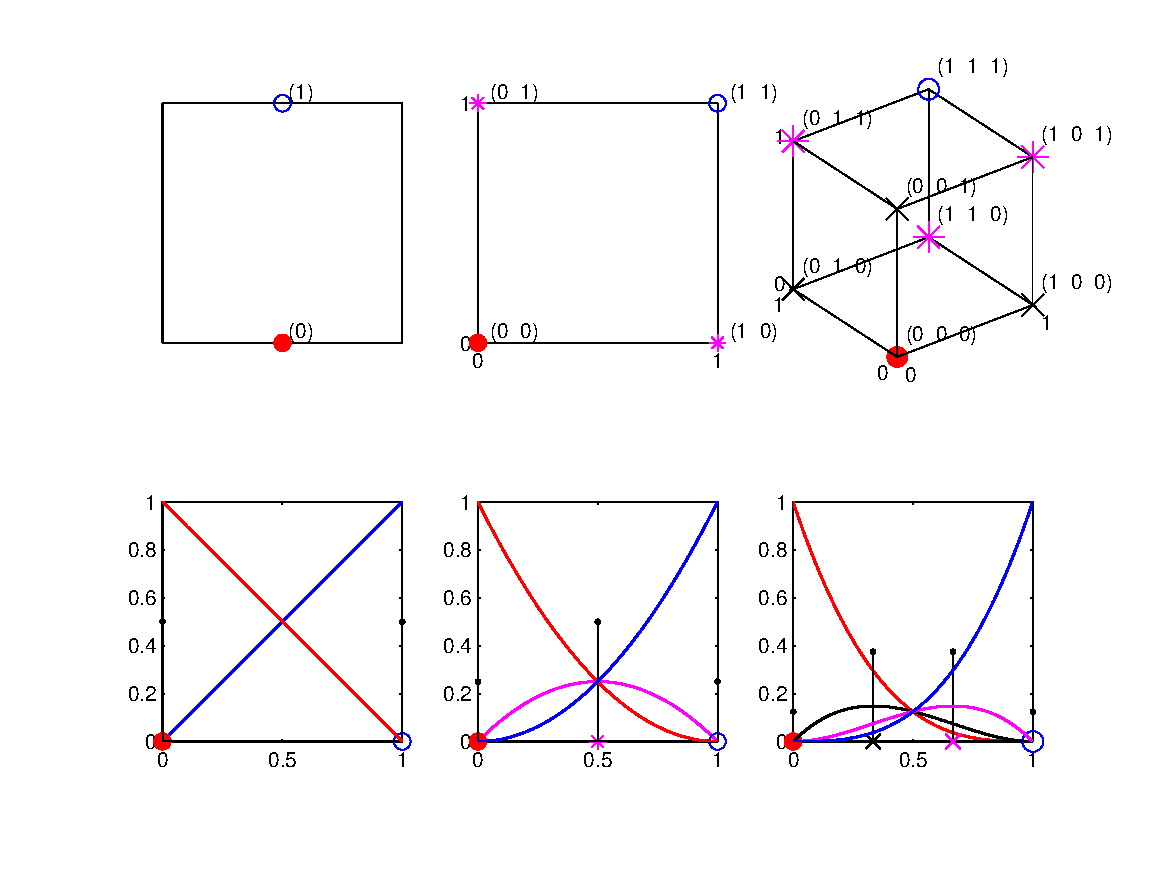
\includegraphics[width=4.5in]{figures/BernoulliSampleLkl}}
\end{figure}

\begin{figure}[ht]
\caption{{\small $100$ realisations of $C_{10}, C_{100}, C_{1000}$ based on samples of size $n$ $=$ $10$, $100$ and $1000$ drawn from the $\bernoulli(\theta^*=0.5)$ RV as per \hyperref[Mf:BernoulliMLEConsistency]{Labwork~\ref*{Mf:BernoulliMLEConsistency}}.  The MLE $\widehat{\theta}_n$ (cyan dot) and the log-likelihood function (magenta curve) for each of the $100$ replications of the experiment for each sample size $n$ are depicted.  The approximate normal-based $95\%$ confidence intervals with blue boundaries are based on the exact $\mathsf{se}_n=\sqrt{\theta^*(1-\theta^*)/n}=\sqrt{1/4}$, while those with red boundaries are based on the estimated $\widehat{\mathsf{se}_n}=\sqrt{\widehat{\theta}_n(1-\widehat{\theta}_n)/n}$.  The fraction of times the true parameter $\theta^*=0.5$ was engulfed by the exact and approximate confidence interval (empirical coverage) over the $100$ replications of the experiment for each of the three sample sizes are given by the numbers after {\tt Cvrg.=} and {\tt $\sim$=}, above each sub-plot, respectively.}\label{F:BernoulliMLEConsistency}}
\begin{center}
\makebox{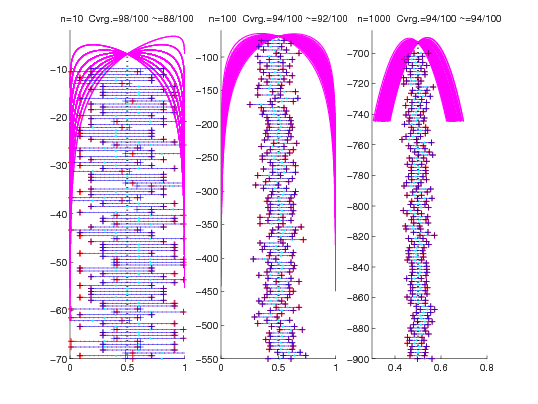
\includegraphics[width=4.50in]{figures/BernoulliMLEConsistency}}
\end{center}
\end{figure}  


%Let us look at some examples of estimation.





\section{Parameter Estimation and Likelihood}\label{S:ParamEstAndLikelihood}

Now that we have been introduced to point and set estimation of the population mean and the population proportion using the notion of convergence in distribution for sequences of RVs as well as concentration inequalities, 
we can begin to appreciate the art of estimation in a more general setting.  
Parameter estimation is the basic problem in statistical inference and machine learning.  
We will formalize the general estimation problem here.  

As we have already seen, when estimating the population mean or population proportion, there are two basic types of estimators.  
In point estimation we are interested in estimating a particular point of interest that is supposed to belong to a set of points.  
In (confidence) set estimation, we are interested in estimating a set with a particular form that has a specified probability of ``trapping'' the particular point of interest from a set of points.  
Here, a point should be interpreted as an element of a collection of elements from some space.

\subsection{Point and Set Estimation -- A General Likelihood Approach}\label{S:PointSetEstimationLikelihood}
{\bf Point estimation} is any statistical methodology that provides one with a ``{\bf single best guess}'' of some specific quantity of interest.  Traditionally, we denote this {\bf quantity of interest as $\theta^*$} and {\bf its point estimate as $\widehat{\theta}$ or $\widehat{\theta}_n$}.  The subscript $n$ in the point estimate $\widehat{\theta}_n$ emphasizes that our estimate is based on $n$ observations or data points from a given statistical experiment to estimate $\theta^*$.  This quantity of interest, which is usually unknown, can be: %, namely $\theta$
%, may be an {\bf integral} $\Iz$ of a real valued function $h(x)$, i.e.~$\theta=\Iz := \int_a^b h(x)\,dx \in \Rz$, or simply a 
\begin{itemize}
\item a {\bf parameter} $\theta^*$ which is an element of the {\bf parameter space} $\BB{\Theta}$, i.e.~$\theta^* \in \BB{\Theta}$ such that $\theta^*$ specifies the ``law'' of the observations (realizations or samples) of the \rv~$(X_1,\ldots,X_n)$ modeled by JPDF or JPMF $f_{X_1,\ldots,X_n}(x_1,\ldots,x_n; \theta^*)$, or
%\item a {\bf distribution function (DF)} $F^* \in \Fz := \text{the set of all DFs}$
%\item a {\bf density function (pdf)} $f \in \{ \text{``not too wiggly Sobolev functions''} \}$, or 
\item a {\bf regression function} $\theta^* \in \BB{\Theta}$, where $\BB{\Theta}$ is a class of regression functions in a regression experiment with model: $Y=\theta^*(X)+\epsilon$, such that $\e(\epsilon)=0$ and $\theta^*$ specifies the ``law'' of pairs of observations $\{(X_i,Y_i)\}_{i=1}^n$, for e.g., fitting parameters in noisy ODE or PDEs from observed data --- one can always do a {\bf prediction} in a regression experiment, i.e.~when you want to estimate $Y_i$ given $X_i$, or
\item a {\bf classifier} $\theta^* \in \BB{\Theta}$, i.e.~a regression experiment with discrete $Y = \theta^*(X)+\epsilon$, for e.g.~training an scrub-nurse robot to assist a human surgeon, or 
\item an {\bf integral} $\theta^* := \int_A h(x)\,dx \in \BB{\Theta}$.  If $\theta^*$ is finite, then $\BB{\Theta} =  \Rz$, for e.g.~$\theta^*$ could be the volume of a high-dimensional irregular polyhedron, a traffic congestion measure on a network of roadways, the expected profit from a new brew of beer, or the probability of an extreme event such as the collapse of a dam in the Southern Alps in the next 150 years.%  For e.g.~see \ref{S:BMC} on Monte Carlo integration.
\end{itemize}
{\bf Set estimation} is any statistical methodology that provides one with a ``{\bf best smallest set}'', such as an interval, rectangle, ellipse, etc.~that contains $\theta^*$ with a high probability $1-\alpha$.

Recall that a statistic is a RV or \rv~$T(X)$ that maps every data point $x$ in the data space $\Xz$ with $T(x)=t$ in its range $\Tz$, i.e.~$T(x):\Xz \to \Tz$ (\hyperref[D:Statistic]{Definition~\ref*{D:Statistic}}).  
Next, we look at a specific class of statistics whose range is the parameter space $\BB{\Theta}$.

\begin{definition}[Point Estimator]\label{D:Estimator}
%{\rm
A {\bf point estimator} $\widehat{\Theta}$ of some {\bf fixed and possibly unknown} $\theta^* \in \BB{\Theta}$ is a statistic that associates each data point $x \in \Xz$ with a {\bf point estimate} $\widehat{\Theta}(x)=\widehat{\theta} \in \BB{\Theta}$,  
\[
\boxed{
 \widehat{\Theta} := \widehat{\Theta}(x)=\widehat{\theta}: \Xz \to \BB{\Theta}
 } \ .
\]
If our data point $x := (x_1,x_2,\ldots,x_n)$ is an $n$-vector or a point in the $n$-dimensional real space, i.e.~$x := (x_1,x_2,\ldots,x_n) \in \Xz_n \subset \Rz^n$, then we emphasize the dimension $n$ in our point estimator $\widehat{\Theta}_n$ of $\theta^* \in \BB{\Theta}$.
\[
\boxed{
\widehat{\Theta}_n :=  \widehat{\Theta}_n(x:=(x_1,x_2,\ldots,x_n))=\widehat{\theta}_n : \Xz_n \to \BB{\Theta}, \quad \Xz_n \subset \Rz^n 
} \ .
\]
The typical situation for us involves point {\bf estimation} of $\theta^* \in \BB{\Theta}$ from 
$(x_1,x_2,\ldots,x_n)$, the {\bf observed data} (realization or sample), based on the {\bf model}
\[
X=(X_1,X_2,\ldots,X_n) \sim f_{X_1,X_2,\ldots,X_n}(x_1,x_2,\ldots,x_n; \theta^*) \enspace .
\]
%}
\end{definition}

\begin{example}[Coin Tossing Experiment ($X_1,\ldots,X_n \overset{IID}{\sim} \bernoulli(\theta^*)$)]\label{EX:CoinTossing}
{\rm
I tossed a coin that has an unknown probability $\theta^*$ of landing Heads independently and identically $10$ times in a row.  Four of my outcomes were Heads and the remaining six were Tails, with the actual sequence of Bernoulli outcomes (Heads $\to 1$ and Tails $\to 0$) being $(1,0,0,0,1,1,0,0,1,0)$.  I would like to estimate the probability $\theta^* \in \BB{\Theta} = [0,1]$ of observing Heads using the natural estimator $\widehat{\Theta}_n((X_1,X_2,\ldots,X_n))$ of $\theta^*$:
\[
\widehat{\Theta}_n((X_1,X_2,\ldots,X_n)) := \widehat{\Theta}_n = \frac{1}{n} \sum_{i=1}^n X_i =: \overline{X}_n
\]
For the coin tossing experiment I just performed ($n=10$ times), the point estimate of the unknown $\theta^*$ is:
\begin{eqnarray}
\widehat{\theta}_{10} = \widehat{\Theta}_{10}((x_1,x_2,\ldots,x_{10})) 
&=&\widehat{\Theta}_{10}((1,0,0,0,1,1,0,0,1,0)) \notag \\
&=& \frac{1+0+0+0+1+1+0+0+1+0}{10}=\frac{4}{10}=0.40 \notag \ .
\end{eqnarray}
}
\end{example}

\subsection{Likelihood}\label{S:Likelihood}
We take a look at {\bf likelihood} --- one of the most fundamental concepts in Statistics.  

\begin{definition}[Likelihood Function]\label{D:LklFn}
{\rm
Suppose $(X_1,X_2,\ldots,X_n)$ is a \rv~with JPDF or JPMF $f_{X_1,X_2,\ldots,X_n}(x_1,x_2,\ldots,x_n; \theta)$ specified by parameter $\theta \in \BB{\Theta}$.  
Let the observed data be $(x_1,x_2,\ldots,x_n)$.  
Then the {\bf likelihood} function given by $L_n(\theta)$ is merely the joint probability of the data, with the exception that we see it as a function of the parameter:
\begin{equation}
\boxed{
L_n(\theta) := L_n(x_1,x_2,\ldots,x_n; \theta) = f_{X_1,X_2,\ldots,X_n}(x_1,x_2,\ldots,x_n; \theta) \enspace .
}
\end{equation}
The {\bf log-likelihood} function is defined by:
\begin{equation}
\boxed{
\ell_n(\theta) := \log(L_n(\theta))
} \enspace
\end{equation}
}
\end{definition}

\begin{example}[Likelihood of the IID $\bernoulli(\theta^*)$ experiment]\label{EX:LklCoinTossing}
{\rm
Consider our IID Bernoulli experiment:
$$
X_1,X_2,\ldots,X_n \overset{IID}{\sim} \bernoulli(\theta^*), \text{ with PDF } f_{X_i}(x_i;\theta)=\theta^{x_i}(1-\theta)^{1-x_i} \BB{1}_{\{0,1\}}(x_i), \, \text{for } i \in \{1,2,\ldots,n\} \enspace .
$$
Let us understand the likelihood function for one observation first.  There are two possibilities for the first observation.  

If we only have one observation and it happens to be $x_1=1$, then our likelihood function is:
$$L_1(\theta)=L_1(x_1;\theta)
= f_{X_1}(x_1;\theta)
=\theta^{1}(1-\theta)^{1-1} \BB{1}_{\{0,1\}}(1)
=\theta (1-\theta)^0 1
=\theta \enspace
$$
If we only have one observation and it happens to be $x_1=0$, then our likelihood function is:
$$L_1(\theta)=L_1(x_1;\theta)
= f_{X_1}(x_1;\theta)
=\theta^{0}(1-\theta)^{1-0} \BB{1}_{\{0,1\}}(0)
=1 (1-\theta)^1 1
=1-\theta \enspace
$$
If we have $n$ observations $(x_1,x_2,\ldots,x_n)$, i.e.~a vertex point of the unit hyper-cube $\{0,1\}^n$ (see top panel of Figure~\ref{F:BernoulliSampleLkl} when $n \in \{1,2,3\}$), then our likelihood function (see bottom panel of Figure~\ref{F:BernoulliSampleLkl}) is obtained by multiplying the densities due to our IID assumption:
\begin{eqnarray}\label{E:LklBernoulli}
L_n(\theta) &:=& L_n(x_1,x_2,\ldots,x_n; \theta)  = f_{X_1,X_2,\ldots,X_n}(x_1,x_2,\ldots,x_n ; \theta) \notag \\
&=& f_{X_1}(x_1 ; \theta) f_{X_2}(x_2 ; \theta) \cdots f_{X_n}(x_n ; \theta) := \prod_{i=1}^n f_{X_i}(x_i ; \theta) \notag \\
&=& \theta^{\sum_{i=1}^n x_i} (1-\theta)^ {n-\sum_{i=1}^n x_i} %:= \theta^{t_n} (1-\theta)^{n-t_n} \notag 
\end{eqnarray}
%In the last step, we have formally defined the following statistic of the data: 
%$$T_n(X_1,X_2,\ldots,X_n)=\sum_{i=1}^n X_i :  \Xz_n \rightarrow \Tz_n$$ with the corresponding realisation $t_n := T_n(x_1,x_2,\ldots,x_n)=\sum_{i=1}^n x_i \in \Tz_n$. 
}
\end{example}

\begin{figure}[htbp]
\caption{Data Spaces $\Xz_1=\{0,1\}$, $\Xz_2=\{0,1\}^2$ and $\Xz_3=\{0,1\}^3$ for one, two and three IID Bernoulli trials, respectively and the corresponding likelihood functions.\label{F:BernoulliSampleLkl}}
\centering   \makebox{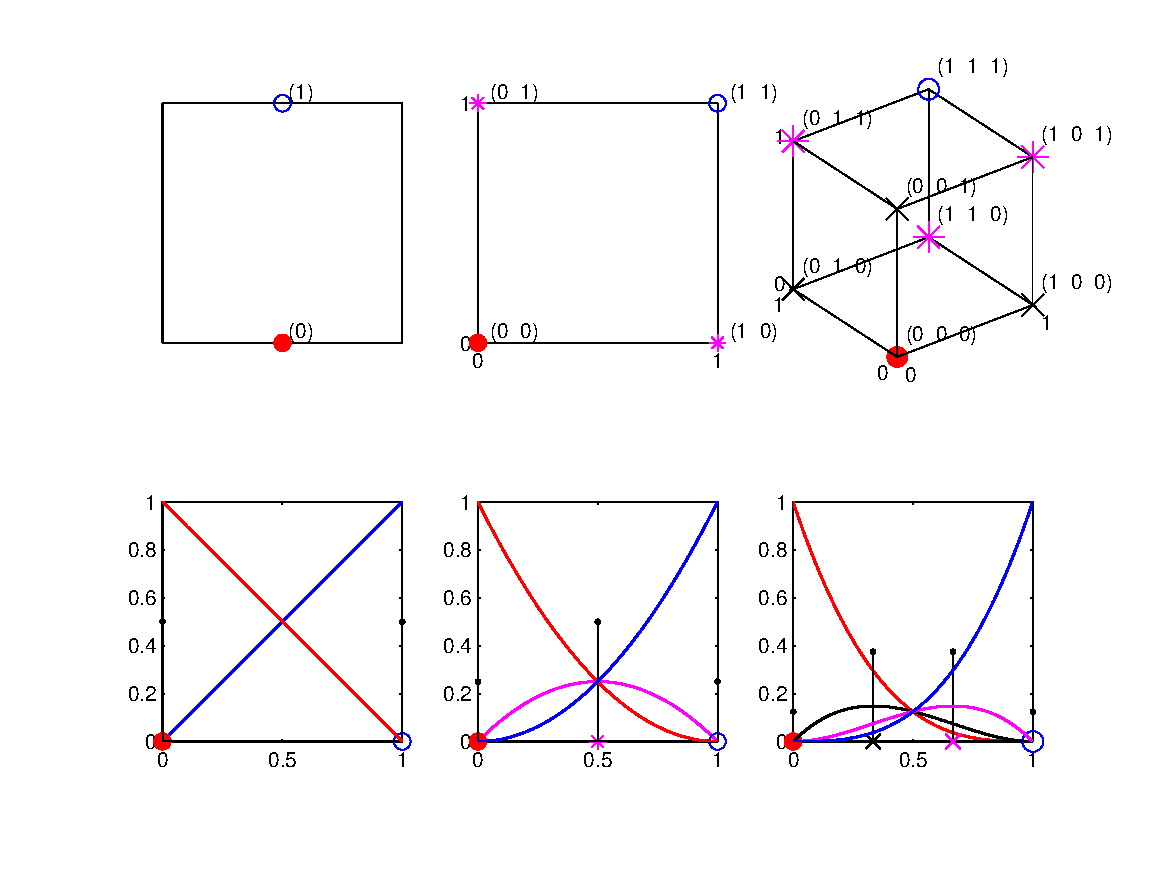
\includegraphics[width=5.0in]{figures/BernoulliSampleLkl}}
\end{figure}


\begin{definition}[Maximum Likelihood Estimator (MLE)]\label{D:MLE}
{\rm
Let the model for the data be
$$(X_1,\ldots,X_n) \sim f_{X_1,X_2,\ldots,X_n}(x_1,\ldots,x_n;\theta^*) \enspace .$$ 
Then the maximum likelihood estimator (MLE) $\widehat{\Theta}_n$ of the fixed and possibly unknown parameter $\theta^* \in \BB{\Theta}$ is the value of $\theta$ that maximizes the likelihood function:
\[
\boxed{
\widehat{\Theta}_n := \widehat{\Theta}_n(X_1,X_2,\ldots,X_n) :=  \argmax_{\theta \in \BB{\Theta}} L_n(\theta) \enspace ,
}
\]
Equivalently, MLE is the value of $\theta$ that maximizes the log-likelihood function (since $\log=\log_e=\ln$ is a monotone increasing function):
\[
\boxed{
\widehat{\Theta}_n := \argmax_{\theta \in \BB{\Theta}} \ell_n(\theta) \enspace ,
}
\]
}
\end{definition}

\subsubsection*{Useful Properties of the Maximum Likelihood Estimator}
\be
\item The ML Estimator is {\em asymptotically consistent} (gives the ``true'' $\theta^*$ as sample size $n \to \infty$):
\[
\boxed{\widehat{\Theta}_n \rightsquigarrow \pointmass(\theta^*)}
\]
\item The ML Estimator is asymptotically normal (has a normal distribution concentrating on $\theta^*$ as $n \to \infty$):
\[
\boxed{\widehat{\Theta}_n \rightsquigarrow \normal(\theta^*,(\widehat{\mathsf{se}}_n)^2)}
\]
or equivalently:
\[
\boxed{(\widehat{\Theta}_n - \theta^*) / \widehat{\mathsf{se}}_n \rightsquigarrow \normal(0,1)}
\]
where $\widehat{\mathsf{se}}_n$ is the {\bf estimated standard error}, i.e.~the standard deviation of $\widehat{\Theta}_n$, and it is given by the square-root of the inverse negative curvature of $\ell_n(\theta)$ at $\widehat{\theta}_n$:
\[
\boxed{
\widehat{\mathsf{se}}_n = \sqrt{\left( \left[ -\frac{d^2 \ell_n(\theta)}{d \theta^2}\right]_{\theta=\widehat{\theta}_n}\right)^{-1}}
}
\]
\item Because of the previous two properties, the $1-\alpha$ confidence interval is:
\[
\boxed{
\widehat{\Theta}_n \pm z_{\alpha/2} \widehat{\mathsf{se}}_n 
}
\]
%\item The ML Estimator is {\bf equivariant}, i.e.~$\widehat{\psi}_n=g(\widehat{\theta}_n)$ is the ML Estimate of $\psi^*=g(\theta^*)$, for some smooth function $g(\theta)=\psi: \BB{\Theta} \to \BB{\Psi}$.  
\ee

MLE is a general methodology for parameter estimation in an essentially arbitrary parameter space $\BB{\Theta}$ that is defining or indexing the laws in a parametric family of models, although we are only seeing it in action when $\BB{\Theta} \subset \Rz$ for simplest parametric family of models involving IID product experiments here.  
When $\BB{\Theta} \subset \Rz^d$ with $2 \leq d < \infty$ then MLE $\widehat{\Theta}_n \rightsquigarrow \pointmass(\theta^*)$, where $\theta^*=(\theta^*_1,\theta^*_2,\ldots,\theta^*_d)^{T}$ is a column vector in $\BB{\Theta} \subset \Rz^d$ 
and $\widehat{\Theta}_n \rightsquigarrow \normal\left(\theta^*,\widehat{\Sigma(\mathsf{se})}_n\right)$, a multivariate Normal distribution with mean vector $\theta^*$ and variance-covariance matrix of standard errors given by the {\em Hessian} (a $d \times d$ matrix of mixed partial derivatives) of $\ell_n(\theta_1,\theta_2,\ldots,\theta_d)$.  The ideas in the cased of dimension $d=1$ naturally generalize to an arbitrary, but finite, dimension $d$.
 
\begin{rem}
In order to use MLE for parameter estimation we need to ensure that the following two conditions hold:
\be
\item The {\em support} of the data, i.e.~the set of possible values of $(X_1,X_2,\ldots,X_n)$ must not depend on $\theta$ for every $\theta \in \BB{\Theta}$ --- of course the probabilities do depend on $\theta$ in an {\em identifiable} manner, i.e.~for every $\theta$ and $\vartheta$ in $\BB{\Theta}$, if $\theta \neq \vartheta$ then $f_{X_1,X_2,\ldots,X_n}(x_1,x_2,\ldots,x_n;\theta) \neq f_{X_1,\ldots,X_n}(x_1,x_2,\ldots,x_n;\vartheta)$ at least for some $(x_1,x_2,\ldots,x_n) \in \Xz$.
\item If the parameter space $\BB{\Theta}$ is bounded then $\theta^*$ must not belong to the boundaries of $\BB{\Theta}$.
\ee
\end{rem}

\subsubsection*{Maximum Likelihood Estimation Method in Six Easy Steps}
{\bf Background:} We have observed data:
\[
(x_1,x_2,\ldots,x_n)
\]
which is modeled as a sample or realization from the random vector:
\[
(X_1,X_2,\ldots,X_n) \sim f_{X_1,X_2,\ldots,X_n}(x_1,x_2,\ldots,x_n; \theta^*), \quad \theta^* \in \BB{\Theta} \enspace .
\]
{\bf Objective:} We want to obtain an estimator $\widehat{\Theta}_n$ that will give:
\be
\item the point estimate $\widehat{\theta}_n$ of the ``true'' parameter $\theta^*$ and
\item the $(1-\alpha)$ confidence interval for $\theta^*$.
\ee
{\bf Steps of MLE:} 
\begin{itemize}
\item{{\sf Step 1}:} Find the expression for the log likelihood function:
\[
\ell_n(\theta) = \log(L_n(\theta)) = \log\left( f_{X_1,X_2,\ldots,X_n}(x_1,x_2,\ldots,x_n; \theta) \right) \enspace .
\]
Note that if the model assumes that $(X_1,X_2,\ldots,X_n)$ is jointly independent, i.e.~we have an independent and identically distributed (IID) experiment, then $\ell_n(\theta)$ simplifies further as follows:
\[
\ell_n(\theta) = \log(L_n(\theta)) = \log\left( f_{X_1,X_2,\ldots,X_n}(x_1,x_2,\ldots,x_n; \theta) \right) = \log \left(\prod_{i=1}^n f_{X_i}(x_i;\theta) \right) %= \sum_{i=1}^n \log\left(f_{X_i}(x_i;\theta)\right) 
\enspace .
\]

\item{{\sf Step 2}:} Obtain the derivative of $\ell_n(\theta)$ with respect to $\theta$:
\[
\frac{d}{d \theta}\left(\ell_n(\theta)\right) \enspace .
\]
\item{{\sf Step 3}:} Set the derivative equal to zero, solve for $\theta$ and let $\widehat{\theta}_n$ equal to this solution. 
\item{{\sf Step 4}:} Check if this solution is indeed a maximum of $\ell_n(\theta)$ by checking  if:
\[
\frac{d^2}{d \theta^2}\left(\ell_n(\theta)\right) < 0 \enspace .
\]
\item{{\sf Step 5}:} If $\frac{d^2}{d \theta^2}\left(\ell_n(\theta)\right) < 0$ then you have found the maximum likelihood estimate $\widehat{\theta}_n$.
\item{{\sf Step 6}:} If you also want the $(1-\alpha)$ confidence interval then get it from
\[
\widehat{\theta}_n \pm z_{\alpha/2} \widehat{\mathsf{se}}_n \quad \text{, where } \quad \widehat{\mathsf{se}}_n = \sqrt{\left( \left[ -\frac{d^2 \ell_n(\theta)}{d \theta^2}\right]_{\theta=\widehat{\theta}_n}\right)^{-1}} \enspace .
\]
\end{itemize}

Let us apply this method in some examples.


{
\begin{example}[Maximum likelihood estimation for IID $\exponential(\lambda^*)$ trials]\label{Eg:ExponentialMLE}
Find (or derive) the maximum likelihood estimate $\widehat{\lambda}_n$ and the $(1-\alpha)$ confidence interval of the fixed and possibly unknown parameter $\lambda^*$ for the IID experiment:
$$X_1,\ldots,X_n \overset{IID}{\sim} \exponential(\lambda^*), \qquad \lambda^* \in \BB{\Lambda} = (0,\infty) \enspace .$$
Note that $\BB{\Lambda}$ is the parameter space.

We first obtain the log-likelihood function $\ell_n(\theta)$ given data $(x_1,x_2,\ldots,x_n)$.
\begin{flalign*}
\ell_n(\lambda) 
& := \log(L(x_1,x_2,\ldots,x_n;\lambda))  = \log \left( \prod_{i=1}^n f_{X_i}(x_i;\lambda) \right) = \log \left( \prod_{i=1}^n \lambda e^{-\lambda x_i}  \right)\\
& = \log \left( \lambda e^{-\lambda x_1} \cdot \lambda e^{-\lambda x_2}  \cdots \lambda e^{-\lambda x_n}  \right) = \log \left( \lambda^n e^{-\lambda \sum_{i=1}^n x_i}  \right) =\log \left( \lambda^n \right) + \log \left( e^{-\lambda \sum_{i=1}^n x_i}  \right) \\
&= \boxed{\log \left( \lambda^n \right) -\lambda \sum_{i=1}^n x_i}
\end{flalign*}

Now, let us take the derivative with respect to $\lambda$,
\begin{flalign*}
\frac{d}{d \lambda} \left( \ell_n(\lambda) \right) 
& :=  \frac{d}{d \lambda} \left( 
\log \left( \lambda^n \right) -\lambda \sum_{i=1}^n x_i
\right) = \frac{d}{d \lambda} \left( 
\log \left( \lambda^n \right) \right) -  \frac{d}{d \lambda} \left( \lambda \sum_{i=1}^n x_i \right)  = \frac{1}{\lambda^n}  \frac{d}{d \lambda} \left( \lambda^n \right) - \sum_{i=1}^n x_i \\
&= \frac{1}{\lambda^n}  n \lambda^{n-1}  - \sum_{i=1}^n x_i = \boxed{\frac{n}{\lambda} - \sum_{i=1}^n x_i } \enspace .
\end{flalign*}
Next, we set the derivative to $0$, solve for $\lambda$, and let the solution equal to the ML estimate $\widehat{\lambda}_n$.
\begin{flalign*}
0 = \frac{d}{d \lambda} \left( \ell_n(\lambda) \right) 
& \iff 0 = \frac{n}{\lambda} - \sum_{i=1}^n x_i \iff \sum_{i=1}^n x_i = \frac{n}{\lambda} \iff \lambda = \frac{n}{\sum_{i=1}^n x_i} \quad \text{ and let } \boxed{\widehat{\lambda}_n = \frac{1}{\overline{x}_n}} \enspace .
\end{flalign*}
Next, we find the second derivative and check if it is negative.
\begin{flalign*}
\frac{d^2}{d \lambda^2} \left( \ell_n(\lambda) \right) 
&= \frac{d}{d \lambda} \left( \frac{d}{d \lambda} \left( \ell_n(\lambda) \right) \right) = \frac{d}{d \lambda} \left( \frac{n}{\lambda} - \sum_{i=1}^n x_i \right) = \boxed{-n\lambda^{-2}} \enspace .
\end{flalign*}
Since $\lambda>0$ and $n \in \Nz$, $\boxed{-n\lambda^{-2}=-n/\lambda^2 < 0}$, so we have found the maximum likelihood estimate:
\[
\boxed{\widehat{\lambda}_n = \frac{1}{\overline{x}_n} } \enspace .
\]
Now, let us find the estimated standard error:
\begin{align*}
\boxed{\widehat{\mathsf{se}}_n} 
&= \sqrt{\left( \left[ -\frac{d^2 \ell_n(\lambda)}{d \lambda^2}\right]_{\lambda=\widehat{\lambda}_n}\right)^{-1}} 
= \sqrt{\left( \left[ - \left( -\frac{n}{\lambda^2}\right) \right]_{\lambda=\widehat{\lambda}_n}\right)^{-1}} = \sqrt{\left( \frac{n}{\widehat{\lambda}_n^2}\right)^{-1}}=\sqrt{\frac{\widehat{\lambda}_n^2}{n}}=\frac{\widehat{\lambda}_n}{\sqrt{n}}\\
&=\boxed{\frac{1}{\ol{x}_n\sqrt{n}}}
\enspace .
\end{align*}
And finally, the $(1-\alpha)$ confidence interval is
\[
\widehat{\lambda}_n \pm z_{\alpha/2} \widehat{\mathsf{se}}_n 
= \boxed{\frac{1}{\overline{x}_n} \pm z_{\alpha/2} \frac{1}{\ol{x}_n\sqrt{n}}} \enspace . 
\]
\end{example}
}

Since we have worked ``hard'' to get the maximum likelihood estimate for a general IID model $X_1,X_2,\ldots,X_n \overset{IID}{\sim} \exponential(\lambda^*)$.  Let us kill two birds with the same stone by applying it to two datasets:
\be
\item Orbiter waiting times and
\item Time between measurable earthquakes in New Zealand over a few months.
\ee
Therefore, the ML estimate $\widehat{\lambda}_n$ of the unknown rate parameter $\lambda^* \in \BB{\Lambda}$ on the basis of $n$ IID observations $x_1,x_2,\ldots,x_n \overset{IID}{\sim} \exponential(\lambda^*)$ is $1/\overline{x}_n$ and the ML estimator $\widehat{\Lambda}_n=1/\overline{X}_n$.  

\begin{example}[Orbiter Waiting Times]\label{EgOrbiterMLE}
Let us apply this ML estimator of the rate parameter for the supposedly exponentially distributed waiting times at the on-campus Orbiter bus-stop.

Joshua Fenemore and Yiran Wang collected data on waiting times between buses at an Orbiter bus-stop close to campus.  
They collected a sample of size $n=132$ with sample mean $\overline{x}_{132}=9.0758$.
\begin{VrbM}
% Joshu Fenemore’s Data from 2007 on Waiting Times at Orbiter Bust Stop by Balgay Street
%The raw data -- the waiting times to nearest minute between Orbiter buses
>> orbiterTimes=[8 3 7 18 18 3 7 9 9 25 0 0 25 6 10 0 10 8 16 9 1 5 16 6 4 1 3 21 0 28 3 8 ...
 6 6 11 8 10 15 0 8 7 11 10 9 12 13 8 10 11 8 7 11 5 9 11 14 13 5 8 9 12 10 13 6 11 13 ...
 0 0 11 1 9 5 14 16 2 10 21 1 14 2 10 24 6 1 14 14 0 14 4 11 15 0 10 2 13 2 22 ...
 10 5 6 13 1 13 10 11 4 7 9 12 8 16 15 14 5 10 12 9 8 0 5 13 13 6 8 4 13 15 7 11 6 23 1];
>> mean(orbiterTimes)
ans =
    9.0758
\end{VrbM}

From our work in Example~\ref{Eg:ExponentialMLE} we can now easily obtain the maximum likelihood estimate of $\lambda^*$ and the $95\%$ confidence interval for it, under the assumption that the waiting times $X_1,\ldots,X_{132}$ are IID $\exponential(\lambda^*)$ RVs as follows: 
$$\widehat{\lambda}_{132}=1/\overline{x}_{132}=1/9.0758=0.1102 \quad 
(0.1102 \pm 1.96 \times 0.1102/\sqrt{132}) = (0.0914,0.1290) \enspace ,$$ 
and thus the estimated mean waiting time is 
$$1/\widehat{\lambda}_{132}=9.0763 \text{ minutes} .$$  
The estimated mean waiting time for a bus to arrive is well within the $10$ minutes promised by the Orbiter bus company.  
This data and its maximum likelihood analysis is presented visually in Figure~\ref{F:ExponentialMLEOrbiter}.
 
The following script was used to generate the \hyperref[F:ExponentialMLE]{Figure \ref*{F:ExponentialMLEOrbiter}}:
\begin{figure}[htpb]
\caption{Plot of $\log(L(\lambda))$ as a function of the parameter $\lambda$  and the MLE $\widehat{\lambda}_{132}$ of $0.1102$ for Fenemore-Wang Orbiter Waiting Times Experiment from STAT 218 S2 2007.  The density or PDF and the DF at the MLE of $0.1102$ are compared with a histogram and the empirical DF.\label{F:ExponentialMLEOrbiter}}
\centering   \makebox{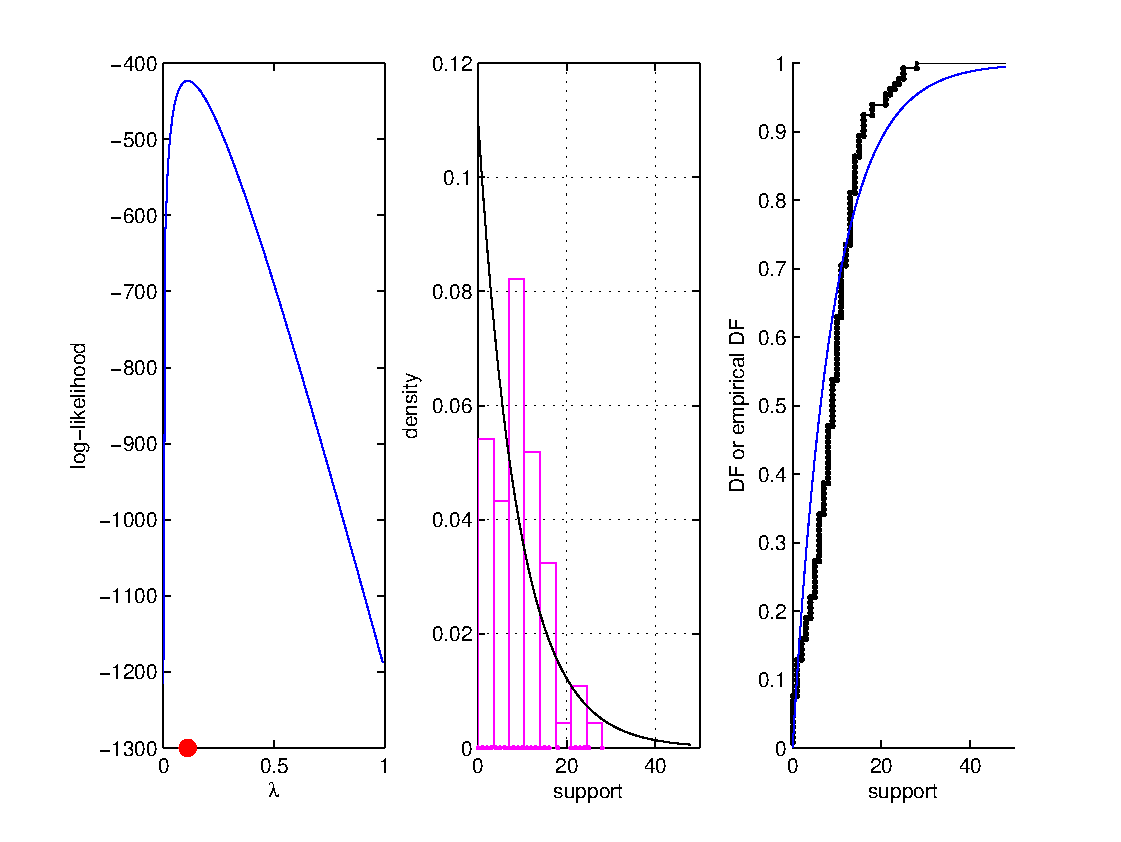
\includegraphics[width=4.5in]{figures/ExponentialMLEOrbiter}}
\end{figure}
Notice how the exponential PDF $f(x;\widehat{\lambda}_{132}=0.1102)$ and the DF $F(x;\widehat{\lambda}_{132}=0.1102)$ based on the MLE fits with the histogram and the empirical DF, respectively.  
%This is an indication of the inadequacy of our parametric model.  Partly this discrepancy is due to the resolution of the the measurements being confined to whole minutes.  We can overcome this problem by fitting a minute-discretized PMF from the $\exponential(\lambda)$ PDF.  

\begin{figure}[htpb]
\caption{Comparing the $\exponential(\widehat{\lambda}_{6128}= 28.6694)$ PDF and DF with a histogram and empirical DF of the times (in units of days) between earth quakes in  NZ.  The epicenters of $6128$ earth quakes are shown in left panel.\label{F:NZSIEarthQuakesExponentialMLE}}
\centering   \makebox{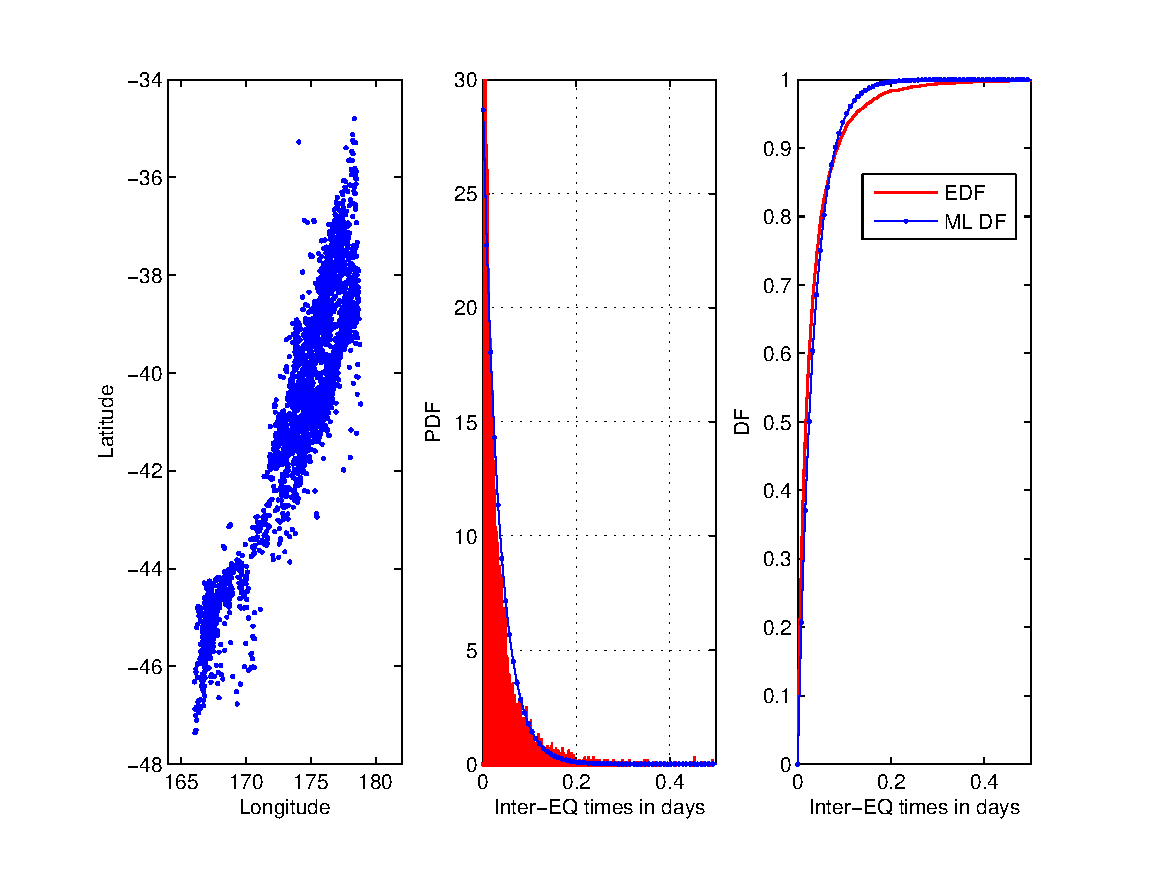
\includegraphics[width=4.5in]{figures/NZSIEarthQuakesExponentialMLE}}
\end{figure}
\end{example}

\begin{example}[Waiting Times between Earth Quakes in NZ]\label{LW:NZSIEarthQuakesExponentialMLE}  
Once again from our work in Example~\ref{Eg:ExponentialMLE} we can now easily obtain the maximum likelihood estimate of $\lambda^*$ and the $95\%$ confidence interval for it, under the assumption that the waiting times (in days) between the $6128$ measurable earth-quakes in NZ from 18-Jan-2008 02:23:44 to 18-Aug-2008 19:29:29 are IID $\exponential(\lambda^*)$ RVs as follows: 
$$\widehat{\lambda}_{6128}=1/\overline{x}_{6128}=1/0.0349=28.6694 \quad 
(28.6694 \pm 1.96 \times 28.6694/\sqrt{6128}) = (27.95,29.39) \enspace ,$$ 
and thus the estimated mean time in days and minutes between earth quakes (somewhere in NZ over the first 8 months in 2008), as processed in Labwork~\ref{LW:NZSIEarthQuakesExponentialMLE}, is 
$$1/\widehat{\lambda}_{6128}=\overline{x}_{6128}=0.0349 \text{ days } \quad = \quad 0.0349*24*60=50.2560  \text{ minutes} \enspace .$$  
This data and its maximum likelihood analysis is presented visually in Figure~\ref{F:NZSIEarthQuakesExponentialMLE}.  The PDF and DF corresponding to the $\widehat{\lambda}_{6128}$ (blue curves in Figure~\ref{F:NZSIEarthQuakesExponentialMLE}) are the best fitting PDF and DF from the parametric family of PDFs in $\{\lambda e^{-\lambda x}: \lambda \in (0,\infty) \}$ and DFs in $\{1- e^{-\lambda x}: \lambda \in (0,\infty) \}$ to the density histogram and the empirical distribution function given by the data, respectively.  Clearly, there is room for improving beyond the model of IID $\exponential(\lambda)$ RVs, but the fit with just one real-valued parameter is not too bad either.  Finally, with the best fitting PDF $28.6694 e^{-28.6694 x}$ we can get probabilities of events and answer questions like: ``what is the probability that there will be three earth quakes somewhere in NZ within the next hour?'', etc.
\end{example}

\begin{labwork}[Inter Earth Quake Time Processing]\label{LW:NZSIEarthQuakesExponentialMLE}
To process the data to get the times between earth quakes, we can compute as in the following script:\VrbMf[label=NZSIEarthQuakesExponentialMLE.m]{scripts/NZSIEarthQuakesExponentialMLE.m}
We first load the data in the text file {\tt earthquakes.csv} into a matrix {\tt EQ}.  Using the {\tt datenum} function in {\sc Matlab} we transform the time stamps into a number starting at zero.  These transformed time stamps are in units of days.  Then we find the times between consecutive events and estimate a histogram.  We finally compute the ML estimate of $\lambda^*$ and super-impose the PDF of the $\exponential(\widehat{\lambda}_{6128}= 28.6694)$ upon the histogram.
\begin{VrbM}
>> NZSIEarthQuakesExponentialMLE
ans =        6128          13

Earth Quakes in NZ between
18-Jan-2008 02:23:44 and18-Aug-2008 19:29:29

SampleMean =    0.0349
MLELambdaHat =   28.6694
\end{VrbM}
Thus, the average time between earth quakes is $0.0349*24*60=50.2560$ minutes.
\end{labwork}

\begin{example}[ML Estimation for the IID $\bernoulli(\theta^*)$ experiment]\label{EX:MLECoinTossing}
Let us do maximum likelihood estimation for the coin-tossing experiment of Example~\ref{EX:CoinTossing} with likelihood derived in Example~\ref{EX:LklCoinTossing} to obtain the maximum likelihood estimate $\widehat{\theta}_n$ of the unknown parameter $\theta^* \in \BB{\Theta} = [0,1]$ and the $(1-\alpha)$ confidence interval for it.

From Equation~\eqref{E:LklBernoulli} the log likelihood function is
\begin{eqnarray}
\ell_n(\theta) = \log(L_n(\theta)) 
= \log \left( \theta^{\sum_{i=1}^n x_i} (1-\theta)^ {n-\sum_{i=1}^n x_i} \right) 
= \boxed{\left({\sum_{i=1}^n x_i}\right) \log(\theta) + \left(n-{\sum_{i=1}^n x_i}\right) \log(1-\theta)} \notag \enspace ,
\end{eqnarray}
Next, we take the derivative with respect to the parameter $\theta$:
\begin{eqnarray}
\frac{d}{d \theta} \left(\ell_n(\theta)\right) 
&=& \frac{d}{d \theta}  \left( \left({\sum_{i=1}^n x_i}\right) \log(\theta) \right) + \frac{d}{d \theta} \left(  \left( n-{\sum_{i=1}^n x_i} \right) \log(1-\theta) \right) \notag = \boxed{\frac{{\sum_{i=1}^n x_i}}{\theta} - \frac{n-{\sum_{i=1}^n x_i}}{1-\theta}} \notag \enspace .
\end{eqnarray}
Now, set $\frac{d}{d \theta} \log(L_n(\theta))=0$, solve for $\theta$ and set the solution equal to $\widehat{\theta}_n$: 
\begin{align*}
\frac{d}{d \theta} \left( \ell_n(\theta) \right) = 0 
&\iff  \frac{{\sum_{i=1}^n x_i}}{\theta} = \frac{n-{\sum_{i=1}^n x_i}}{1-\theta} \iff
\frac{1-\theta}{\theta} = \frac{n-{\sum_{i=1}^n x_i}}{{\sum_{i=1}^n x_i}} \\
&\iff
\frac{1}{\theta}-1 = \frac{n}{{\sum_{i=1}^n x_i}}-1 \quad \text{ let } \boxed{\widehat{\theta}_n = \frac{{\sum_{i=1}^n x_i}}{n}}
\end{align*}
Next, we find the second derivative and check if it is negative.
\begin{align*}
\frac{d^2}{d \theta^2} (\ell_n(\theta)) 
&= \frac{d}{d \theta} \left( \frac{{\sum_{i=1}^n x_i}}{\theta} - \frac{n-{\sum_{i=1}^n x_i}}{1-\theta} \right) 
= \boxed{-\frac{{\sum_{i=1}^n x_i}}{\theta^2} - \frac{n-{\sum_{i=1}^n x_i}}{(1-\theta)^2}} 
\end{align*}

Since each term in the numerator and the denominator of the two fractions in the above box are non-negative, $\frac{d^2}{d \theta^2} (\ell_n(\theta))< 0$ and therefore we have found the maximum likelihood estimate
\[
\widehat{\theta}_n  = \frac{1}{n} \sum_{i=1}^n x_i = \overline{x}_n
\]
We already knew this to be a point estimate for $E(X_i)=\theta^*$ from LLN and CLT.  But now we know that MLE also agrees.
Now, let us find the estimated standard error:
\begin{align*}
\boxed{\widehat{\mathsf{se}}_n} 
&= \sqrt{\left( \left[ -\frac{d^2 \ell_n(\theta)}{d \theta^2}\right]_{\theta=\widehat{\theta}_n}\right)^{-1}} 
= \sqrt{\left( \left[ - \left( -\frac{{\sum_{i=1}^n x_i}}{\theta^2} - \frac{n-{\sum_{i=1}^n x_i}}{(1-\theta)^2}\right) \right]_{\theta=\widehat{\theta}_n}\right)^{-1}} \\
&= \sqrt{\left( \frac{{\sum_{i=1}^n x_i}}{\widehat{\theta}_n^2} + \frac{n-{\sum_{i=1}^n x_i}}{(1-\widehat{\theta}_n)^2} \right)^{-1}}
= \sqrt{\left( \frac{n\ol{x}_n}{\ol{x}_n^2} + \frac{n-n\ol{x}_n}{(1-\ol{x}_n)^2} \right)^{-1}}
= \sqrt{\left( \frac{n}{\ol{x}_n} + \frac{n}{(1-\ol{x}_n)} \right)^{-1}}\\
&= \sqrt{\left( \frac{n(1-\ol{x}_n)+n\ol{x}_n}{\ol{x}_n(1-\ol{x}_n)} \right)^{-1}}
= \sqrt{\frac{\ol{x}_n(1-\ol{x}_n)}{n((1-\ol{x}_n)+\ol{x}_n}}
= \boxed{\sqrt{\frac{\ol{x}_n(1-\ol{x}_n)}{n}}} \enspace .\\
\enspace .
\end{align*}
And finally, the $(1-\alpha)$ confidence interval is
\[
\widehat{\theta}_n \pm z_{\alpha/2} \widehat{\mathsf{se}}_n 
= \boxed{\overline{x}_n \pm z_{\alpha/2} \sqrt{\frac{\ol{x}_n(1-\ol{x}_n)}{n}}} \enspace . 
\]

For the coin tossing experiment that was performed ($n=10$ times) in Example~\ref{EX:CoinTossing}, the maximum likelihood estimate of $\theta^*$ and the $95\%$ confidence interval for it, under the model that the tosses are IID $\bernoulli(\theta^*)$ RVs, are as follows:
\[
\widehat{\theta}_{10} 
= \ol{x}_{10} =\frac{4}{10}=0.40
\quad \text{and} \quad \left(0.4 \pm 1.96 \times \sqrt{\frac{0.4 \times 0.6}{10}}\right) =  (0.0964, 0.7036) \enspace .
\]
See Figures~\ref{F:BernoulliMLE} and \ref{F:BernoulliMLEConsistency} to completely understand parameter estimation for IID Bernoulli experiments.
% (not just coin toss, but for any event of interest!) through the pictures.
\end{example}

\begin{figure}[htpb]
\caption{Plots of the log likelihood $\ell_n(\theta)=\log(L(1,0,0,0,1,1,0,0,1,0;\theta))$ as a function of the parameter $\theta$ over the parameter space $\BB{\Theta}=[0,1]$ and the MLE $\widehat{\theta}_{10}$ of $0.4$ for the coin-tossing experiment shown in standard scale (left panel) and log scale for $x$-axis (right panel).\label{F:BernoulliMLE}}
\centering   \makebox{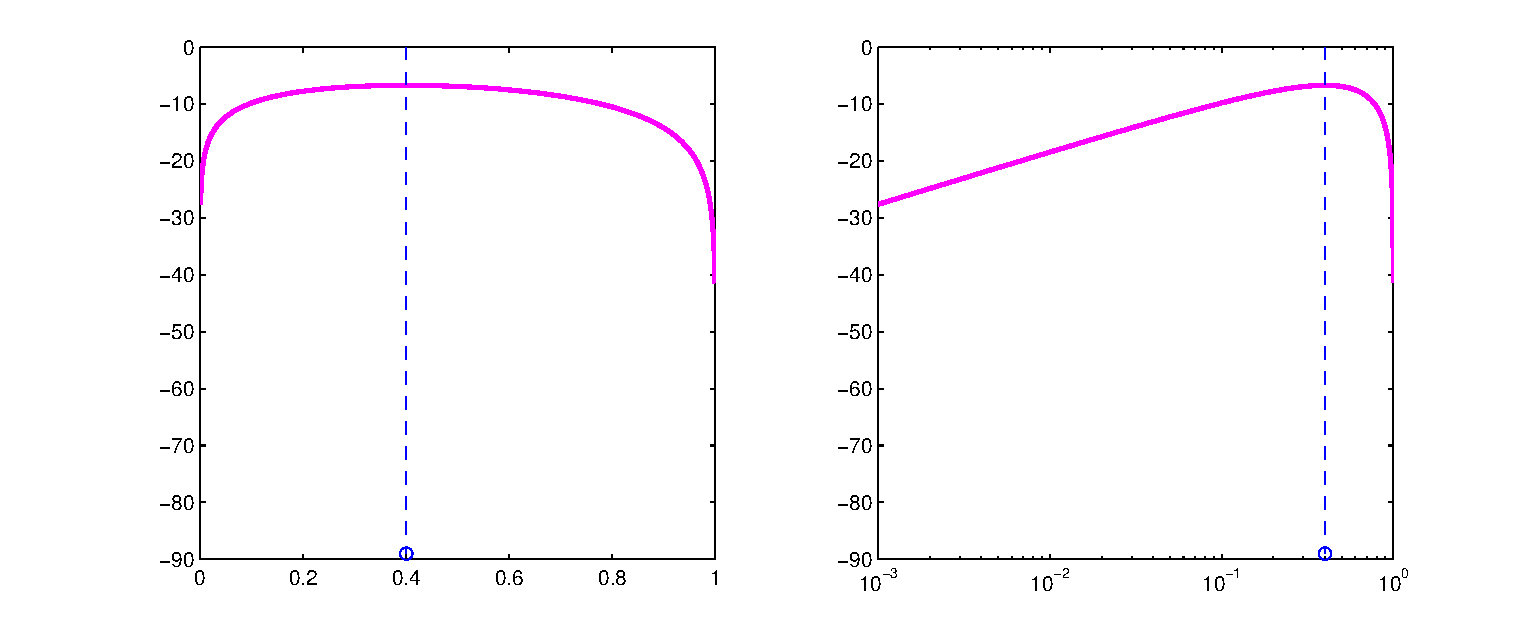
\includegraphics[width=5.5in]{figures/BernoulliMLE}}
\end{figure}


\begin{figure}[htbp]
\caption{{\small $100$ realizations of $95\%$ confidence intervals based on samples of size $n$ $=$ $10$, $100$ and $1000$ simulated from IID $\bernoulli(\theta^*=0.5)$ RVs.  %as per \hyperref[Mf:BernoulliMLEConsistency]{Labwork~\ref*{Mf:BernoulliMLEConsistency}}.  
The MLE $\widehat{\theta}_n$ (cyan dot) and the log-likelihood function (magenta curve) for each of the $100$ replications of the experiment for each sample size $n$ are depicted.  
The approximate normal-based $95\%$ confidence intervals with blue boundaries are based on the exact $\mathsf{se}_n=\sqrt{\theta^*(1-\theta^*)/n}=\sqrt{1/4}$, while those with red boundaries are based on the estimated $\widehat{\mathsf{se}_n}=\sqrt{\widehat{\theta}_n(1-\widehat{\theta}_n)/n} = \sqrt{\frac{\ol{x}_n(1-\ol{x}_n)}{n}}$.  
The fraction of times the true parameter $\theta^*=0.5$ was contained by the exact and approximate confidence interval (known as {\em empirical coverage}) over the $100$ replications of the simulation experiment for each of the three sample sizes are given by the numbers after {\tt Cvrg.=} and {\tt $\sim$=}, above each sub-plot, respectively.}\label{F:BernoulliMLEConsistency}}
\begin{center}
\makebox{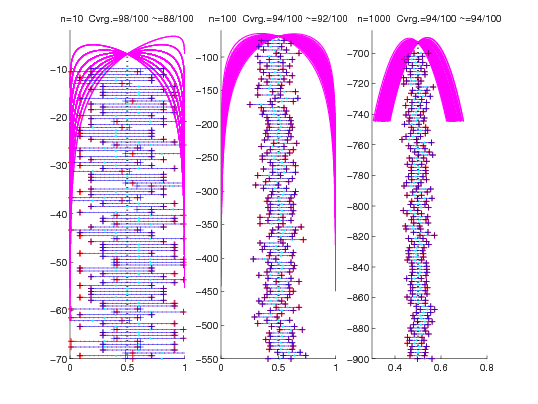
\includegraphics[width=6.00in]{figures/BernoulliMLEConsistency}}
\end{center}
\end{figure}  

\clearpage

%\iftoggle{PlaceTutsHere}{%
%\subsection{Tutorial Exercises}
%\input{Tutorials/Tut_Lkl_preps.tex}
%~\\
%\input{Tutorials/Tut_Lkl_inTut.tex}
%}{%
%  % don't do anything otherwise
%}

\begin{Exercise}[title={Likelihoods of tiny $\bernoulli$ trials},label={ExLklOfTinyBernoulliTrials}]
Find and plot the likelihood function of the following observations $(x_1,x_2,\ldots,x_n)$ from the following IID sequence of $\mathrm{Bernoulli}(\theta)$ RVs:
\begin{enumerate}
\item~$(x_1)=(1)$
\item~$(x_1)=(0)$
\item~$(x_1,x_2)=(0,0)$
\item~$(x_1,x_2)=(1,1)$
\item~$(x_1,x_2)=(1,0)$
\item~$(x_1,x_2)=(0,1)$
\item~$(x_1,x_2,x_3)=(1,1,0)$
\item~$(x_1,x_2,x_3)=(0,0,1)$
\end{enumerate}
[Hint: your x-axis is $\theta$ with values in $[0,1]$, the parameter space, and $y$-axis is $L_n(\theta; x_1,x_2,\ldots,x_n) = \prod_{i=1}^n f_{X_i}(x_i;\theta)$, where $f_{X_i}(x_i;\theta)$ is the PMF of $\mathrm{Bernoulli}(\theta)$ RV $X_i$]
\end{Exercise}

\begin{Answer}
~\\
Likelihood is just the joint PDF (if continuous) or joint PMF (if discrete) of the data {\bf but} seen as a function of the parameter $\theta$: 
\[
L(\theta)=L(\theta; (x_1,x_n,\ldots,x_n)) = f_{X_1,X_2,\ldots,X_n}(x_1,x_2,\ldots,x_n; \theta)
\]
We sometimes write $L(\theta)$ instead of $L(\theta; (x_1,x_n,\ldots,x_n))$ for notational simplicity.  
In this case, since we are assuming independent and identically distributed observations, the joint PDF/PMF is simply the product of the marginal PDFs/PMFs:
\[
L(\theta) = f_{X_1,X_2,\ldots,X_n}(x_1,x_2,\ldots,x_n; \theta) = \prod_{i=1}^n f_{X_i}(x_i;\theta) = \prod_{i=1}^n f_{X_1}(x_i;\theta)
\]
Since each $X_i \overset{IID}{\sim} \mathrm{Bernoulli}(\theta)$ RV, the marginal PMF of each $X_i$ is the same as that of the first RV $X_1$, which is:
\[
f_{X_1}(x_i; \theta) 
= 
\begin{cases}
\theta & \text{ if } x_i = 1\\
0 & \text{ if } x_i=0 \enspace.
\end{cases}
\]
From this we get the eight likelihood functions in the question:
\begin{enumerate}
\item~When $(x_1)=(1)$, there is only one data point so $n=1$ and therefore
$$L(\theta)= \prod_{i=1}^1 f_{X_1}(x_1;\theta) = f_{X_1}(x_1=1;\theta) = f_{X_1}(1;\theta)=\theta$$
The above step-by-step break down is for understanding only.  In the exam, you can just write:
$$L(\theta)= \theta$$
Make a plot of $L(\theta)=\theta$ as a function of $\theta$ (with x-axis values taken by $\theta$ in the unit interval $[0,1]$).
\item~When $(x_1)=(0)$
$$L(\theta)= \prod_{i=1}^1 f_{X_1}(x_1;\theta) = f_{X_1}(x_1=0;\theta) = f_{X_1}(0;\theta)=1-\theta$$
In the exam, you can just write:
$$L(\theta)= 1-\theta$$
Make a plot of $L(\theta)=1-\theta$ as a function of $\theta$.
\item~When $(x_1,x_2)=(0,0)$, we have $n=2$ data points and therefore
\begin{multline*}
L(\theta)= \prod_{i=1}^2 f_{X_1}(x_i;\theta) = f_{X_1}(x_1=0;\theta) \times f_{X_1}(x_2=0;\theta) \\
= f_{X_1}(0;\theta)\times f_{X_1}(0;\theta) =(1-\theta) \times (1-\theta) = (1-\theta)^2
\end{multline*}
Or just
\[
L(\theta) = (1-\theta) \times (1-\theta) = (1-\theta)^2 \enspace .
\]
Make a plot of $L(\theta)=(1-\theta)^2$ as a function of $\theta$.
\item~When $(x_1,x_2)=(1,1)$, we have $n=2$ data points and therefore
\begin{multline*}
L(\theta)= \prod_{i=1}^2 f_{X_1}(x_i;\theta) = f_{X_1}(x_1=1;\theta) \times f_{X_1}(x_2=1;\theta) \\
= f_{X_1}(1;\theta)\times f_{X_1}(1;\theta) = \theta \times \theta = \theta^2
\end{multline*}
Or just
\[
L(\theta) = \theta \times \theta = \theta^2 \enspace .
\]
Make a plot of $L(\theta)=\theta^2$ as a function of $\theta$.
\item~When $(x_1,x_2)=(1,0)$, we have $n=2$ data points and therefore
\[
L(\theta) = \theta \times (1-\theta)  = \theta  - \theta^2 \enspace .
\]
Make a plot of $L(\theta)=\theta-\theta^2$ as a function of $\theta$.
This plot is easy to draw if you overlay the plot for $\theta$ and $\theta^2$ (that you just made separately) and then see where $\theta > \theta^2$ and by mow much.
\item~When $(x_1,x_2)=(0,1)$,
\[
L(\theta) = (1-\theta) \times \theta  = \theta  - \theta^2 \enspace .
\]
Notice that the likelihood with data $(x_1,x_2)=(0,1)$ is the same as the likelihood with the previous data $(x_1,x_2)=(1,0)$.  
This is because, the likelihood being a product (from the IID assumption) is invariant to the order of the data, i.e., first observing $0$ and then oberving $1$ has the same likelihood as first observing $1$ and then observing $0$.  
This means, in general even when $n>2$, only the number of $1$'s and $0$'s in the $n$ IID $\mathrm{Bernoulli}(\theta)$ experiment affects the likelihood of $\theta$.       
You have already made the plot of $L(\theta)=\theta-\theta^2$ as a function of $\theta$ in the previous problem!
\item~When $(x_1,x_2,x_3)=(1,1,0)$
\[
L(\theta) = \theta \times \theta \times (1-\theta)  = \theta^2  (1-\theta) = \theta^2-\theta^3 \enspace .
\]
This plot is easy to draw if you first plot $\theta^2$ and $\theta^3$ separately and then see how far apart they are to get a sense for $\theta^2-\theta^3$.
\item~When $(x_1,x_2,x_3)=(0,0,1)$
\[
L(\theta) = (1-\theta) \times (1-\theta) \times \theta  = (1-\theta)^2  \theta = 1-2\theta+\theta^2 \enspace .
\]
This is just a polynomial in $\theta$ and can be plotted.  It should be clear from this exercise that the likelihood with observation $(x_1,x_2,\ldots,x_n)$ from $n$ IID $\mathrm{Bernoulli}(\theta)$ RVs is just 
$$L(\theta) = \theta^{\sum_{i=1}^{n}x_i}  (1-\theta)^{n-\sum_{i=1}^{n}x_i}$$
where, the number of $1$'s is $\sum_{i=1}^{n}x_i$ and the number of $0$'s is $n-\sum_{i=1}^{n}x_i$.
\end{enumerate}

See Figure 19 on page 125 of the notes for the plots of these likelihoods as well as those of all possible observations one could have from $n=1$, $n=2$ or $n=3$ trials (seen as vertices of the unit interval $[0,1]$, the unit square $[0,1]^2$ and the unit cube $[0,1]^3$, respectively).
\end{Answer}

\begin{Exercise}[title={MLE Exercises},label={ExsMLEExercises}]
Assume that an independent and identically distributed sample, $X_1 , X_2 , \ldots, X_n$ 
is drawn from the distribution of $X$ with PDF $f(x; \theta^*)$ for a fixed and unknown 
parameter $\theta^*$ and derive the maximum likelihood estimate of $\theta^*$ (you only need to do {\sf Steps 1--5} from {\bf Steps of MLE} in Lecture Notes on pages 126--127).  
Consider the following PDFs:
\begin{enumerate}
\item~
The parameter $\theta$ is a real number in $(0,\infty)$ and the PDF is given by
\[
f(x;\theta) = 
\begin{cases}
\theta x^{\theta-1} & \text{ if } 0 < x < 1\\
0 & \text{otherwise} \enspace .
\end{cases}
\]

\item~
The parameter $\theta$ is a real number in $(0,\infty)$ and the PDF is given by
\[
f(x;\theta) = 
\begin{cases}
\frac{1}{\theta} x^{(1-\theta)/\theta} & \text{ if } 0 < x < 1\\
0 & \text{otherwise} \enspace .
\end{cases}
\]

\item~
The parameter $\theta$ is a real number in $(0,\infty)$ and the PDF is given by
\[
f(x;\theta) = 
\begin{cases}
\frac{1}{2\theta^3} x^{2}e^{-x/\theta} & \text{ if } 0 < x < \infty\\
0 & \text{otherwise} \enspace .
\end{cases}
\]

\item~
The parameter $\theta$ is a real number in $(0,\infty)$ and the PDF is given by
\[
f(x;\theta) = 
\begin{cases}
\frac{x}{\theta^2} e^{-\frac{1}{2}(x/\theta)^2} & \text{ if } 0 < x  < \infty \\
0 & \text{otherwise} \enspace .
\end{cases}
\]



%\item~
%The parameter $\theta$ is a real number in $(0,\infty)$ and the PDF is given by
%\[
%f(x;\theta) = 
%\begin{cases}
%\frac{1}{\theta^2} x e^{-x/\theta} & \text{ if } 0 < x < \infty\\
%0 & \text{otherwise} \enspace .
%\end{cases}
%\]
\end{enumerate}
\end{Exercise}

\begin{Answer}
~\\
Since all five of these problems involve $n$ IID samples we note that the likelihood function is
\[
L(\theta) = f_{X_1,X_2,\ldots,X_n}(x_1,x_2,\ldots,x_n; \theta)
= \prod_{i=1}^n f_{X_i}(x_i;\theta) = \prod_{i=1}^n f_{X_1}(x_i;\theta)
\]
For ease of notation, we just write $f(x;\theta)$, instead of the more accurate $f_{X_1}(x;\theta)$, for the {\bf common} PDF/PMF of each RV $X_i$.  Thus, for IID samples we just write the likelihood as
\[
L(\theta) = \prod_{i=1}^n f(x_i;\theta) \enspace.
\] 
Recall that the logarithm of a product is the sum of the logarithms of each term in the product, i.e., $\log(a \times b) = \log(a)+\log(b)$.  
More generally this means: 
$$\log\left(\prod_{i=1}^n a_i\right) = \log\left( a_1 \times a_2 \times \cdots \times a_n\right) = \log(a_1)+\log(a_2)+\cdots+\log(a_n)=\sum_{i=1}^n \log(a_i)$$
The above formula won't appear in the formula sheet --- you should know this by now.
Putting all of the above facts together we can get the log-likelihood as
\[
\ell(\theta) = \log \left( L(\theta) \right) = \log \left( \prod_{i=1}^n f(x_i;\theta) \right) 
= \sum_{i=1}^n \log\left(f(x_i;\theta)\right)
\] 
Recall the main steps (from Section~\ref{S:Likelihood}) to find $\widehat{\theta}_n$, the maximum likelihood estimate (MLE) of the unknown parameter $\theta^*$ according to which the data is independently and identically distributed, are as follows:\\ 
({\sf Step 1:}) find $\ell(\theta)$, the log-likelihood as a function of the parameter $\theta$, 
({\sf Step 2:}) find $\frac{d}{d \theta} \ell(\theta)$, the first derivative of $\ell(\theta)$ with respect to $\theta$, 
({\sf Step 3:}) solve the equation $\frac{d}{d \theta} \ell(\theta)=0$ for $\theta$ and set this solution equal to $\widehat{\theta}_n$, 
({\sf Step 4:}) find $\frac{d^2}{d \theta^2} \ell(\theta)$, the second derivative of $\ell(\theta)$ with respect to $\theta$ and finally 
({\sf Step 5:}) $\widehat{\theta}_n$ is the MLE if $\frac{d^2}{d \theta^2} \ell(\theta) < 0$.

We are now ready to answer the four questions in this problem.
\begin{enumerate}
\item~\\
{\sf Step 1:} If $x_i \in (0,1)$ for each $i \in \{1,2,\ldots,n\}$, i.e.~when each data point lies inside the open interval $(0,1)$, the log-likelihood is
\begin{multline*}
\ell(\theta) = \sum_{i=1}^n \log\left(f_{X}(x_i;\theta)\right)
= \sum_{i=1}^n \left(\log\left( \theta x_i^{\theta-1} \right)\right)
= \sum_{i=1}^n \left(\log( \theta)+ \log\left( x_i^{\theta-1} \right)\right)\\
= \sum_{i=1}^n \left(\log( \theta)+ (\theta-1)(\log( x_i))\right)
= \sum_{i=1}^n \left(\log( \theta)+ \theta\log( x_i)-\log( x_i)\right)\\
= \sum_{i=1}^n \log( \theta)+ \sum_{i=1}^n \theta\log( x_i)- \sum_{i=1}^n \log( x_i)
= n \log( \theta) + \theta \sum_{i=1}^n \log( x_i)- \sum_{i=1}^n \log( x_i)
\end{multline*} 
{\sf Step 2:}
\[
\frac{d}{d \theta} \left( \ell(\theta)\right) = \frac{d}{d \theta} \left( n \log( \theta) + \theta \sum_{i=1}^n \log( x_i)- \sum_{i=1}^n \log( x_i)\right) = \frac{n}{\theta} + \sum_{i=1}^n \log( x_i)-0=\frac{n}{\theta} + \sum_{i=1}^n \log( x_i)
\]
{\sf Step 3:}
\[
\frac{d}{d \theta} \left( \ell(\theta)\right) = 0 \iff \frac{n}{\theta} + \sum_{i=1}^n \log( x_i)=0 \iff
\frac{n}{\theta} = - \sum_{i=1}^n \log( x_i) \iff \theta = -\frac{n}{\sum_{i=1}^n \log( x_i)}
\]
Let $$\widehat{\theta}_n = -\frac{n}{\sum_{i=1}^n \log( x_i)} \enspace .$$
{\sf Step 4:}
\begin{multline*}
\frac{d^2}{d \theta^2} \ell(\theta) = \frac{d}{d \theta} \left( \frac{d}{d \theta} \left( \ell(\theta)\right)\right)
=  \frac{d}{d \theta} \left( \frac{n}{\theta} + \sum_{i=1}^n \log( x_i)\right)
=  \frac{d}{d \theta} \left( n\theta^{-1} + \sum_{i=1}^n \log( x_i)\right)\\
=   -n\theta^{-2} + 0 = -\frac{n}{\theta^2} \qquad \quad
\end{multline*}
{\sf Step 5:}
The problem states that $\theta > 0$.  Since $\theta^2 > 0$ and $n \geq 1$, we have indeed checked that 
$$\frac{d^2}{d \theta^2} \ell(\theta)=-\frac{n}{\theta^2}<0$$
and therefore the MLE is indeed
$$\widehat{\theta}_n = \frac{-n}{\sum_{i=1}^n \log(x_i)} \enspace .$$

\item~
{\sf Step 1:} If $x_i \in (0,1)$ for each $i \in \{1,2,\ldots,n\}$, i.e.~when each data point lies inside the open interval $(0,1)$, the log-likelihood is
\begin{multline*}
\ell(\theta) = \sum_{i=1}^n \log\left(f_{X}(x_i;\theta)\right)
= \sum_{i=1}^n \left(\log\left( \frac{1}{\theta} x_i^{(1-\theta)/\theta} \right)\right)
= \sum_{i=1}^n \left(\log\left( \frac{1}{\theta}\right) + \log \left( x_i^{(1-\theta)/\theta} \right)\right)\\
= \sum_{i=1}^n \left(\log\left( \frac{1}{\theta}\right) + \left(\frac{1-\theta}{\theta}\right)\log \left( x_i \right)\right)
= \sum_{i=1}^n \left(\log\left( \frac{1}{\theta}\right) + \left(\frac{1}{\theta}-1\right)\log \left( x_i \right)\right)\\
= \sum_{i=1}^n \left(\log\left( \frac{1}{\theta}\right) + \frac{1}{\theta} \log \left( x_i \right)-\log \left( x_i \right)\right)
= \sum_{i=1}^n \log\left( \frac{1}{\theta}\right) + \sum_{i=1}^n \frac{1}{\theta} \log \left( x_i \right)- \sum_{i=1}^n \log \left( x_i \right)\\
= n \log\left( \frac{1}{\theta}\right) + \frac{1}{\theta} \sum_{i=1}^n \log \left( x_i \right)- \sum_{i=1}^n \log \left( x_i \right)
= n \log\left( \theta^{-1}\right) + \frac{1}{\theta} \sum_{i=1}^n \log \left( x_i \right)- \sum_{i=1}^n \log \left( x_i \right)\\
= -n \log\left( \theta \right) + \theta^{-1} \sum_{i=1}^n \log \left( x_i \right)- \sum_{i=1}^n \log \left( x_i \right)
\end{multline*} 
{\sf Step 2:}
\begin{multline*}
\frac{d}{d \theta} \left( \ell(\theta)\right) 
= \frac{d}{d \theta} \left( -n \log\left( \theta \right) + \theta^{-1} \sum_{i=1}^n \log \left( x_i \right)- \sum_{i=1}^n \log \left( x_i \right)\right)
= -n \theta^{-1} - \theta^{-2} \sum_{i=1}^n \log \left( x_i \right) 
\end{multline*}
{\sf Step 3:}
\[
\frac{d}{d \theta} \left( \ell(\theta)\right) = 0 \iff -n \theta^{-1} - \theta^{-2} \sum_{i=1}^n \log \left( x_i \right)=0
\]
Multiplying both sides of the above equality by $\theta^2$ we get
\begin{multline*}
\theta^2 \times \left(-n \theta^{-1} - \theta^{-2} \sum_{i=1}^n \log \left( x_i \right) \right)=0 \times \theta^2
\iff
\left(-n \theta - \sum_{i=1}^n \log \left( x_i \right) \right)=0 \\
\iff
n \theta = - \sum_{i=1}^n \log \left( x_i \right) \iff
\theta = -\frac{1}{n}\sum_{i=1}^n \log \left( x_i \right)
\end{multline*}
Let $$\widehat{\theta}_n =  -\frac{1}{n}\sum_{i=1}^n \log \left( x_i \right) \enspace .$$
{\sf Step 4:}
\begin{multline*}
\frac{d^2}{d \theta^2} \ell(\theta) = \frac{d}{d \theta} \left( \frac{d}{d \theta} \left( \ell(\theta)\right)\right)
=  \frac{d}{d \theta} \left( -n \theta^{-1} - \theta^{-2} \sum_{i=1}^n \log \left( x_i \right) \right)
= n \theta^{-2} + 2 \theta^{-3} \sum_{i=1}^n \log \left( x_i \right) 
\end{multline*}
{\sf Step 5:}
Since $\theta > 0$ and $n \geq 1$, we know that $n \theta^{-2}=n/\theta^2 > 0$, $2 \theta^{-3}=2/\theta^3 >0$.  
And since every $x_i$ only takes values in $(0,1)$ we know that $\log(x_i)<0$ and therefore $\sum_{i=1}^n \log \left( x_i \right) < 0$.  
This problem is more interesting because we have some positive and some negative terms in $\frac{d^2}{d \theta^2} \ell(\theta)$.     
Let us find out when $\frac{d^2}{d \theta^2} \ell(\theta) < 0$
\begin{multline*}
\frac{d^2}{d \theta^2} \ell(\theta)= n \theta^{-2} + 2 \theta^{-3} \sum_{i=1}^n \log \left( x_i \right) <0 \\
\iff 2 \theta^{-3} \sum_{i=1}^n \log \left( x_i \right) < 0 - n \theta^{-2} \qquad \text{{\tiny subtracting $n \theta^{-2}$ from both sides preserves the inequality}}\\
\iff \sum_{i=1}^n \log \left( x_i \right) <  - \frac{n \theta^{-2}}{2 \theta^{-3}} \qquad \text{{\tiny dividing by the positive quantity $2 \theta^{-3}$ on both sides preserves the inequality}}\\
\iff \sum_{i=1}^n \log \left( x_i \right) <  - \frac{n \theta^{3}}{2 \theta^{2}}  \iff \sum_{i=1}^n \log \left( x_i \right) < - \frac{n \theta}{2} \qquad \qquad \quad \qquad \qquad \quad \qquad \qquad \quad
\end{multline*}
and therefore only when the observed data and the parameter jointly satisfy the condition: $$\sum_{i=1}^n \log \left( x_i \right) <  - \frac{n \theta}{2}$$ will the MLE be
$$\widehat{\theta}_n = -\frac{1}{n}{\sum_{i=1}^n \log(x_i)} \enspace .$$
If the condition is not satisfied then we cannot be sure about the MLE we found by setting the first derivative of the log-likelihood function to $0$.  
This exercise illustrates that just ensuring that the slope or the first derivative of the log-likelihood function is zero at the MLE does not necessarily ensure that the curvature or second derivative of the log-likelihood function will always be negative or concave downward in order to ensure a global maximum at the MLE for every observable data and every possible parameter.

\item~
{\sf Step 1:} If $x_i \in (0,\infty)$ for each $i \in \{1,2,\ldots,n\}$, i.e.~when each data point is greater than $0$, the log-likelihood is
\begin{multline*}
\ell(\theta) = \sum_{i=1}^n \log\left(f_{X}(x_i;\theta)\right)
= \sum_{i=1}^n \left(\log\left(  \frac{1}{2 \theta^3}x_i^2 e^{-x_i/\theta} \right)\right)\\
= \sum_{i=1}^n \left(\log\left(  \frac{1}{2} \right) + \log\left(\frac{1}{ \theta^3}\right) + \log \left(x_i^2 \right) + \log \left( e^{-x_i/\theta} \right) \right)\\
= \sum_{i=1}^n \left(\log\left(  2^{-1} \right) + \log\left(\theta^{-3}\right) + 2 \log \left(x_i \right) + (-x_i/\theta) \right)\\
= \sum_{i=1}^n \left(-\log\left(  2 \right) -3 \log\left(\theta\right) + 2 \log \left(x_i \right) - x_i \theta^{-1} \right)\\
= -\sum_{i=1}^n \log(  2 ) - \sum_{i=1}^n 3 \log(\theta) + \sum_{i=1}^n 2 \log (x_i) - \sum_{i=1}^n x_i \theta^{-1}\\ 
= -n \log(  2 ) - 3 n  \log(\theta) + \sum_{i=1}^n 2 \log (x_i) - \sum_{i=1}^n x_i \theta^{-1} 
\end{multline*} 
{\sf Step 2:}
\begin{multline*}
\frac{d}{d \theta} \left( \ell(\theta)\right) 
= \frac{d}{d \theta} \left( -n \log(  2 ) - 3 n  \log(\theta) + \sum_{i=1}^n 2 \log (x_i) - \sum_{i=1}^n x_i \theta^{-1} \right)\\ 
= -0 - 3 n \theta^{-1} + \frac{d}{d \theta} \left(\sum_{i=1}^n 2 \log (x_i)\right) - \frac{d}{d \theta} \left( \sum_{i=1}^n x_i \theta^{-1} \right)\\ 
= - 3 n \theta^{-1} + 0 - \sum_{i=1}^n \frac{d}{d \theta} \left( x_i \theta^{-1} \right) 
= - 3 n \theta^{-1} - \sum_{i=1}^n \left( -x_i \theta^{-2} \right) 
= - 3 n \theta^{-1} + \sum_{i=1}^n x_i \theta^{-2} 
\end{multline*}
{\sf Step 3:}
\begin{multline*}
\frac{d}{d \theta} \left( \ell(\theta)\right) = 0 \iff - 3 n \theta^{-1} + \sum_{i=1}^n x_i \theta^{-2}=0
\iff 3 n \theta^{-1} = \sum_{i=1}^n x_i \theta^{-2} \\
\iff 3 n \theta^{-1} \times \theta^2 =  \sum_{i=1}^n x_i \theta^{-2} \times \theta^2 \qquad {\text{\tiny Multiplying both sides of the quality by $\theta^2$}}\\
\iff 3 n \theta = \sum_{i=1}^n x_i \iff \theta = \frac{1}{3n} \sum_{i=1}^n x_i \qquad \qquad \qquad \qquad
\end{multline*}
Let $$\widehat{\theta}_n =  \frac{1}{3n} \sum_{i=1}^n x_i \enspace .$$
{\sf Step 4:}
\begin{multline*}
\frac{d^2}{d \theta^2} \ell(\theta) = \frac{d}{d \theta} \left( \frac{d}{d \theta} \left( \ell(\theta)\right)\right)
=  \frac{d}{d \theta} \left( - 3 n \theta^{-1} + \sum_{i=1}^n x_i \theta^{-2}\right)
=   3 n \theta^{-2} + \frac{d}{d \theta} \left(\sum_{i=1}^n x_i \theta^{-2}\right)\\
=   3 n \theta^{-2} + \sum_{i=1}^n \frac{d}{d \theta} \left( x_i \theta^{-2}\right)
=   3 n \theta^{-2} + \sum_{i=1}^n  \left( -2 x_i \theta^{-3}\right)
=   3 n \theta^{-2} - 2 \theta^{-3} \sum_{i=1}^n  x_i
\end{multline*}
{\sf Step 5:}
The problem states that $\theta > 0$ and each data point $x_i>0$.  
Thus $3 n \theta^{-2}=3n/\theta^2 > 0$, and more crucially the cubic term $2 \theta^{-3}=2/\theta^3 > 0$.  
Finally with at least one sample $n \geq 1$ and each data point $x_i>0$ , we have the following condition for the negativity of the second derivative 
\begin{multline*}
\frac{d^2}{d \theta^2} \ell(\theta) <0
\iff
3 n \theta^{-2} - 2 \theta^{-3} \sum_{i=1}^n  x_i  < 0 \quad {\text{ \small you can stop here for full credit in exam}}\\
\iff
3 n \theta^{-2} < 2 \theta^{-3} \sum_{i=1}^n  x_i  
\iff
\theta^{-2}\theta^3 < \frac{2}{3n} \sum_{i=1}^n  x_i  
\iff
\theta < \frac{2}{3n} \sum_{i=1}^n  x_i  
\end{multline*}
and therefore when the above condition is satisfied the MLE is indeed
$$\widehat{\theta}_n = \frac{\sum_{i=1}^n x_i}{3n} \enspace .$$

\item~
{\sf Step 1:} If $x_i \in (0,\infty)$ for each $i \in \{1,2,\ldots,n\}$, the log-likelihood is
\begin{multline*}
\ell(\theta) 
= \sum_{i=1}^n \log\left(f_{X}(x_i;\theta)\right)
= \sum_{i=1}^n \left(\log\left(  \frac{x_i}{\theta^2} e^{-\frac{1}{2} (x_i/\theta)^2} \right)\right)
= \sum_{i=1}^n \left(\log\left(  \frac{x_i}{\theta^2}\right)+\log\left( e^{-\frac{1}{2} (x_i/\theta)^2} \right)\right)\\
=  \sum_{i=1}^n \left( \log(x_i) - \log(\theta^2)  {-\frac{1}{2} (x_i/\theta)^2} \right) 
= \sum_{i=1}^n \left( \log(x_i) \right) - \sum_{i=1}^n \left( 2 \log(\theta) \right) - \sum_{i=1}^n \left(  \frac{1}{2} x_i^2 \theta^{-2} \right)\\ 
= \sum_{i=1}^n \log(x_i) - 2n \log(\theta) - \sum_{i=1}^n  \left(  \frac{1}{2} x_i^2 \theta^{-2} \right) \qquad \qquad \qquad \qquad \qquad \qquad 
\end{multline*} 
{\sf Step 2:}
\begin{multline*}
\frac{d}{d \theta} \left( \ell(\theta)\right) 
=  \frac{d}{d \theta} \left( \sum_{i=1}^n \left( \log(x_i) \right) - 2 n \log(\theta) - \sum_{i=1}^n \left(  \frac{1}{2} x_i^2 \theta^{-2} \right) \right) \\
= \frac{d}{d \theta} \left( \sum_{i=1}^n \left( \log(x_i) \right) \right) -  \frac{d}{d \theta} \left( 2 n \log(\theta) \right) -  \frac{d}{d \theta} \left( \sum_{i=1}^n \left(  \frac{1}{2} x_i^2 \theta^{-2} \right) \right) \\
= 0 - 2n \frac{1}{\theta} - \sum_{i=1}^n \left(  \frac{1}{2} x_i^2 (-2 \theta^{-3}) \right)
= - 2n \theta^{-1} + \theta^{-3} \sum_{i=1}^n  x_i^2 
\end{multline*}
{\sf Step 3:}
\begin{multline*}
\frac{d}{d \theta} \left( \ell(\theta)\right) = 0 
\iff - 2n \theta^{-1} + \theta^{-3} \sum_{i=1}^n x_i^2 = 0
\iff 2n \theta^{-1} = \theta^{-3} \sum_{i=1}^n x_i^2 \\
\iff 2n \theta^{-1} \theta^{3} = \sum_{i=1}^n x_i^2 
\iff \theta^{2} = \frac{1}{2n} \sum_{i=1}^n x_i^2
\iff \theta = \sqrt{  \frac{1}{2n} \sum_{i=1}^n x_i^2 }
\end{multline*}
Let $$\widehat{\theta}_n =  \sqrt{  \frac{1}{2n} \sum_{i=1}^n x_i^2 } \enspace .$$
{\sf Step 4:}
\begin{multline*}
\frac{d^2}{d \theta^2} \ell(\theta) = \frac{d}{d \theta} \left( \frac{d}{d \theta} \left( \ell(\theta)\right)\right)
=  \frac{d}{d \theta} \left( - 2n \theta^{-1} + \theta^{-3} \sum_{i=1}^n  x_i^2 \right)
=   2n \theta^{-2} -3 \theta^{-4} \sum_{i=1}^n  x_i^2 
\end{multline*}
{\sf Step 5:}
Since $\theta > 0$, we have the following condition for the the second derivative to be negative 
\begin{multline*}
\frac{d^2}{d \theta^2} \ell(\theta)= 2n \theta^{-2} -3 \theta^{-4} \sum_{i=1}^n  x_i^2 <0 \quad {\text{ \small you can stop here for full credit in exam}}\\
\iff
2n \theta^{-2} < 3 \theta^{-4} \sum_{i=1}^n  x_i^2
\iff \theta^{2} < \frac{3}{2n}  \sum_{i=1}^n  x_i^2
\end{multline*}
and therefore when the inequality above is satisfied the MLE is indeed
$$\widehat{\theta}_n = \sqrt{  \frac{1}{2n} \sum_{i=1}^n x_i^2 } \enspace.$$
\end{enumerate}

%{\bf For more MLE problems if you want:} 
%Every common random variable we have seen in EMTH119 and EMTH210 has a maximum likelihood estimate.  Obtain MLE for Poisson (see \url{http://en.wikipedia.org/wiki/Poisson_distribution}), Geometric (see ?), Normal (make your own problem with say $\sigma^2=1$ to be known and we are only estimating $\mu^*$, the true mean parameter), etc.  See Wikipedia for the solutions to these problems or email me if you are stuck and can't get the solutions they are supposed to get!
\end{Answer}

%%%%%%%%%%%%%%%%%%%%%%%%%%%%%%%%%%%%%%%%%%%%%%%%%%%%%%%%%%%%%%%%%%%%%%%%%%%%%%%%%%%%%%%%%%%%%


%Sorry ---  no time to make an exhaustive glossary of all the notation yet. 
%\subsubsection*{Summarizing Table of Point Estimators}
%Using the sample mean $\overline{X}_n$ and sample standard deviation $S_n$ defined in \eqref{E:SampleMeanRV} and \eqref{E:SampleStdDevRV}, respectively, we summarise the two point estimators of the parameters of some common distributions below.  For some cases, the MLE is the same as the MME and can be solved analytically.
%\begin{center}
%\begin{table}[htbp]
%\caption{Summary of the Method of Moment Estimator (MME) and the Maximum Likelihood Estimator (MLE) for some IID Experiments. \label{T:MMEMLE}}
%\begin{tabular}{l | r | r}
%\hline
%Statistical Experiment & MLE & MME \\ \hline
%$X_1,X_2,\ldots,X_n \overset{IID}{\sim} \bernoulli(\theta)$ & $\widehat{\theta}=\overline{X}_n$ & same as MLE \\ \hline
%$X_1,X_2,\ldots,X_n \overset{IID}{\sim} \exponential(\lambda)$ & $\widehat{\lambda}={1}/{\overline{X}_n} $ & same as MLE \\ \hline
%$X_1,X_2,\ldots,X_n \overset{IID}{\sim} \normal(\mu,\sigma^2)$ & $\widehat{\mu}=\overline{X}_n, \widehat{\sigma} = \sqrt{\frac{n-1}{n}S^2_n} $ & $\widehat{\mu}=\overline{X}_n, \widehat{\sigma} = S_n $ \\ \hline
%$X_1,X_2,\ldots,X_n \overset{IID}{\sim} \lognormal(\lambda,\zeta)$ & $\widehat{\lambda}=\frac{1}{n}{\sum_{i=1}^n \log(X_i)} $ & $\widehat{\lambda} = \log(\overline{X}_n) - \frac{1}{2} {\widehat{\zeta}} \ ^2$ \\ %\\
% & $\widehat{\zeta} = \sqrt{\frac{1}{n} \sum_{i=1}^n{(\log(X_i)-\widehat{\lambda})^2}} $ & $\widehat{\zeta} = \sqrt{\log \left({S_n^2}/{\overline{X}_n^2} +1 \right)}$ \\
%\hline
%\end{tabular}
%\end{table}
%\end{center}

\subsection{Moment Estimator (MME)}\label{S:MME}
See notes from class.  

\remove{
%\begin{labwork}
%Choose some parameter $p\in[0,1]$ and some sample size $n$.  Then, using the {\sc Matlab} expression {\tt floor(rand(1,n)+p)} (See \hyperref[SIM:Bernoulli]{Simulation~\ref*{SIM:Bernoulli}}) simulate $n$ IID $\bernoulli(p)$ RVs $X_1,X_2,\ldots,X_n$.  Once you have generated the data, pretend that you don't know the $p$ used in your simulation and estimate $p$ using the sample mean estimator we have seen in \hyperref[EX:EstimatePFromNIIDBernoulliTrials]{Example~\ref*{EX:EstimatePFromNIIDBernoulliTrials}},  That is, compute the estimate $\widehat{p}_n=n^{-1}\sum_{i=1}^n x_i$ and also the approximate $95\%$ Normal-based confidence interval $C_n = \widehat{p}_n \pm 1.96 \sqrt{\frac{\widehat{p}_n(1-\widehat{p}_n)}{n}}$.

%For each value of $p \in [0, 1/100, 1/10, 2/10, 3/10, 4/10, 5/10, 6/10, 7/10, 8/10, 9/10, 9/100, 1]$,  generate $n$ IID $\bernoulli(p)$ samples where $n$ ranges in $\{10^i: i =1,2,3,4,5 \}$ and estimate $p$ from the simulated data of different sample sizes.  Do you intuitively agree with the behavior of the confidence intervals, in terms of the changes in their widths, as $n$ gets large for each of the fixed $p$'s ?  Is the point estimate $\widehat{p}_n$ approaching the $p$ from which the data were simulated for each of the fixed $p$'s as $n$ gets large ?
%For each value of $p$ as before, generate, say $1000$ data sets each of sample size $n \in \{10^i: i =1,2,3,4,5 \}$ and empirically study the coverage properties of the estimator.  That is, for each $p$ and $n$, find what fraction of the Normal-based  $95\%$ confidence intervals constructed from each of the $1000$ replicate data sets actually contain the parameter $p$ that they were simulated from.  Try to explain why coverage properties are both a function of how close $p$ is to the boundary of the the parameter space $[0,1]$ and the sample size $n$.  [Inspired by Russell Gribble]
%\end{labwork}

}



%original cse book notes to be reabsorbed into the condensed content above
\remove{
\chapter{Maximum Likelihood Estimator}

Next we look at a specific point estimator called the maximum likelihood estimator (MLE) of a possibly unknown but fixed parameter $\theta^*$ in a parametric experiment, i.e.~$\theta^* \in \BB{\Theta} \subset \Rz^k$ with $k < \infty$.  Other point estimators in such a setting include the moment estimator (MME). 

Recall that the likelihood function (See \hyperref[D:LklFn]{Definition~\ref*{D:LklFn}}) for an IID experiment with observations $x_1,x_2,\ldots,x_n$ is simply the product of the densities:
$$L_n(\theta)=\prod_{i=1}^n f(x_i;\theta) : \BB{\Theta} \to (0,\infty) \enspace , $$
and its logarithm or log-likelihood function is:
$$\ell_n(\theta)= \log(L_n(\theta)) = \sum_{i=1}^n \log(f(x_i)) :  \BB{\Theta} \to (-\infty,\infty) \enspace . $$

\section{Introduction to Maximum Likelihood Estimation}\label{S:MLE}
\begin{definition}[Maximum Likelihood Estimator (MLE)]\label{D:MLE}
Let $X_1,\ldots,X_n \sim f(x_1,\ldots,x_n;\theta^*)$.  The maximum likelihood estimator (MLE) $\widehat{\Theta}_n$ of the fixed and possibly unknown parameter $\theta^* \in \BB{\Theta}$ is the value of $\theta$ that maximises the likelihood function:
\[
\boxed{
\widehat{\Theta}_n := \widehat{\Theta}_n(X_1,X_2,\ldots,X_n) :=  \argmax_{\theta \in \BB{\Theta}} L_n(\theta) \enspace ,
}
\]
Equivalently, MLE is the value of $\theta$ that maximises the log-likelihood function:
\[
\boxed{
\widehat{\Theta}_n := \argmax_{\theta \in \BB{\Theta}} \ell_n(\theta) \enspace ,
}
\]
since the maximum of the likelihood coincides with that of the log-likelihood.  It is analytically and numerically convenient to work with the log-likelihood instead of the likelihood.  Optimisation algorithms can be used to find the MLE numerically.  Such algorithms by convention tend to find the minimum and the value that minimises a function.  So, the MLE is also the the value of $\theta$ that minimises the negative likelihood or negative log-likelihood functions:
\[
\boxed{
\widehat{\Theta}_n := \argmin_{\theta \in \BB{\Theta}} -L_n(\theta), \qquad
\widehat{\Theta}_n := \argmin_{\theta \in \BB{\Theta}} -\ell_n(\theta)  \enspace .
}
\]
Once again, the realisation of the MLE, namely $\widehat{\theta}_n = \widehat{\Theta_n}(x_1,\ldots,x_n)$ based on the observation is the maximum likelihood estimate (MLe) of the $\theta^*$.
\end{definition}

\begin{example}[Coin Tossing Experiment ($X_1,\ldots,X_{10} \overset{IID}{\sim} \bernoulli(\theta^*)$)]\label{EX:CoinTossingML}
I tossed a coin that has an unknown probability $\theta^*$ of landing Heads independently and identically $10$ times in a row.  Four of my outcomes were Heads and the remaining six were Tails, with the actual sequence of Bernoulli outcomes (Heads $\to 1$ and Tails $\to 0$) being $(1,0,0,0,1,1,0,0,1,0)$.  I would like to estimate the probability $\theta^* \in \BB{\Theta} = [0,1]$ of observing Heads using the maximum likelihood estimator or MLE $\widehat{\Theta}_n((X_1,X_2,\ldots,X_n))$ of $\theta$. We derive the MLE next.

First, the likelihood function is:
\begin{eqnarray}
L_n(\theta) &:=& L_n(x_1,x_2,\ldots,x_n; \theta)  =  \prod_{i=1}^n f(x_i|\theta) = \theta^{\sum_{i=1}^n x_i} (1-\theta)^ {n-\sum_{i=1}^n x_i} := \theta^{t_n} (1-\theta)^{n-t_n} \notag 
\end{eqnarray}
In the last step, we have formally defined the following statistic of the data: 
$$T_n(X_1,X_2,\ldots,X_n)=\sum_{i=1}^n X_i :  \Xz_n \rightarrow \Tz_n$$ with the corresponding realisation $t_n := T_n(x_1,x_2,\ldots,x_n)=\sum_{i=1}^n x_i \in \Tz_n$.  Let us now take the natural logarithm of both sides:
\begin{eqnarray}
\log(L_n(\theta)) := \log(L(x_1,x_2,\ldots,x_n; \theta))   
= \log \left( \theta^{t_n} (1-\theta)^ {n-t_n} \right) 
= t_n \log(\theta) + (n-t_n) \log(1-\theta) \notag
\end{eqnarray}
Next, we take the derivative with respect to the parameter $\theta$:
\begin{eqnarray}
\frac{\partial}{\partial \theta} \log(L_n(\theta)) 
&=& \frac{\partial}{\partial \theta}  t_n \log(\theta) + \frac{\partial}{\partial \theta}  (n-t_n) \log(1-\theta) \notag \\
&=& \frac{t_n}{\theta} - \frac{n-t_n}{1-\theta} \notag
\end{eqnarray}
Now, set $\frac{\partial}{\partial \theta} \log(L_n(\theta))=0$ and solve for $\theta$ to obtain the maximum likelihood estimate  $\widehat{\theta}_n$:
\[
\frac{\partial}{\partial \theta} \log(L(\theta)) = 0 \iff  
\frac{t_n}{\theta} = \frac{n-t_n}{1-\theta} \iff
\frac{1-\theta}{\theta} = \frac{n-t_n}{t_n} \iff
\frac{1}{\theta}-1 = \frac{n}{t_n}-1 \iff \widehat{\theta}_n = \frac{t_n}{n}
\]
Therefore the MLE is:
\[
\widehat{\Theta}_n(X_1,X_2,\ldots,X_n) = \frac{1}{n}T_n(X_1,X_2,\ldots,X_n) = \frac{1}{n} \sum_{i=1}^n X_i = \overline{X}_n
\]
For the coin tossing experiment I just performed ($n=10$ times), the point estimate of $\theta$ is:
\begin{eqnarray}
\widehat{\theta}_{10} = \widehat{\Theta}_{10}((x_1,x_2,\ldots,x_{10})) 
&=&\widehat{\Theta}_{10}((1,0,0,0,1,1,0,0,1,0)) \notag \\
&=& \frac{1+0+0+0+1+1+0+0+1+0}{10}=\frac{4}{10}=0.40 \notag \ .
\end{eqnarray}
\end{example}

\section{Practical Excursion in One-dimensional Optimisation}
Numerically maximising a log-likelihood function of one parameter is a useful technique.  This can be used for models with no analytically known MLE.  A fairly large field of maths, called optimisation, exists for this sole purpose.  Conventionally, in optimisation, one is interested in minimisation.  Therefore, the basic algorithms are cast in the ``find the minimiser and the minimum'' of a target function $f:\Rz \to \Rz$.  Since we are interested in maximising our target, which is the likelihood or log-likelihood function, say $\log(L(x_1,\ldots,x_n; \theta)): \BB{\Theta} \to \Rz$, we will simply apply the standard optimisation algorithms directly to $-\log(L(x_1,\ldots,x_n; \theta)):\BB{\Theta}\to \Rz$.

The algorithm implemented in {\tt fminbnd} is based on the golden section search and an inverse parabolic interpolation, and attempts to find the minimum of a function of one variable within a given fixed interval.  Briefly, the golden section search proceeds by successively {\bf bracketing} the minimum of the target function within an acceptably small interval inside the given starting interval [see Section 8.2 of Forsythe, G.~E., M.~A.~Malcolm, and C. B. Moler, 1977, {\em Computer Methods for Mathematical Computations}, Prentice-Hall].  {\sc Matlab}'s {\tt fminbnd} also relies on Brent's inverse parabolic interpolation [see Chapter 5 of Brent, Richard.~P., 1973, {\em Algorithms for Minimization without Derivatives}, Prentice-Hall, Englewood Cliffs, New Jersey].  Briefly, additional smoothness conditions are assumed for the target function to aid in a faster bracketing strategy through polynomial interpolations of past function evaluations.  {\sc Matlab}'s {\tt fminbnd} has several limitations, including:
\begin{itemize}
\item The likelihood function must be continuous. 
\item Only local MLE solutions, i.e.~those inside the starting interval, are given.
\item One needs to know or carefully guess the starting interval that contains the MLE.
\item {\sc Matlab}'s {\tt fminbnd} exhibits slow convergence when the solution is on a boundary of the starting interval.
\end{itemize}

\begin{figure}[htpb]
\caption{Plot of $\log(L(1,0,0,0,1,1,0,0,1,0;\theta))$ as a function of the parameter $\theta$ over the parameter space $\BB{\Theta}=[0,1]$ and the MLE $\widehat{\theta}_{10}$ of $0.4$ for the coin-tossing experiment.\label {F:BernoulliMLE}}
\centering   \makebox{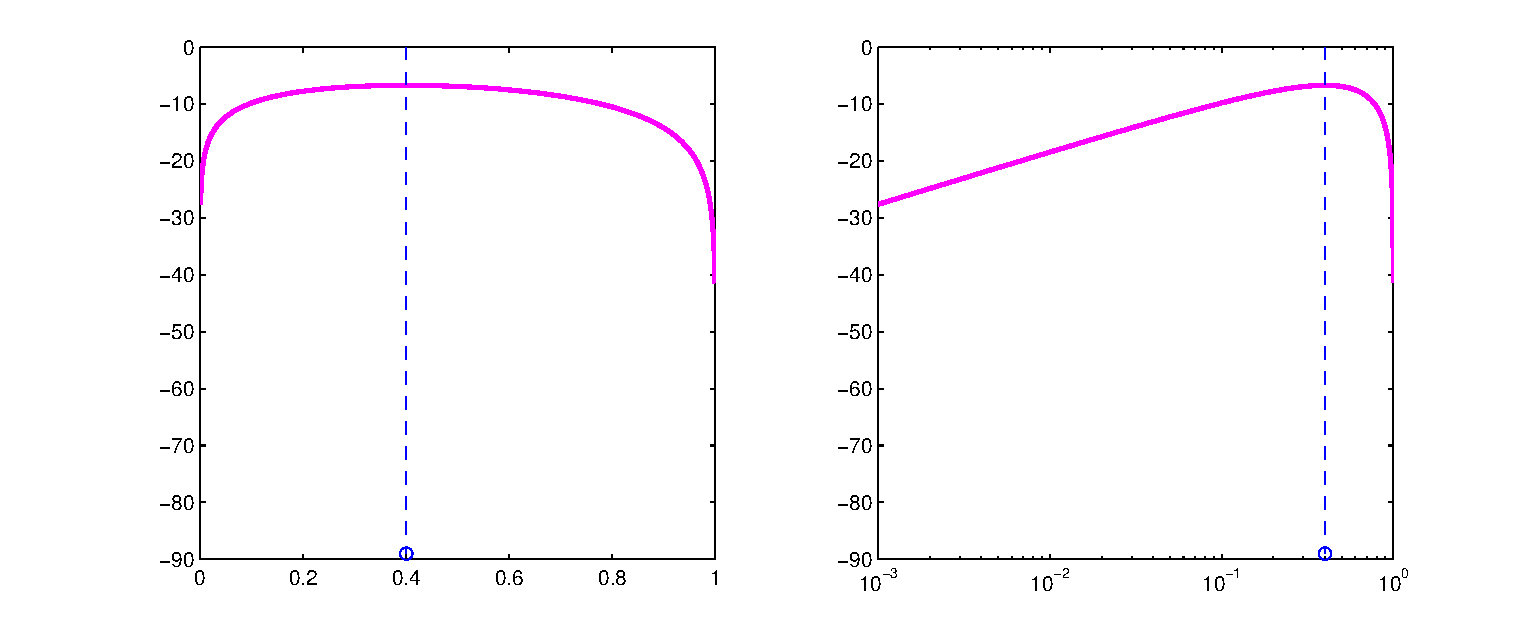
\includegraphics[width=6.5in]{figures/BernoulliMLE}}
\end{figure}


\begin{labwork}[Coin-tossing experiment]\label{LW:BernoulliMLE}
The following script was used to study the coin-tossing experiment in {\sc Matlab}.  The plot of the log-likelihood function and the numerical optimisation of MLE are carried out using {\sc Matlab}'s built-in function {\tt fminbnd} (See \hyperref[F:BernoulliMLE]{Figure \ref*{F:BernoulliMLE}}).

{\VrbMf[label=BernoulliMLE.m]{scripts/BernoulliMLE.m}}

\begin{VrbM}
>> BernoulliMLE
x =     1     0     0     0     1     1     0     0     1     0
t =     4
MLE =    0.4000
Func-count     x          f(x)         Procedure
    1       0.381966      6.73697        initial
    2       0.618034      7.69939        golden
    3       0.236068       7.3902        golden
    4       0.408979      6.73179        parabolic
    5       0.399339      6.73013        parabolic
    6       0.400045      6.73012        parabolic
    7       0.400001      6.73012        parabolic
    8       0.399968      6.73012        parabolic
Optimisation terminated:
 the current x satisfies the termination criteria using OPTIONS.TolX of 1.000000e-04 
NumericalMLE =   0.4000
\end{VrbM}
\end{labwork}

\begin{example}[MLE of an IID $\exponential(\lambda^*)$ experiment]
Let us derive the MLE $\widehat{\Lambda}_n$ of the fixed and possibly unknown $\lambda^*$ for the IID experiment:
$$X_1,\ldots,X_n \overset{IID}{\sim} \exponential(\lambda^*), \qquad \lambda^* \in \BB{\Lambda} = (0,\infty) \enspace .$$
Note that $\BB{\Lambda}$ is the parameter space.

We first obtain the log-likelihood function of $\lambda$ for the data $x_1,x_2,\ldots,x_n \overset{IID}{\sim} \exponential(\lambda)$.
\begin{flalign*}
\ell(\lambda) & := \log(L(x_1,x_2,\ldots,x_n;\lambda)) = \log \left( \prod_{i=1}^n f(x_i;\lambda) \right) 
= \log \left( \prod_{i=1}^n \lambda e^{-\lambda x_i}  \right) \\
&= \log \left( \lambda e^{-\lambda x_1} \cdot \lambda e^{-\lambda x_2}  \cdots \lambda e^{-\lambda x_n}  \right)
= \log \left( \lambda^n e^{-\lambda \sum_{i=1}^n x_i}  \right) \\
&=\log \left( \lambda^n \right) + \log \left( e^{-\lambda \sum_{i=1}^n x_i}  \right) 
= \log \left( \lambda^n \right) -\lambda \sum_{i=1}^n x_i
\end{flalign*}
Now, let us take the derivative with respect to $\lambda$,
\begin{flalign*}
\frac{\partial}{\partial \lambda} \left( \ell(\lambda) \right) 
& :=  \frac{\partial}{\partial \lambda} \left( 
\log \left( \lambda^n \right) -\lambda \sum_{i=1}^n x_i
\right) = \frac{\partial}{\partial \lambda} \left( 
\log \left( \lambda^n \right) \right) -  \frac{\partial}{\partial \lambda} \left( \lambda \sum_{i=1}^n x_i \right) \\
& = \frac{1}{\lambda^n}  \frac{\partial}{\partial \lambda} \left( \lambda^n \right) - \sum_{i=1}^n x_i 
= \frac{1}{\lambda^n}  n \lambda^{n-1}  - \sum_{i=1}^n x_i 
= \frac{n}{\lambda} - \sum_{i=1}^n x_i \enspace .
\end{flalign*}
Next, we set the derivative to $0$, solve for $\lambda$, and set the solution equal to the ML estimate $\widehat{\lambda}_n$.
\begin{flalign*}
0 = \frac{\partial}{\partial \lambda} \left( \ell(\lambda) \right) 
& \iff 0 = \frac{n}{\lambda} - \sum_{i=1}^n x_i \iff \sum_{i=1}^n x_i = \frac{n}{\lambda} \iff \lambda = \frac{n}{\sum_{i=1}^n x_i} \iff \boxed{\widehat{\lambda}_n = \frac{1}{\overline{x}_n}} \enspace .
\end{flalign*}
Therefore, the ML estimate $\widehat{\lambda}_n$ of the unknown rate parameter $\lambda^* \in \BB{\Lambda}$ on the basis of $n$ IID observations $x_1,x_2,\ldots,x_n \overset{IID}{\sim} \exponential(\lambda^*)$ is $1/\overline{x}_n$ and the ML estimator $\widehat{\Lambda}_n=1/\overline{X}_n$.  Let us apply this ML estimator of the rate parameter for the supposedly exponentially distributed waiting times at the on-campus Orbiter bus-stop.
\end{example}

\begin{labwork}[Numerical MLE of $\lambda$ from n IID $\exponential(\lambda)$ RVs]\label{LW:ExponentialMLEOrbiter}
Joshua Fenemore and Yiran Wang collected data on waiting times between buses at an Orbiter bus-stop close to campus and modelled the waiting times as IID $\exponential(\lambda^*)$ RVs (\href{http://www.math.canterbury.ac.nz/~r.sainudiin/courses/STAT218/projects/Stat218StudentProjects2007.pdf}{\url{http://www.math.canterbury.ac.nz/~r.sainudiin/courses/STAT218/projects/Stat218StudentProjects2007.pdf}}).  We can use their data {\tt sampleTimes} to find the MLE of $\lambda^*$ under the assumption that the waiting times $X_1,\ldots,X_{132}$ are IID $\exponential(\lambda^*)$.  We find the ML estimate $\widehat{\lambda}_{132}=0.1102$ and thus the estimated mean waiting time is $1/\widehat{\lambda}_{132}=9.0763$ minutes.  The estimated mean waiting time for a bus to arrive is well within the $10$ minutes promised by the Orbiter bus company.  The following script was used to generate the \hyperref[F:ExponentialMLE]{Figure \ref*{F:ExponentialMLEOrbiter}}:

\VrbMf[label=ExponentialMLEOrbiter.m]{scripts/ExponentialMLEOrbiter.m}

The script output the following in addition to the plot:
\begin{VrbM}
>> ExponentialMLEOrbiter
MLE =    0.1102
MeanEstimate =    9.0763
\end{VrbM}
\end{labwork}

\begin{figure}[htpb]
\caption{Plot of $\log(L(\lambda))$ as a function of the parameter $\lambda$  and the MLE $\widehat{\lambda}_{132}$ of $0.1102$ for Fenemore-Wang Orbiter Waiting Times Experiment from STAT 218 S2 2007.  The density or PDF and the DF at the MLE of $0.1102$ are compared with a histogram and the empirical DF.\label{F:ExponentialMLEOrbiter}}
\centering   \makebox{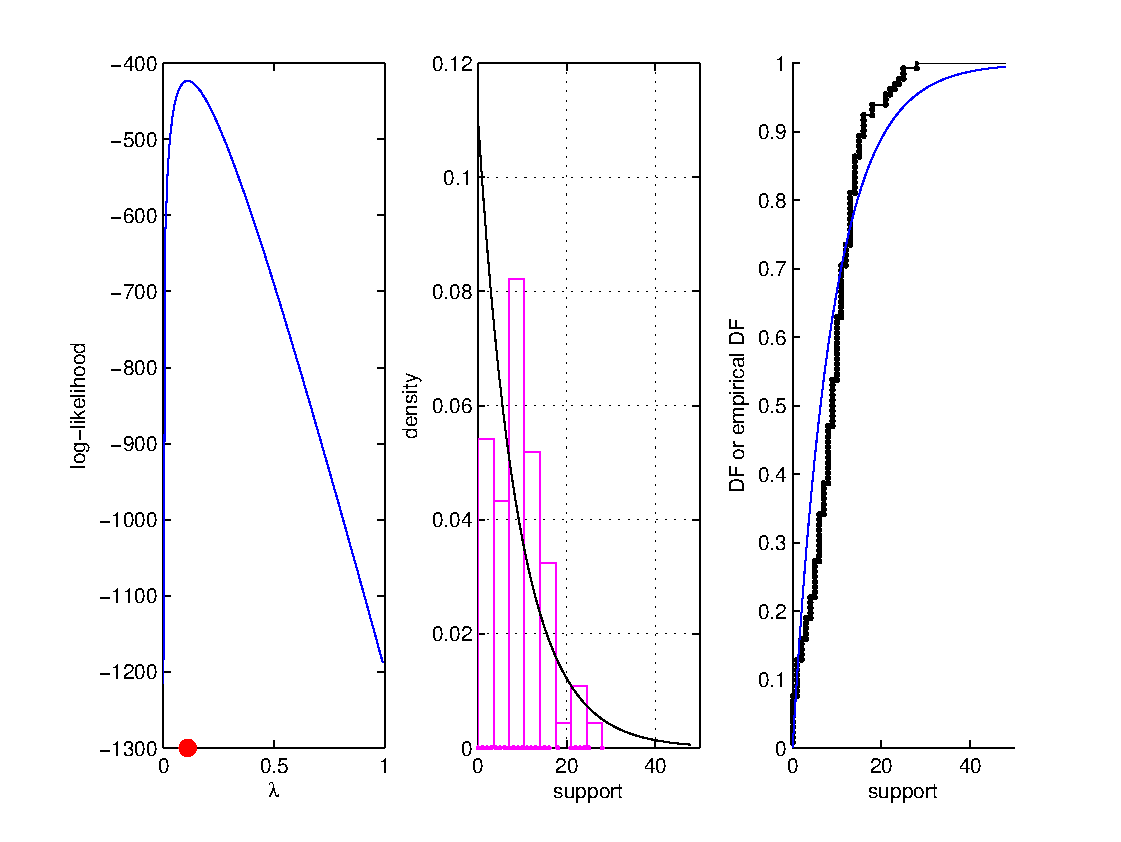
\includegraphics[width=6.5in]{figures/ExponentialMLEOrbiter}}
\end{figure}
Notice how poorly the exponential PDF $f(x;\widehat{\lambda}_{132}=0.1102)$ and the DF $F(x;\widehat{\lambda}_{132}=0.1102)$ based on the MLE fits with the histogram and the empirical DF, respectively.  This is an indication of the inadequacy of our parametric model.  Partly this discrepancy is due to the resolution of the the measurements being confined to whole minutes.  We can overcome this problem by fitting a minute-discretized PMF from the $\exponential(\lambda)$ PDF.  In the next Labwork, we simulate data from an $\exponential(\lambda^*=0.1)$ RV to conduct point estimation in the theoretically ideal setting. 

\begin{labwork}[MLE of the rate parameter for waiting times at my bus stop]\label{LW:ExponentialBusMLE}
Recall \hyperref[LW:Next7Buses]{Labwork~\ref*{LW:Next7Buses}} where you modeled the arrival of buses at a bus stop using the IID $\exponential(\lambda^*=0.1)$ distributed inter-arrival times with a mean of $1/\lambda^*=10$ minutes.  Once again, seed the fundamental sampler by your Student ID (e.g.~if your ID is {\tt 11424620} then type {\tt rand('twister', 11424620);}), just before simulating the inter-arrival times of the next seven buses.  Hand in the following six items:
\begin{enumerate}
\item Waiting times $x_1,x_2,\ldots,x_7$ between arrivals of the next seven buses at your ID-seeded bus stop;
\item A plot of the empirical DF $\widehat{F}_n$  from your (simulated) data $x_1,x_2,\ldots,x_7$.  [You may use the {\sc Matlab} function {\tt ECDF} of  \hyperref[Mf:ECDF]{Labwork \ref*{Mf:ECDF}})];
\item The first, second and third sample quartiles as well as the $0.20^{\text{th}}$ sample quantile for your data $x_1,x_2,\ldots,x_7$.  [You may use the {\sc Matlab} function {\tt qthSampleQuantile} of \hyperref[Mf:qthSampleQuantile]{Labwork \ref*{Mf:qthSampleQuantile}}];
\item Pretending that you did not know the true parameter ($\lambda^*=0.1$) used in the simulation, produce the maximum likelihood estimate (ML estimate) $\widehat{\lambda}_7$ from your seven observations $x_1,x_2,\ldots,x_7$;
\item Plot the log-likelihood function for your data $x_1,x_2,\ldots,x_7$ as a function of the parameter $\lambda$; and
\item Show that you have verified that the numerical optimisation routine {\tt fminbnd} returns the correct ML estimate $\widehat{\lambda}_7$.
\end{enumerate}
 \end{labwork}
 
%\subsubsection*{Summarizing Table of Point Estimators}
%Using the sample mean $\overline{X}_n$ and sample standard deviation $S_n$ defined in \eqref{E:SampleMeanRV} and \eqref{E:SampleStdDevRV}, respectively, we summarise the two point estimators of the parameters of some common distributions below.  For some cases, the MLE is the same as the MME and can be solved analytically.
%\begin{center}
%\begin{table}[htbp]
%\caption{Summary of the Method of Moment Estimator (MME) and the Maximum Likelihood Estimator (MLE) for some IID Experiments. \label{T:MMEMLE}}
%\begin{tabular}{l | r | r}
%\hline
%Statistical Experiment & MLE & MME \\ \hline
%$X_1,X_2,\ldots,X_n \overset{IID}{\sim} \bernoulli(\theta)$ & $\widehat{\theta}=\overline{X}_n$ & same as MLE \\ \hline
%$X_1,X_2,\ldots,X_n \overset{IID}{\sim} \exponential(\lambda)$ & $\widehat{\lambda}={1}/{\overline{X}_n} $ & same as MLE \\ \hline
%$X_1,X_2,\ldots,X_n \overset{IID}{\sim} \normal(\mu,\sigma^2)$ & $\widehat{\mu}=\overline{X}_n, \widehat{\sigma} = \sqrt{\frac{n-1}{n}S^2_n} $ & $\widehat{\mu}=\overline{X}_n, \widehat{\sigma} = S_n $ \\ \hline
%$X_1,X_2,\ldots,X_n \overset{IID}{\sim} \lognormal(\lambda,\zeta)$ & $\widehat{\lambda}=\frac{1}{n}{\sum_{i=1}^n \log(X_i)} $ & $\widehat{\lambda} = \log(\overline{X}_n) - \frac{1}{2} {\widehat{\zeta}} \ ^2$ \\ %\\
% & $\widehat{\zeta} = \sqrt{\frac{1}{n} \sum_{i=1}^n{(\log(X_i)-\widehat{\lambda})^2}} $ & $\widehat{\zeta} = \sqrt{\log \left({S_n^2}/{\overline{X}_n^2} +1 \right)}$ \\
%\hline
%\end{tabular}
%\end{table}
%\end{center}
\begin{figure}[htpb]
\caption{Comparing the $\exponential(\widehat{\lambda}_{6128}= 28.6694)$ PDF and DF with a histogram and empirical DF of the times (in units of days) between earth quakes in  NZ.  The epicentres of $6128$ earth quakes are shown in left panel.\label{F:NZSIEarthQuakesExponentialMLE}}
\centering   \makebox{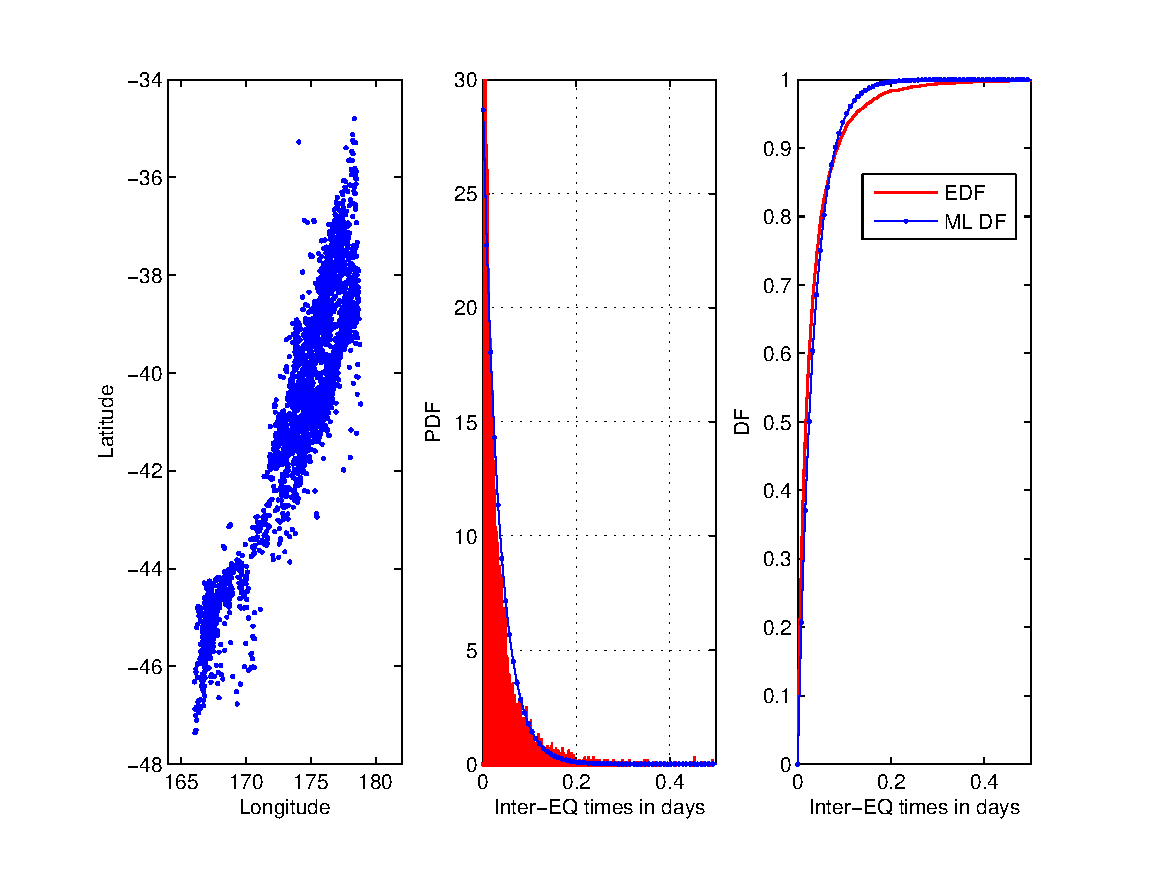
\includegraphics[width=6.5in]{figures/NZSIEarthQuakesExponentialMLE}}
\end{figure}
\begin{labwork}[Time between Earth Quakes in NZ]\label{LW:NZSIEarthQuakesExponentialMLE}  
We model the time between $6128$ earth-quakes in NZ from 18-Jan-2008 02:23:44 to 18-Aug-2008 19:29:29 as:
\[
X_1,X_2,\ldots,X_{6128} \overset{IID}{\sim} \exponential(\lambda^*) \enspace .
\]
Then, the ML estimate of $\lambda^* = 1/\overline{x}_{6128} = 1/0.0349=28.6694$ as computed in the following script:
\VrbMf[label=NZSIEarthQuakesExponentialMLE.m]{scripts/NZSIEarthQuakesExponentialMLE.m}

We first load the data in the text file {\tt earthquakes.csv} into a matrix {\tt EQ}.  Using the {\tt datenum} function in {\sc Matlab} we transform the time stamps into a number starting at zero.  These transformed time stamps are in units of days.  Then we find the times between consecutive events and estimate a histogram.  We finally compute the ML estimate of $\lambda^*$ and super-impose the PDF of the $\exponential(\widehat{\lambda}_{6128}= 28.6694)$ upon the histogram.
\begin{VrbM}
>> NZSIEarthQuakesExponentialMLE
ans =        6128          13

Earth Quakes in NZ between
18-Jan-2008 02:23:44 and18-Aug-2008 19:29:29

SampleMean =    0.0349
MLELambdaHat =   28.6694
\end{VrbM}
Thus, the average time between earth quakes is $0.0349*24*60=50.2560$ minutes.
\end{labwork}

\begin{figure}[htpb]
\caption{The ML fitted ${\rm Rayleigh}(\widehat{\alpha}_{10}= 2)$ PDF and a histogram of the ocean wave heights.\label{F:RayleighOceanHeightsMLE}}
\centering   \makebox{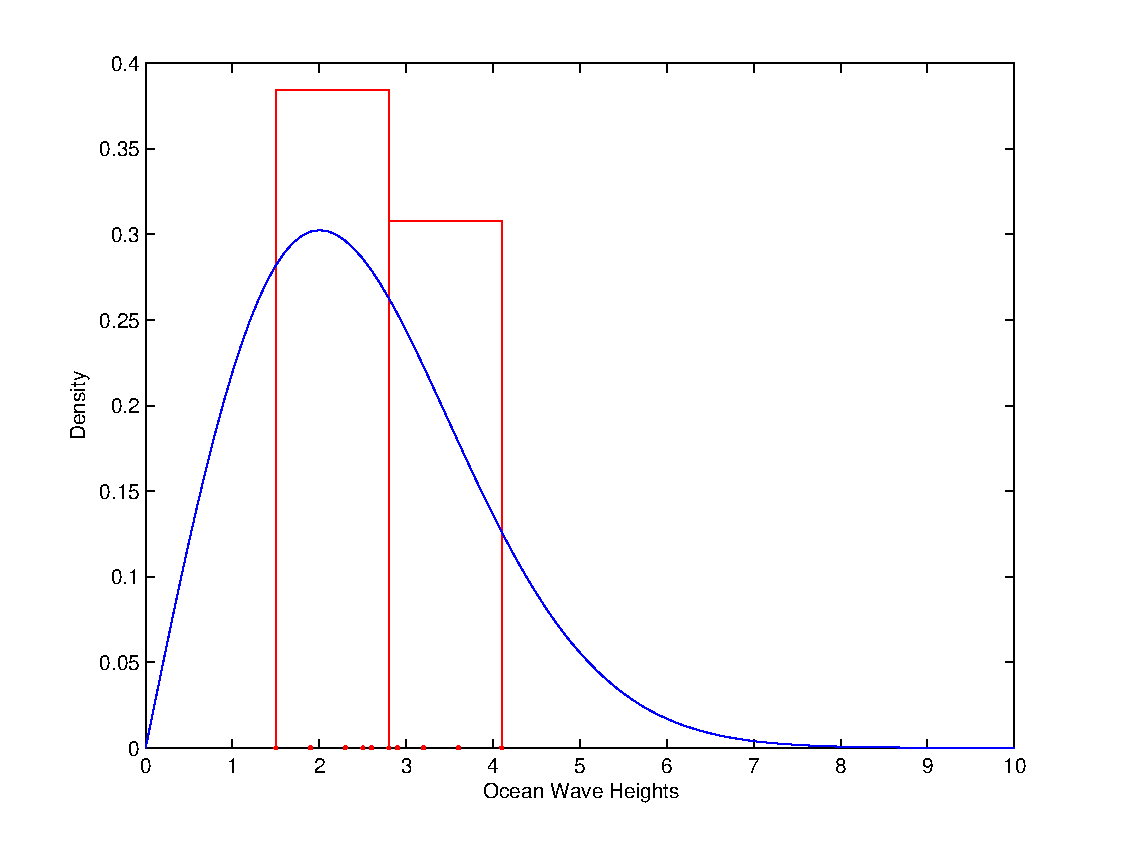
\includegraphics[width=6.5in]{figures/RayleighOceanHeightsMLE}}
\end{figure}
\begin{labwork}[6.7, p.~275 of Ang \& Tang]\label{LW:RayleighOceanHeightsMLE}
The distribution of ocean wave heights, $H$, may be modeled with the ${\rm Rayleigh}(\alpha)$ RV with parameter $\alpha$ and probability density function,
\[
f(h;\alpha) = \frac{h}{\alpha^2} \exp \left({-\frac{1}{2} (h/\alpha)^2}\right), \qquad h \in \Hz := [0,\infty) \ .
\]
The parameter space for $alpha$ is $\BB{A} = (0,\infty)$.  Suppose that the following measurements $h_1,h_2,\ldots,h_{10}$ of wave heights in meters were observed to be
\[
1.50, \  2.80, \ 2.50, \ 3.20, \ 1.90, \ 4.10, \ 3.60, \ 2.60, \ 2.90, \ 2.30 \ ,
\]
respectively.  Under the assumption that the $10$ samples are IID realisations from a ${\rm Rayleigh}(\alpha^*)$ RV with a fixed and unknown parameter $\alpha^*$, find the ML estimate $\widehat{\alpha}_{10}$ of $\alpha^*$.

We first obtain the log-likelihood function of $\alpha$ for the data $h_1,h_2,\ldots,h_n \overset{IID}{\sim} {\rm Rayleigh}(\alpha)$.
\begin{flalign*}
\ell(\alpha) & := \log(L(h_1,h_2,\ldots,h_n;\alpha)) = \log \left( \prod_{i=1}^n f(h_i;\alpha) \right) = \sum_{i=1}^n \log(f(h_i; \alpha))\\
& = \sum_{i=1}^n \log \left( \frac{h_i}{\alpha^2} e^{-\frac{1}{2} (h_i/\alpha)^2} \right) 
=  \sum_{i=1}^n \left( \log(h_i) - 2 \log(\alpha)  {-\frac{1}{2} (h_i/\alpha)^2} \right) \\
& = \sum_{i=1}^n \left( \log(h_i) \right) - 2 n \log(\alpha) - \sum_{i=1}^n \left(  \frac{1}{2} h_i^2 \alpha^{-2} \right) 
\end{flalign*}
Now, let us take the derivative with respect to $\alpha$,
\begin{flalign*}
\frac{\partial}{\partial \alpha} \left( \ell(\alpha) \right) 
& :=  \frac{\partial}{\partial \alpha} \left( \sum_{i=1}^n \left( \log(h_i) \right) - 2 n \log(\alpha) - \sum_{i=1}^n \left(  \frac{1}{2} h_i^2 \alpha^{-2} \right) \right) \\
& = \frac{\partial}{\partial \alpha} \left( \sum_{i=1}^n \left( \log(h_i) \right) \right) -  \frac{\partial}{\partial \alpha} \left( 2 n \log(\alpha) \right) -  \frac{\partial}{\partial \alpha} \left( \sum_{i=1}^n \left(  \frac{1}{2} h_i^2 \alpha^{-2} \right) \right) \\
& = 0 - 2n \frac{1}{\alpha} - \sum_{i=1}^n \left(  \frac{1}{2} h_i^2 (-2 \alpha^{-3}) \right)
= - 2n \alpha^{-1} + \alpha^{-3} \sum_{i=1}^n \left( h_i^2  \right)
\end{flalign*}
Next, we set the derivative to $0$, solve for $\alpha$, and set the solution equal to the ML estimate $\widehat{\alpha}_n$.
\begin{flalign*}
0 = \frac{\partial}{\partial \alpha} \left( \ell(\alpha) \right) 
& \iff 0 = - 2n \alpha^{-1} + \alpha^{-3} \sum_{i=1}^n h_i^2 \iff 2n \alpha^{-1} = \alpha^{-3} \sum_{i=1}^n h_i^2 \\
& \iff 2n \alpha^{-1} \alpha^{3} = \sum_{i=1}^n h_i^2 \iff \alpha^{2} = \frac{1}{2n} \sum_{i=1}^n h_i^2
\iff \widehat{\alpha}_n = \sqrt{  \frac{1}{2n} \sum_{i=1}^n h_i^2 }
\end{flalign*}
Therefore, the ML estimate of the unknown $\alpha^* \in \BB{A}$ on the basis of our $10$ observations $h_1,h_2,\ldots,h_{10}$ of wave heights is
\begin{flalign*}
\widehat{\alpha}_{10} & =  \sqrt{  \frac{1}{2*10} \sum_{i=1}^{10} h_i^2 } \\
& = \sqrt{ \frac{1}{20} \left( 1.50^2 + 2.80^2 + 2.50^2 + 3.20^2 + 1.90^2 + 4.10^2 + 3.60^2 + 2.60^2 + 2.90^2 + 2.30^2 \right)} \approxeq 2
\end{flalign*}
We use the following script file to compute the MLE $\widehat{\alpha}_{10}$ and plot the PDF at $\widehat{\alpha}_{10}$ in \hyperref[F:RayleighOceanHeightsMLE]{Figure~\ref*{F:RayleighOceanHeightsMLE}}.
\VrbMf[label=RayleighOceanHeightsMLE.m]{scripts/RayleighOceanHeightsMLE.m}
\begin{VrbM}
>> RayleighOceanHeightsMLE
AlphaHat =    2.0052
\end{VrbM}
\end{labwork}

%\begin{labwork}
%Choose some parameter $p\in[0,1]$ and some sample size $n$.  Then, using the {\sc Matlab} expression {\tt floor(rand(1,n)+p)} (See \hyperref[SIM:Bernoulli]{Simulation~\ref*{SIM:Bernoulli}}) simulate $n$ IID $\bernoulli(p)$ RVs $X_1,X_2,\ldots,X_n$.  Once you have generated the data, pretend that you don't know the $p$ used in your simulation and estimate $p$ using the sample mean estimator we have seen in \hyperref[EX:EstimatePFromNIIDBernoulliTrials]{Example~\ref*{EX:EstimatePFromNIIDBernoulliTrials}},  That is, compute the estimate $\widehat{p}_n=n^{-1}\sum_{i=1}^n x_i$ and also the approximate $95\%$ Normal-based confidence interval $C_n = \widehat{p}_n \pm 1.96 \sqrt{\frac{\widehat{p}_n(1-\widehat{p}_n)}{n}}$.

%For each value of $p \in [0, 1/100, 1/10, 2/10, 3/10, 4/10, 5/10, 6/10, 7/10, 8/10, 9/10, 9/100, 1]$,  generate $n$ IID $\bernoulli(p)$ samples where $n$ ranges in $\{10^i: i =1,2,3,4,5 \}$ and estimate $p$ from the simulated data of different sample sizes.  Do you intuitively agree with the behavior of the confidence intervals, in terms of the changes in their widths, as $n$ gets large for each of the fixed $p$'s ?  Is the point estimate $\widehat{p}_n$ approaching the $p$ from which the data were simulated for each of the fixed $p$'s as $n$ gets large ?
%For each value of $p$ as before, generate, say $1000$ data sets each of sample size $n \in \{10^i: i =1,2,3,4,5 \}$ and empirically study the coverage properties of the estimator.  That is, for each $p$ and $n$, find what fraction of the Normal-based  $95\%$ confidence intervals constructed from each of the $1000$ replicate data sets actually contain the parameter $p$ that they were simulated from.  Try to explain why coverage properties are both a function of how close $p$ is to the boundary of the the parameter space $[0,1]$ and the sample size $n$.  [Inspired by Russell Gribble]
%\end{labwork}

\section{Properties of the Maximum Likelihood Estimator}\label{S:PropsMLE}
Next, we list some nice properties of the ML Estimator $\widehat{\Theta}_n$ for the fixed and possibly unknown $\theta^* \in \BB{\Theta}$.
\begin{enumerate}
\item The ML Estimator is asymptotically consistent, i.e.~
$\widehat{\Theta}_n \overset{P}{\longrightarrow} \theta^*$.
\item The ML Estimator is asymptotically normal, i.e.~
$(\widehat{\Theta}_n - \theta^*) / \widehat{se}_n \rightsquigarrow \normal(0,1)$.
\item The estimated standard error of the ML Estimator, $\widehat{\mathsf{se}}_n$, can usually be computed analytically using the \hyperref[S:FisherInfo]{\bf Fisher Information}.
\item Because of the previous two properties, the $1-\alpha$ confidence interval can also be computed analytically as $\widehat{\Theta}_n \pm z_{\alpha/2} \widehat{\mathsf{se}}_n$.
\item The ML Estimator is {\bf equivariant}, i.e.~$\widehat{\psi}_n=g(\widehat{\theta}_n)$ is the ML Estimate of $\psi^*=g(\theta^*)$, for some smooth function $g(\theta)=\psi: \BB{\Theta} \to \BB{\Psi}$.  
\item We can also obtain the estimated standard error of the estimator 
$\widehat{\Psi}_n$ of $\psi^* \in \BB{\Psi}$ via the \hyperref[S:DeltaMethod]{\bf Delta Method}.
\item The ML Estimator is {\bf asymptotically optimal} or {\bf efficient}.  This means that the MLE has the smallest variance among the well-behaved class of estimators as the sample size gets larger.
\item ML Estimator is close to the Bayes estimator (obtained in the Bayesian inferential paradigm).
\end{enumerate}

\section{Fisher Information}\label{S:FisherInfo}
Let $X_1,X_2,\ldots,X_n \overset{IID}{\sim} f(X_1;\theta)$.  Here, $f(X_1;\theta)$ is the probability density function (pdf) or the probability mass function (pmf) of the RV $X_1$.  Since all RVs are identically distributed, we simply focus on $X_1$ without loss of generality.
\begin{definition}[Fisher Information]\label{D:FisherInfo}
The {\bf score function} of an RV $X$ for which the density is parameterised by $\theta$ is defined as:
\[
\mathscr{S}(X;\theta) := \frac{\partial log f(X;\theta)}{\partial \theta}, \qquad \text{and} \quad 
\E_{\theta} (\mathscr{S}(X;\theta))=0 \ .
\]
The {\bf Fisher Information} is
\begin{equation}\label{E:FisherInfo}
I_n := \V_{\theta} \left( \sum_{i=1}^n \mathscr{S}(X_i;\theta) \right) 
=  \sum_{i=1}^n \V_{\theta} \left( \mathscr{S}(X_i;\theta) \right) 
= n I_1(\theta),
\end{equation}
where $I_1$ is the Fisher Information of just one of the RVs $X_i$,e.g.~$X$:
\begin{eqnarray}
I_1 (\theta) &:=& \V_{\theta} \left( \mathscr{S}(X;\theta) \right) 
= \E_{\theta} \left(  \mathscr{S}^2(X,\theta) \right) \notag \\
&=& - \E_{\theta} \left(  \frac{\partial^2 log f(X;\theta)}{\partial^2 \theta} \right)
=
\begin{cases}
-\sum_{x \in \Xz}  \left( \frac{\partial^2 \log f(x;\theta)}{\partial^2 \theta} \right) f(x;\theta)  & \text{for discrete $X$}\\
-\int_{x \in \Xz}  \left( \frac{\partial^2 \log f(x;\theta)}{\partial^2 \theta} \right) f(x;\theta) dx  & \text{for continuous $X$} \qquad \label{E:FisherInfo1}
\end{cases}
\end{eqnarray}
\end{definition}
Next, we give a {\bf general method} for obtaining:
\begin{enumerate}
\item
The standard error $\mathsf{se}_n(\widehat{\Theta}_n)$ of {\bf any} maximum likelihood estimator $\widehat{\Theta}_n$ of the possibly unknown and fixed parameter of interest $\theta^* \in \BB{\Theta}$, and
\item The $1-\alpha$ confidence interval for $\theta^*$.
\end{enumerate}

\begin{prop}[Asymptotic Normality of the ML Estimator \& Confidence Intervals]
Let $\widehat{\Theta}_n$ be the maximum likelihood estimator of $\theta^* \in \BB{\Theta}$ with standard error $\mathsf{se}_n := \sqrt{\V_{\theta^*} (\widehat{\Theta}_n)}$.  Under appropriate regularity conditions, the following propositions are true:
\begin{enumerate}
\item The standard error $\mathsf{se}_n$ can be approximated by the side of a square whose area is the inverse Fisher Information at $\theta^*$, and the distribution of $\widehat{\Theta}_n$ approaches that of the $\normal(\theta^*, \mathsf{se}_n^2)$ distribution as the samples size $n$ gets larger.  In other terms:
\[
\mathsf{se}_n \approxeq \sqrt{1/I_n(\theta^*)} \qquad \text{and} \quad \frac{\widehat{\Theta}_n-\theta^*}{\mathsf{se}_n} \rightsquigarrow \normal(0,1)
\]
\item The approximation holds even if we substitute the ML Estimate $\widehat{\theta}_n$ for $\theta^*$ and use the estimated standard error $\widehat{\mathsf{se}}_n$ instead of $\mathsf{se}_n$.  Let $\widehat{\mathsf{se}}_n = \sqrt{1/I_n(\widehat{\theta}_n)}$.  Then:
\[
 \frac{\widehat{\Theta}_n-\theta^*}{\widehat{\mathsf{se}}_n} \rightsquigarrow \normal(0,1)
\]
\item Using the fact that $\widehat{\Theta}_n \rightsquigarrow \normal(\theta^*,\widehat{se}_n^2)$, we can construct the estimate of an approximate Normal-based $1-\alpha$ confidence interval as:
\[
C_n  =[\underline{C}_n, \overline{C}_n]= [\widehat{\theta}_n - z_{\alpha/2} \widehat{se}_n, \widehat{\theta}_n + z_{\alpha/2} \widehat{\mathsf{se}}_n]= \widehat{\theta}_n \pm z_{\alpha/2} \widehat{\mathsf{se}}_n
\]
\end{enumerate}
\end{prop}
Now, let us do an example.
\begin{example}[MLE and Confidence Interval for the IID $\poisson(\lambda)$ experiment]
Suppose the fixed parameter $\lambda^* \in \BB{\Lambda} = (0,\infty)$ is unknown.  Let $X_1,X_2,\ldots,X_n \overset{IID}{\sim} \poisson(\lambda^*)$.  We want to find the ML Estimate $\widehat{\lambda}_n$ of $\lambda^*$ and produce a $1-\alpha$ confidence interval for $\lambda^*$.

The MLE can be obtained as follows:

The likelihood function is:
\[
L(\lambda) := L(x_1,x_2,\ldots,x_n; \lambda) = \prod_{i=1}^n f(x_i;\lambda) = \prod_{i=1}^n e^{-\lambda} \frac{\lambda^x_i}{x_i!}
\]
Hence, the log-likelihood function is:
\begin{eqnarray}
\ell(\theta) := \log(L(\lambda)) 
&=&  \log \left( \prod_{i=1}^n e^{-\lambda} \frac{\lambda^{x_i}}{x_i!} \right) =  \sum_{i=1}^n \log \left(  e^{-\lambda} \frac{\lambda^{x_i}}{x_i!} \right) 
=  \sum_{i=1}^n \left( \log (e^{-\lambda}) + \log( \lambda^{x_i}) - \log({x_i!}) \right)  \notag \\
&=& \sum_{i=1}^n \left({-\lambda} + x_i \log( \lambda) - \log({x_i!}) \right) 
= \sum_{i=1}^n {-\lambda} + \sum_{i=1}^n x_i \log( \lambda) - \sum_{i=1}^n \log({x_i!})  \notag \\
&=& n ( {-\lambda}) + \log( \lambda) \left( \sum_{i=1}^n x_i \right) - \sum_{i=1}^n \log({x_i!})  \notag 
\end{eqnarray}
Next, take the derivative of $\ell(\lambda)$:
\[
\frac{\partial}{\partial \lambda} \ell (\lambda) 
= \frac{\partial}{\partial \lambda} \left(  n ( {-\lambda}) + \log( \lambda) \left( \sum_{i=1}^n x_i \right) - \sum_{i=1}^n \log({x_i!})  \right)
= n(-1) + \frac{1}{\lambda} \left( \sum_{i=1}^n x_i \right) + 0
\]
and set it equal to $0$ to solve for $\lambda$, as follows:
\[
0 = n(-1) + \frac{1}{\lambda} \left( \sum_{i=1}^n x_i \right) + 0 \iff n = \frac{1}{\lambda} \left( \sum_{i=1}^n x_i \right) \iff \lambda =  \frac{1}{n} \left( \sum_{i=1}^n x_i \right) = \overline{x}_n
\]
Finally, the ML Estimator of $\lambda^*$ is $\widehat{\Lambda}_n = \overline{X}_n$ and the ML estimate is $\widehat{\lambda}_n = \overline{x}_n$.

Now, we want an $1-\alpha$ confidence interval for $\lambda^*$ using the $\widehat{\mathsf{se}}_n \approxeq \sqrt{1/I_n(\widehat{\lambda}_n)}$ that is based on the Fisher Information $I_n(\lambda) = n I_1(\lambda)$ given in \eqref{E:FisherInfo}.  We need $I_1$ given in \eqref{E:FisherInfo1}.  Since $X_1,X_2,\ldots,X_n \sim \poisson(\lambda)$, we have discrete RVs:
\[
I_1 = -\sum_{x \in \Xz}  \left( \frac{\partial^2 \log (f(x;\lambda))}{\partial^2 \lambda} \right) f(x;\lambda) = -\sum_{x =0}^{\infty}  \left( \frac{\partial^2 \log (f(x;\lambda))}{\partial^2 \lambda} \right) f(x;\lambda)
\]
First find 
\begin{eqnarray}
\frac{\partial^2 \log (f(x;\lambda))}{\partial^2 \lambda}
&=& \frac{\partial}{\partial \lambda} \left( \frac{\partial} {\partial \lambda} \log \left(  f(x;\lambda) \right
) \right)
=  \frac{\partial}{\partial \lambda} \left( \frac{\partial} {\partial \lambda} \log \left( e^{-\lambda} \frac{\lambda^x}{x!} \right) \right) \notag \\
&=& \frac{\partial}{\partial \lambda} \left( \frac{\partial} {\partial \lambda} \left( -\lambda + x \log(\lambda)-\log({x!}) \right) \right)
= \frac{\partial}{\partial \lambda} \left( -1 + \frac{x}{\lambda}-0 \right)
= -\frac{x}{\lambda^2} \notag
\end{eqnarray}
\end{example}
Now, substitute the above expression into the right-hand side of $I_1$ to obtain:
\[
I_1= - \sum_{x=0}^{\infty} \left( -\frac{x}{\lambda^2} \right) f(x;\lambda)
= \frac{1}{\lambda^2} \sum_{x=0}^{\infty} \left( x \right) f(x;\lambda)
= \frac{1}{\lambda^2} \sum_{x=0}^{\infty} \left( x \right) e^{-\lambda} \frac{\lambda^x}{x!} 
=  \frac{1}{\lambda^2} \E_{\lambda}(X)
= \frac{1}{\lambda^2} \lambda
=\frac{1}{\lambda}
\]
In the third-to-last step above, we recognise the sum as the expectation of the $\poisson(\lambda)$ RV $X$, namely $\E_{\lambda}(X)=\lambda$.  Therefore, the estimated standard error is:
\[
\widehat{\mathsf{se}}_n \approxeq \sqrt{1/I_n(\widehat{\lambda}_n)}
= \sqrt{1/(n I_1(\widehat{\lambda}_n))}
= \sqrt{1/(n (1/\widehat{\lambda}_n))}
= \sqrt{\widehat{\lambda}_n/n}
\]
and the approximate $1-\alpha$ confidence interval is
\[
\widehat{\lambda}_n \pm z_{\alpha/2} \widehat{\mathsf{se}}_n 
= \widehat{\lambda}_n \pm z_{\alpha/2} \sqrt{\widehat{\lambda}_n/n}
\]

Thus, using the MLE and the estimated standard error via the Fisher Information, we can carry out point estimation and confidence interval construction in {\bf most} parametric families of RVs encountered in typical engineering applications.  

\begin{example}[Fisher Information of the $\bernoulli$ Experiment]\label{EX:BernoulliFisherInfo}
Suppose $X_1,X_2,\ldots,X_n \overset{IID}{\sim}$ $\bernoulli(\theta^*)$.  Also, suppose that $\theta^* \in \BB{\Theta} = [0,1]$ is unknown.  We have already shown in \hyperref[EX:CoinTossingML]{Example~\ref*{EX:CoinTossingML}} that the ML estimator of $\theta^*$ is $\widehat{\theta}_n = \overline{X}_n$.  Using the identity:
\[
\widehat{\mathsf{se}}_n = \frac{1}{\sqrt{I_n(\widehat{\theta}_n)}}
\]
(1) we can compute $\widehat{\mathsf{se}}_n(\widehat{\Theta}_n)$, the estimated standard error  of the unknown parameter $\theta^*$ as follows:
\begin{flalign*}
\widehat{\mathsf{se}}_n (\widehat{\Theta}_n) &= \frac{1}{\sqrt{I_n(\widehat{\theta}_n)}} =   \frac{1}{\sqrt{n I_1(\widehat{\theta}_n)}} \ .
\end{flalign*}
So, we need to first compute $I_1(\theta)$, the Fisher Information of one sample.  Due to \eqref{E:FisherInfo1} and the fact that the $\bernoulli(\theta^*)$ distributed RV $X$ is discrete with probability mass function $f(x;\theta)=\theta^{x} (1-\theta)^{1-x}$, for $x\in \Xz := \{0,1\}$, we have,
\begin{flalign*}
I_1(\theta) &= - \E_{\theta} \left(  \frac{\partial^2 log f(X;\theta)}{\partial^2 \theta} \right) = - \sum_{x \in \Xz = \{0,1\}} \left( \frac{\partial^2 \log \left( \theta^{x} (1-\theta)^{1-x} \right)}{\partial^2 \theta} \right) \theta^{x} (1-\theta)^{1-x} \\
\end{flalign*}
Next, let us compute,
\begin{flalign*}
\frac{\partial^2 \log \left( \theta^{x} (1-\theta)^{1-x} \right)}{\partial^2 \theta} & :=
\frac{\partial}{\partial \theta} \left( \frac{\partial}{\partial \theta} \left( \log \left( \theta^{x} (1-\theta)^{1-x} \right) \right) \right) = 
\frac{\partial}{\partial \theta} \left( \frac{\partial}{\partial \theta} \left( x \log(\theta) + (1-x) \log(1-\theta)  \right) \right) \\
& = \frac{\partial}{\partial \theta} \left(  x \theta^{-1} + (1-x)(1-\theta)^{-1} (-1)  \right) 
=\frac{\partial}{\partial \theta} \left(  x \theta^{-1} - (1-x)(1-\theta)^{-1}  \right)  \\
&=  x (-1) \theta^{-1-1} - (1-x) (-1) (1-\theta)^{-1-1} (-1)
= - x \theta^{-2} - (1-x) (1-\theta)^{-2}
\end{flalign*}
Now, we compute the expectation $I_1$, i.e.~the sum over the two possible values of $x\in\{0,1\}$,
\begin{flalign*}
I_1(\theta) &= - \sum_{x \in \Xz = \{0,1\}} \left( \frac{\partial^2 \log \left( \theta^{x} (1-\theta)^{1-x} \right)}{\partial^2 \theta} \right) \theta^{x} (1-\theta)^{1-x} \\
& = - \left( \left(- 0 \ \theta^{-2} - (1-0) (1-\theta)^{-2} \right) \theta^{0} (1-\theta)^{1-0} + \left( - 1 \ \theta^{-2} - (1-1) (1-\theta)^{-2} \right) \theta^{1} (1-\theta)^{1-1} \right) \\
& = - \left( \left(0 - 1 (1-\theta)^{-2} \right) \ 1 \ (1-\theta)^1 + \left( - \theta^{-2} - 0  \right) \theta^1 \ 1 \right) 
=  (1-\theta)^{-2} (1-\theta)^1 +  \theta^{-2} \theta^1 \\
& = (1-\theta)^{-1} +  \theta^{-1}  = \frac{1}{1-\theta} + \frac{1}{\theta} 
= \frac{\theta}{\theta (1-\theta)} +  \frac{1-\theta}{\theta (1-\theta)} 
= \frac{\theta+(1 - \theta)}{\theta (1-\theta)} = \frac{1}{\theta (1-\theta)}
\end{flalign*}
Therefore, the desired estimated standard error of our estimator, can be obtained by substituting the ML estimate $\widehat{\theta}_n=\overline{x}_n := n^{-1}\sum_{i=1}^n x_i$ of the unknown $\theta^*$ as follows:
\begin{flalign*}
\widehat{\mathsf{se}}_n(\widehat{\theta}_n) = \frac{1}{\sqrt{I_n(\widehat{\theta}_n)}} 
 = \frac{1}{\sqrt{n I_1(\widehat{\theta}_n)}}
 = \sqrt{\frac{1}{n \frac{1}{\widehat{\theta}_n (1-\widehat{\theta}_n)} }} 
= \sqrt{\frac{\widehat{\theta}_n(1-\widehat{\theta}_n)}{n}} 
= \sqrt{\frac{\overline{x}_n(1-\overline{x}_n)}{n}}  \ .
\end{flalign*}
(2) Using $\widehat{\mathsf{se}}_n(\widehat{\theta}_n)$ we can construct an approximate $95\%$ confidence interval $C_n$ for $\theta^*$, due to the asymptotic normality of the ML estimator of $\theta^*$, as follows:
\[
C_n = \widehat{\theta}_n \pm 1.96 \sqrt{\frac{\widehat{\theta}_n(1-\widehat{\theta}_n)}{n}}
= \overline{x}_n \pm 1.96 \sqrt{\frac{\overline{x}_n(1-\overline{x}_n)}{n}}
\]
Recall that $C_n$ is the realisation of a random set based on your observed samples or data  $x_1,x_2,\ldots,x_n$.   Furthermore, $C_n$'s construction procedure ensures the engulfing of the unknown $\theta^*$ with probability approaching $0.95$ as the sample size $n$ gets large.

%(3) Flip any New Zealand coin as identically and independently as possible exactly $30$ times and record the outcomes ($1$ for heads and $0$ for tails).  Report the ML point estimate and the $95\%$ confidence interval from your data.  Do you think that the way you have flipped your coin and the outcomes you have witnessed can hint at the fairness ($\theta^*=0.5$) or unfairness ($\theta^*\neq0.5$) of the coin.  Write a couple of sentences to make your case.    [Take the time to flip coins this many times in a row, if you have not done so already.  Be honest and really do it.  I flipped an American quarter $100$ times to produce the data in \hyperref[EX:EstimatePFromNIIDBernoulliTrials]{Example \ref*{EX:EstimatePFromNIIDBernoulliTrials}}].
\end{example}

\begin{example}[[Fisher Information of the $\exponential$ Experiment]]\label{EX:ExponentialFisherInfo}
Let us get our hands dirty with a continuous RV next.  Let $X_1,X_2,\ldots,X_n \overset{IID}{\sim} \exponential(\lambda^*)$.  We saw that the ML estimator of $\lambda^* \in \BB{\Lambda}=(0,\infty)$ is $\widehat{\Lambda}_n = 1/\overline{X}_n$ and its ML estimate is $\widehat{\lambda}_n=1/\overline{x}_n$, where $x_1,x_2,\ldots,x_n$ are our observed data.

(1) Let us obtain the Fisher Information $I_n$ for this experiment to find the standard error:
\[
\widehat{\mathsf{se}}_n(\widehat{\Lambda}_n) = \frac{1}{\sqrt{I_n(\widehat{\lambda}_n)}}
= \frac{1}{\sqrt{n I_1(\widehat{\lambda}_n)}}
\]
and construct an approximate $95\%$ confidence interval for $\lambda^*$ using the asymptotic normality of its ML estimator $\widehat{\Lambda}_n$.  

So, we need to first compute $I_1(\theta)$, the Fisher Information of one sample.  Due to \eqref{E:FisherInfo1} and the fact that the $\exponential(\lambda^*)$ distributed RV $X$ is continuous with probability density function $f(x;\lambda)=\lambda e^{-\lambda x}$, for $x\in \Xz := [0,\infty)$, we have,
\begin{flalign*}
I_1(\theta) &= - \E_{\theta} \left(  \frac{\partial^2 log f(X;\theta)}{\partial^2 \theta} \right) = - \int_{x \in \Xz = [0,\infty)} \left( \frac{\partial^2 \log \left( \lambda e^{-\lambda x} \right)}{\partial^2 \lambda} \right) \lambda e^{-\lambda x} \ dx
\end{flalign*}
Let us compute the above integrand next.
\begin{flalign*}
\frac{\partial^2 \log \left( \lambda e^{-\lambda x} \right)}{\partial^2 \lambda}
&:= 
\frac{\partial}{\partial \lambda} \left( \frac{\partial}{\partial \lambda} \left( \log \left( \lambda e^{-\lambda x} \right)   \right) \right)
= \frac{\partial}{\partial \lambda} \left( \frac{\partial}{\partial \lambda} \left( \log(\lambda) + \log(e^{-\lambda x} \right) \right) \\
&= \frac{\partial}{\partial \lambda} \left( \frac{\partial}{\partial \lambda} \left( \log(\lambda) -\lambda x \right) \right) 
= \frac{\partial}{\partial \lambda} \left( {\lambda}^{-1} - x \right) = - \lambda^{-2} - 0 = -\frac{1}{\lambda^2}
\end{flalign*}
Now, let us evaluate the integral by recalling that the expectation of the constant $1$ is 1 for any RV $X$ governed by some parameter, say $\theta$.  For instance when $X$ is a continuous RV, $\E_{\theta}(1) = \int_{x \in \Xz} 1 \ f(x;\theta) =  \int_{x \in \Xz} \ f(x;\theta) = 1$.  Therefore, the Fisher Information of one sample is
\begin{flalign*}
I_1(\theta) = - \int_{x \in \Xz = [0,\infty)} \left( \frac{\partial^2 \log \left( \lambda e^{-\lambda x} \right)}{\partial^2 \lambda} \right) \lambda e^{-\lambda x} \ dx
 &=  - \int_{0}^{\infty} \left(-\frac{1}{\lambda^2} \right) \lambda e^{-\lambda x} \ dx \\
& = -  \left(-\frac{1}{\lambda^2} \right) \int_{0}^{\infty} \lambda e^{-\lambda x} \ dx = \frac{1}{\lambda^2} \ 1 = \frac{1}{\lambda^2}
\end{flalign*}
Now, we can compute the desired estimated standard error, by substituting in the ML estimate $\widehat{\lambda}_n = 1/(\overline{x}_n) := 1 / \left( \sum_{i=1}^n x_i \right)$ of $\lambda^*$, as follows:
\[
\widehat{\mathsf{se}}_n(\widehat{\Lambda}_n) = \frac{1}{\sqrt{I_n(\widehat{\lambda}_n)}}
= \frac{1}{\sqrt{n I_1(\widehat{\lambda}_n)}} 
= \frac{1}{\sqrt{n \frac{1}{\widehat{\lambda}_n^2} }}
= \frac{\widehat{\lambda}_n}{\sqrt{n}}
= \frac{1}{\sqrt{n} \ \overline{x}_n}
\]
Using $\widehat{\mathsf{se}}_n(\widehat{\lambda}_n)$ we can construct an approximate $95\%$ confidence interval $C_n$ for $\lambda^*$, due to the asymptotic normality of the ML estimator of $\lambda^*$, as follows:
\[
C_n 
= \widehat{\lambda}_n \pm 1.96 \frac{\widehat{\lambda}_n}{\sqrt{n}}
= \frac{1}{\overline{x}_n} \pm 1.96 \frac{1}{\sqrt{n} \ \overline{x}_n} \enspace .
\]
Let us compute the ML estimate and the $95\%$ confidence interval for the rate parameter for the waiting times at the Orbiter bus-stop (see \hyperref[LW:ExponentialMLEOrbiter]{labwork~\ref*{LW:ExponentialMLEOrbiter}}).  The sample mean $\overline{x}_{132}=9.0758$ and the ML estimate is:
$$\widehat{\lambda}_{132}=1/\overline{x}_{132}=1/9.0758=0.1102 \enspace ,$$
and the $95\%$ confidence interval is:  
\[
C_n 
= \widehat{\lambda}_{132} \pm 1.96 \frac{\widehat{\lambda}_{132}}{\sqrt{132}}
= \frac{1}{\overline{x}_{132}} \pm 1.96 \frac{1}{\sqrt{132} \ \overline{x}_{132}} = 0.1102 \pm 1.96 \cdot 0.0096 = [0.0914, 0.1290] \enspace .
\]
Notice how poorly the exponential PDF $f(x;\widehat{\lambda}_{132}=0.1102)$ and the DF $F(x;\widehat{\lambda}_{132}=0.1102)$ based on the MLE fits with the histogram and the empirical DF, respectively, in \hyperref[F:ExponentialMLECIOrbiter]{Figure~\ref*{F:ExponentialMLECIOrbiter}}, despite  taking the the confidence interval into account.  This is a further indication of the inadequacy of our parametric model.
\end{example}

\begin{figure}[htpb]
\caption{Plot of $\log(L(\lambda))$ as a function of the parameter $\lambda$, the MLE 
$\widehat{\lambda}_{132}=0.1102$ and $95\%$ confidence interval $C_n=[0.0914, 0.1290]$ for Fenemore-Wang Orbiter Waiting Times Experiment from STAT 218 S2 2007.  The PDF and the DF at (1) the MLE $0.1102$ (black), (2) lower $95\%$ confidence bound $0.0914$ (red) and (3) upper $95\%$ confidence bound $0.1290$ (blue) are compared with a histogram and the empirical DF.
\label{F:ExponentialMLECIOrbiter}}
\centering   \makebox{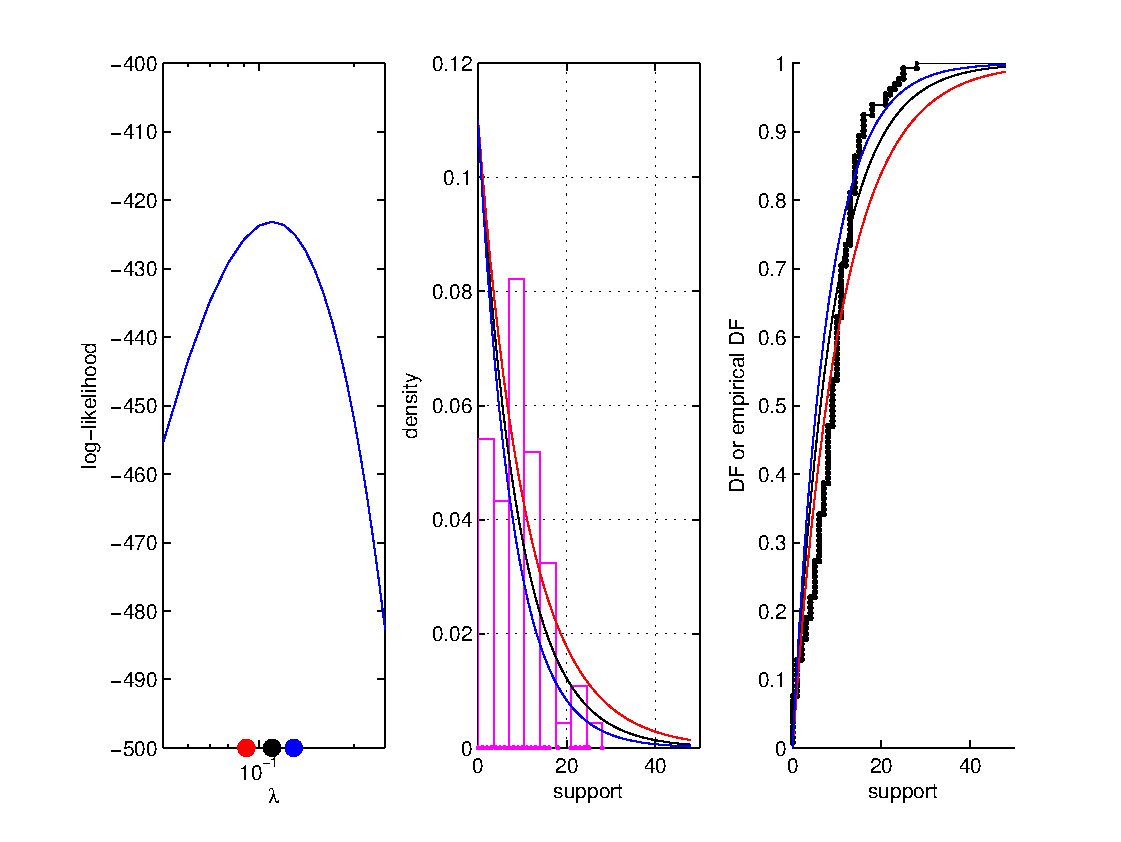
\includegraphics[width=6.5in]{figures/ExponentialMLECIOrbiter}}
\end{figure}

\begin{labwork}[Maximum likelihood estimation for Orbiter bus-stop]\label{LW:ExponentialMLECIOrbiter}
The above analysis was undertaken with the following M-file:
\VrbMf[label=ExponentialMLECIOrbiter.m]{scripts/ExponentialMLECIOrbiter.m}
A call to the script generates \hyperref[F:ExponentialMLECIOrbiter]{Figure~\ref*{F:ExponentialMLECIOrbiter}} and the following output of the sample mean, MLE, sample size, standard error and the $95\%$ confidence interval.  
\begin{VrbM}
>> ExponentialMLECIOrbiter
SampleMean =    9.0758
MLE =    0.1102
n =   132
StdErr =    0.0096
MLE95CI =    0.0914    0.1290
\end{VrbM}
\end{labwork}

\begin{labwork} [Maximum likelihood estimation for your bus-stop]\label{LW:IDSeededBusStopMLECI}
Recall \hyperref[LW:Next7Buses]{labwork~\ref*{LW:Next7Buses}} where you modeled the arrival of buses using $\exponential(\lambda^*=0.1)$ distributed inter-arrival time with a mean of $1/\lambda^*=10$ minutes.  Using the data of these seven inter-arrival times at your ID-seeded bus stop and pretending that you do not know the true $\lambda^*$, report (1) the ML estimate of $\lambda^*$, (2) $95\%$ confidence interval for it and (3) whether the true value $\lambda^*=1/10$ is engulfed by your confidence interval.  
\end{labwork}

\section{Delta Method}\label{S:DeltaMethod}
A more general estimation problem of interest concerns some function of the parameter $\theta \in \BB{\Theta}$, say $g(\theta)=\psi:\BB{\Theta} \to \BB{\Psi}$.  So, $g(\theta)=\psi$ is a function from the parameter space $\BB{\Theta}$ to $\BB{\Psi}$.  Thus, we are not only interested in estimating the fixed and possibly unknown $\theta^* \in \BB{\Theta}$ using the ML estimator $\widehat{\Theta}_n$ and its ML estimate $\widehat{\theta}_n$, but also in estimating $\psi^* = g(\theta^*) \in \BB{\Psi}$ via an estimator $\widehat{\Psi}_n$ and its estimate $\widehat{\psi}_n$.  We exploit the equivariance property of the ML estimator $\widehat{\Theta}_n$ of $\theta^*$ and use the Delta method to find the following analytically:
\begin{enumerate}
\item The ML estimator of $\psi^*=g(\theta^*) \in \BB{\Psi}$ is 
$$\boxed{\widehat{\Psi}_n = g(\widehat{\Theta}_n)}$$ 
and its point estimate is 
$$\boxed{\widehat{\psi}_n=g(\widehat{\theta}_n)}$$
\item Suppose $g(\theta)=\psi:\BB{\Theta} \to \BB{\Psi}$ is {\bf any} smooth function of $\theta$, i.e.~$g$ is differentiable, and $g'(\theta) := \frac{\partial}{\partial \theta}g(\theta) \neq 0$.  Then, the distribution of the ML estimator $\widehat{\Psi}_n$ is asymptotically $\normal(\psi^*, {\widehat{\mathsf{se}}_n(\widehat{\Psi}_n)}^2)$, i.e.:
\[
\boxed{
\frac{\widehat{\Psi}_n - \psi^*}{\widehat{\mathsf{se}}_n(\widehat{\Psi}_n)} \rightsquigarrow
\normal(0,1)
}
\]
where the standard error $\widehat{\mathsf{se}}_n(\widehat{\Psi}_n)$ of the ML estimator $\widehat{\Psi}_n$ of the unknown quantity $\psi^* \in \BB{\Psi}$ can be obtained from the standard error $\widehat{\mathsf{se}}_n(\widehat{\Theta}_n)$ of the ML estimator $\widehat{\Theta}_n$ of the parameter $\theta^* \in \BB{\Theta}$, as follows:
\[
\boxed{
\widehat{\mathsf{se}}_n(\widehat{\Psi}_n) = |g'(\widehat{\theta}_n)| \widehat{\mathsf{se}}_n(\widehat{\Theta}_n)
}
\]
\item Using $\normal(\psi^*, {\widehat{\mathsf{se}}_n(\widehat{\Psi}_n)}^2)$, we can construct the estimate of an approximate Normal-based $1-\alpha$ confidence interval for $\psi^* \in \BB{\Psi}$:
\[
\boxed{
C_n  =[\underline{C}_n, \overline{C}_n]= \widehat{\psi}_n \pm z_{\alpha/2} {\widehat{\mathsf{se}}_n(\widehat{\psi}_n)}
}
\]
\end{enumerate}

Let us do an example next.
\begin{example}
Let $X_1,X_2,\ldots,X_n \overset{IID}{\sim} \bernoulli(\theta^*)$.  Let $\psi=g(\theta)=\log(\theta/(1-\theta))$.  Suppose we are interested in producing a point estimate and confidence interval for $\psi^*=g(\theta^*)$.  We can use the Delta method as follows: 

First, the estimated standard error of the ML estimator of $\theta^*$, as shown in \hyperref[EX:BernoulliFisherInfo]{Example~\ref*{EX:BernoulliFisherInfo}}, is
\[
\widehat{\mathsf{se}}_n(\widehat{\Theta}_n) = \sqrt{\frac{\widehat{\theta}_n (1-\widehat{\theta}_n)}{n}} \ .
\]
The ML estimator of $\psi^*$ is:
$$\widehat{\Psi}_n=\log(\widehat{\Theta}_n / (1-\widehat{\Theta}_n))$$ 
and the ML estimate of $\psi^*$ is:
$$\widehat{\psi}_n=\log(\widehat{\theta}_n / (1-\widehat{\theta}_n)) \ .$$
Since, $g'(\theta) = 1/(\theta (1-\theta))$, by the Delta method, the estimated standard error of the ML estimator of $\psi^*$ is:
\[
\widehat{\mathsf{se}}_n(\widehat{\Psi}_n) = |g'(\widehat{\theta}_n)| (\widehat{\mathsf{se}}_n(\widehat{\Theta}_n))
= \frac{1}{\widehat{\theta}_n (1-\widehat{\theta}_n)} \sqrt{\frac{\widehat{\theta}_n (1-\widehat{\theta}_n)}{n}}
= \frac{1}{\sqrt{n\widehat{\theta}_n (1-\widehat{\theta}_n)}}
= \frac{1}{\sqrt{n \overline{x}_n (1-\overline{x}_n)}} \ .
\]
An approximate $95\%$ confidence interval for $\psi^*=\log(\theta^*/(1-\theta^*))$ is:
\[
\widehat{\psi}_n \pm \frac{1.96}{\sqrt{n \widehat{\theta}_n (1-\widehat{\theta}_n)}}
= \log(\widehat{\theta}_n / (1-\widehat{\theta}_n)) \pm \frac{1.96}{\sqrt{n \widehat{\theta}_n (1-\widehat{\theta}_n)}}
= \log(\overline{x}_n / (1-\overline{x}_n)) \pm \frac{1.96}{\sqrt{n \overline{x}_n (1-\overline{x}_n)}} \ .
\]
\end{example}

\begin{example}[Delta Method for a $\normal$ Experiment]\label{EX:NormalDelta}
Let us try the Delta method on a continuous RV.  Let $X_1,X_2,\ldots,X_n \overset{IID}{\sim} \normal(\mu^*, {\sigma^*}^2)$.  Suppose that $\mu^*$ is known and $\sigma^*$ is unknown.  Let us derive the ML estimate $\widehat{\psi}_n$ of $\psi^* = \log(\sigma^*)$ and a $95\%$ confidence interval for it in 6 steps.

(1) First let us find the log-likelihood function $\ell(\sigma)$ 
\begin{flalign*}
\ell(\sigma) 
& := \log (L(\sigma)) := \log( L(x_1,x_2,\ldots,x_n; \sigma)) = \log \left( \prod_{i=1}^n f(x_i; \sigma) \right) = \sum_{i=1}^n \log \left( f(x_i; \sigma) \right) \\
& = \sum_{i=1}^n \log \left( \frac{1}{\sigma \sqrt{2 \pi}}
 \exp{\left( - \frac{1}{2 \sigma^2} (x_i-\mu)^2 \right)} \right) \quad \because \text{\scriptsize{$f(x_i;\sigma)$ in \eqref{E:Normalpdf} is pdf of $\normal(\mu,\sigma^2)$ RV with known $\mu$}} \\
 & =  \sum_{i=1}^n \left( \log \left( \frac{1}{\sigma \sqrt{2 \pi}} \right) +
 \log \left( \exp{\left( - \frac{1}{2 \sigma^2} (x_i-\mu)^2 \right)} \right) \right) \\
& =  \sum_{i=1}^n \log \left( \frac{1}{\sigma \sqrt{2 \pi}} \right) +
 \sum_{i=1}^n \left( - \frac{1}{2 \sigma^2} (x_i-\mu)^2 \right)
 = n \log \left( \frac{1}{\sigma \sqrt{2 \pi}} \right) +
\left( - \frac{1}{2 \sigma^2} \right) \sum_{i=1}^n (x_i-\mu)^2 \\
& = n \left( \log \left( \frac{1}{\sqrt{2 \pi}} \right) + \log \left( \frac{1}{\sigma} \right) \right) -
\left( \frac{1}{2 \sigma^2} \right) \sum_{i=1}^n (x_i-\mu)^2 \\
& = n \log \left({\sqrt{2 \pi}}^{-1} \right) + n \log \left( \sigma^{-1} \right)  -
\left( \frac{1}{2 \sigma^2} \right) \sum_{i=1}^n (x_i-\mu)^2 \\
& = - n \log \left({\sqrt{2 \pi}} \right) - n \log \left( \sigma \right)  -
\left( \frac{1}{2 \sigma^2} \right) \sum_{i=1}^n (x_i-\mu)^2 
\end{flalign*}
(2) Let us find its derivative with respect to the unknown parameter $\sigma$ next.
\begin{flalign*}
\frac{\partial}{\partial \sigma } \ell(\sigma) 
& :=
\frac{\partial}{\partial \sigma } \left( - n \log \left({\sqrt{2 \pi}} \right) - n \log \left( \sigma \right)  -
\left( \frac{1}{2 \sigma^2} \right) \sum_{i=1}^n (x_i-\mu)^2 \right) \\
& = \frac{\partial}{\partial \sigma } \left( - n \log \left({\sqrt{2 \pi}} \right) \right) 
-  \frac{\partial}{\partial \sigma } \left( n \log \left( \sigma \right) \right) 
-  \frac{\partial}{\partial \sigma } \left( \left( \frac{1}{2 \sigma^2} \right) \sum_{i=1}^n (x_i-\mu)^2 \right)  \\
& = 0 - n  \frac{\partial}{\partial \sigma } \left( \log(\sigma) \right) - \left( \frac{1}{2} \sum_{i=1}^n (x_i-\mu)^2 \right) \frac{\partial}{\partial \sigma } \left( \sigma^{-2} \right) \\
& = -n \sigma^{-1} - \left( \frac{1}{2} \sum_{i=1}^n (x_i-\mu)^2 \right) \left(-2  \sigma^{-3} \right)
 = -n \sigma^{-1} +  \sigma^{-3} \sum_{i=1}^n (x_i-\mu)^2
\end{flalign*}
(3) Now, let us set the derivative equal to $0$ and solve for $\sigma$.
\begin{flalign*}
0  =  -n \sigma^{-1} +  \sigma^{-3} \sum_{i=1}^n (x_i-\mu)^2 
& \iff n \sigma^{-1}   =   \sigma^{-3} \sum_{i=1}^n (x_i-\mu)^2 
 \iff n \sigma^{-1} \sigma^{+3}    =   \sum_{i=1}^n (x_i-\mu)^2 \\
& \iff n \sigma^{-1+3}    =   \sum_{i=1}^n (x_i-\mu)^2 
\iff n \sigma^{2}    =   \sum_{i=1}^n (x_i-\mu)^2 \\
& \iff \sigma^{2}    =  \left( \sum_{i=1}^n (x_i-\mu)^2 \right) / n
\iff \sigma = \sqrt{\sum_{i=1}^n(x_i-\mu)^2/n}
\end{flalign*}
Finally, we set the solution, i.e.~the maximiser of the concave-down log-likelihood function of $\sigma$ with a known and fixed $\mu^*$ as our ML estimate $\widehat{\sigma}_n=\sqrt{\sum_{i=1}^n(x_i-\mu^*)^2/n}$.  Analogously, the ML estimator of $\sigma^*$ is $\widehat{\Sigma}_n=\sqrt{\sum_{i=1}^n(X_i-\mu^*)^2/n}$.  Don't confuse $\Sigma$, the upper-case sigma, with $\sum_{i=1}^n \bigcirc_i $, the summation over some $\bigcirc_i$'s.  This is usually clear from the context.

(4) Next, let us get the estimated standard error $\widehat{se}_n$ for the estimator of $\sigma^*$ via Fisher Information.  The Log-likelihood function of $\sigma$, based on one sample from the $\normal(\mu, \sigma^2)$ RV with known $\mu$ is,
\[
\log f(x;\sigma) = \log \left( \frac{1}{\sigma \sqrt{2 \pi}}
 \exp{\left( - \frac{1}{2 \sigma^2} (x-\mu)^2 \right)} \right)
 = - \log \left({\sqrt{2 \pi}} \right) - \log \left( \sigma \right)  -
\left( \frac{1}{2 \sigma^2} \right)  (x-\mu)^2 \\
\]
Therefore, in much the same way as in part (2) earlier,
\begin{flalign*}
\frac{\partial^2 \log f(x;\sigma)}{\partial^2 \sigma} 
& := \frac{\partial}{\partial \sigma} 
\left( 
\frac{\partial}{\partial \sigma} 
\left(  
- \log \left({\sqrt{2 \pi}} \right) - \log \left( \sigma \right)  - \left( \frac{1}{2 \sigma^2} \right)  
(x-\mu)^2 \right) \right) \\
& = \frac{\partial}{\partial \sigma} 
\left( -\sigma^{-1}  +  \sigma^{-3} 
(x-\mu)^2 \right) 
 = \sigma^{-2}  -3  \sigma^{-4} (x-\mu)^2 
\end{flalign*}
Now, we compute the Fisher Information of one sample as an expectation of the continuous RV $X$ over $\Xz = (-\infty,\infty)$ with density $f(x;\sigma)$,
\begin{flalign*}
I_1(\sigma) 
& = - \int_{x \in \Xz = (-\infty,\infty)} \left( \frac{\partial^2 \log f(x;\sigma)}{\partial^2 \lambda} \right) f(x;\sigma) \ dx
 =  - \int_{-\infty}^{\infty} \left( \sigma^{-2}  -3  \sigma^{-4} (x-\mu)^2  \right) f(x;\sigma) \ dx \\
 &=   \int_{-\infty}^{\infty} -\sigma^{-2}  f(x;\sigma) \ dx +  \int_{-\infty}^{\infty} 3  \sigma^{-4} (x-\mu)^2  f(x;\sigma) \ dx \\
& =  -\sigma^{-2} \int_{-\infty}^{\infty} f(x;\sigma) \ dx + 3  \sigma^{-4} \int_{-\infty}^{\infty} (x- \mu)^2  f(x;\sigma) \ dx \\
& =  -\sigma^{-2}  + 3  \sigma^{-4} \sigma^2  \qquad \qquad \because \sigma^2 = \V(X) = \E(X- \E(X))^2 = \int_{-\infty}^{\infty} (x- \mu)^2  f(x;\sigma) \ dx \\
& =  -\sigma^{-2}  + 3  \sigma^{-4+2} =  -\sigma^{-2}  + 3  \sigma^{-2}  = 2 \sigma^{-2}  
\end{flalign*}
Therefore, the estimated standard error of the estimator of the unknown $\sigma^*$ is
\[
\widehat{\mathsf{se}}_n(\widehat{\Sigma}_n) = \frac{1}{\sqrt{I_n(\widehat{\sigma}_n)}} = \frac{1}{\sqrt{n I_1 (\widehat{\sigma}_n)}}
=  \frac{1}{\sqrt{n 2 \sigma^{-2}}} =  \frac{\sigma}{\sqrt{2 n}}  \ .
\]
(5) Given that $\psi=g(\sigma)=\log(\sigma)$, we derive the estimated standard error of $\psi^*=\log(\sigma^*)$ via the Delta method as follows:
\[
\widehat{\mathsf{se}}_n(\widehat{\Psi}_n) = |g'(\sigma)| \widehat{\mathsf{se}}_n(\widehat{\Sigma}_n) = \left| \frac{\partial}{\partial \sigma} \log(\sigma) \right|  \frac{\sigma}{\sqrt{2 n}} 
= \frac{1}{\sigma} \frac{\sigma}{\sqrt{2 n}} = \frac{1}{\sqrt{2 n}} \ .
\]
(6) Finally, the $95\%$ confidence interval for $\psi^*$ is $\widehat{\psi}_n \pm 1.96 \widehat{\mathsf{se}}_n(\widehat{\Psi}_n) = \log(\widehat{\sigma}_n) \pm 1.96 \frac{1}{\sqrt{2 n}} $.
\end{example}


%In summary, there are three basic experimental situations to bear in mind, when estimating confidence sets from data.  We already saw the first two situations.
%\begin{enumerate}
%\item
%{\bf Variance of point estimator, $\mathbf {\mathsf{se}}_n^2$, is known {\em a priori}:}\\
%This was the case in Example \hyperref[EX:CLTPoisson]{\ref*{EX:CLTPoisson}} as well as Example 6.8 of Ang \& Tang.  In such a case, we may can obtain the {\bf exact} confidence interval directly via:
%\[
%C_n := [\underline{C}_{\, n}, \overline{C}_{\, n}]
%= [\widehat{\Theta}_n - z_{\alpha/2} {\mathsf{se}}_n, \widehat{\Theta}_n + z_{\alpha/2} {\mathsf{se}}_n] \ .
%\]
%\item
%{\bf Variance of point estimator, $\mathbf {\mathsf{se}}_n^2$, is unknown but we have numerous samples, say $n \geq 30$:}\\
%In this case, we may use the asymptotically valid approximation $\widehat{\mathsf{se}}_n$ for ${\mathsf{se}}_n$ to compute the confidence interval.
%\[
%C_n := [\underline{C}_{\, n}, \overline{C}_{\, n}]
%= [\widehat{\Theta}_n - z_{\alpha/2} \widehat{\mathsf{se}}_n, \widehat{\Theta}_n + z_{\alpha/2} \widehat{\mathsf{se}}_n]
%\]
%\item
%{\bf Variance of point estimator, $\mathbf {\mathsf{se}}_n^2$, is unknown and we have few samples, say $n < 30$:}
%In this case, the asymptotically valid approximation may not hold any longer and we see how one can handle this situation in \hyperref[S:SmallSamples]{\ref*{S:SmallSamples}}.
%\end{enumerate}

%\section{One-sided Confidence Intervals}
%So far, we have only considered two-sided confidence intervals, i.e.~both end-points of the confidence interval are random variables, actually estimators.  In some decision situations, we may want to fix one of these end-points to some value and only estimate the other one.

%notes...

%\section{Small Samples, Measurement Theory and Student's $t$-Distrubution}\label{S:SmallSamples}

%See notes in class.

%Student's $\mathfrak{t}$-distribution

%determining sample size

%measurement theory
\clearpage
}

\chapter{Maximum Likelihood Estimation for Multiparameter Models}\label{S:MultiParamEst}

\section{Introduction}\label{S:MultiParamEstIntro}
When two or more parameters index a statistical experiment we want to estimate the vector-valued parameter $\theta^* := (\theta^*_1,\ldots,\theta^*_k)$.
Here we will find the maximum likelihood estimates of vector-valued parameters.  

The maximum likelihood estimator (MLE) of a possibly unknown but fixed parameter  $\theta^* := (\theta^*_1,\ldots,\theta^*_k)$  in a multi-parametric experiment, i.e.~$\theta^* \in \BB{\Theta} \subset \Rz^k$ with $1 < k < \infty$ is defined analogously to \hyperref[D:LklFn]{Definition~\ref*{D:MLE}} with the exception that we allow the parameter to be a vector.  We take an excursion in multi-dimensional optimisation before finding the MLE of a parametric experiment involving two parameters.

 \section{Practical Excursion in Multi-dimensional Optimisation}\label{S:PracticalMultiDimOptimization}
The basic idea involves multi-dimensional iterations that attempt to converge on a local maximum close to the starting vector $\theta^{(0)} \in \BB{\Theta}$ (our initial guess).  We can employ {\sc Matlab}'s built-in function {\tt fminsearch} to find the MLE of vector-valued parameters such as in the $\lognormal$ model with two parameters, i.e.~$\theta=(\lambda,\zeta) \in \BB{\Theta} \subset \Rz^2$.  The  function {\tt fminsearch} is similar to {\tt fminbnd} except that it handles a given function of many variables, and the user specifies a starting vector $\theta^{(0)}$ rather than a starting interval.  Thus, {\tt fminsearch} tries to return a vector $\theta^{(*)}$ that is a local minimiser of, $-\log(L(x_1,x_2,\ldots,x_n; \theta)$, the negative log-likelihood function of the vector-valued parameter $\theta$, near this starting vector $\theta^{(0)}$.  
We illustrate the use of {\tt fminsearch} on a more challenging target called the Levy density:

{\scriptsize
\begin{equation}\label{E:LevyDensity}
f(x,y)   =  \exp \left(-\frac{1}{50} \left( \left( \sum_{i=1}^5 {i \cos{((i-1)x+i)} } \right) \left( \sum_{j=1}^5 {j \cos{((j+1)y+j)} } \right)+ (x + 1.42513 )^2 + (y + 0.80032)^2\right) \right)
\end{equation}
}

\begin{figure}[htpb]
\caption{Plot of Levy density as a function of the parameter $(x,y) \in [-10,10]^2$ scripted in \hyperref[Mf:LevyDensityPlot]{Labwork \ref*{Mf:LevyDensityPlot}}.\label {F:LevyDensityPlot}}
\begin{center}
\makebox{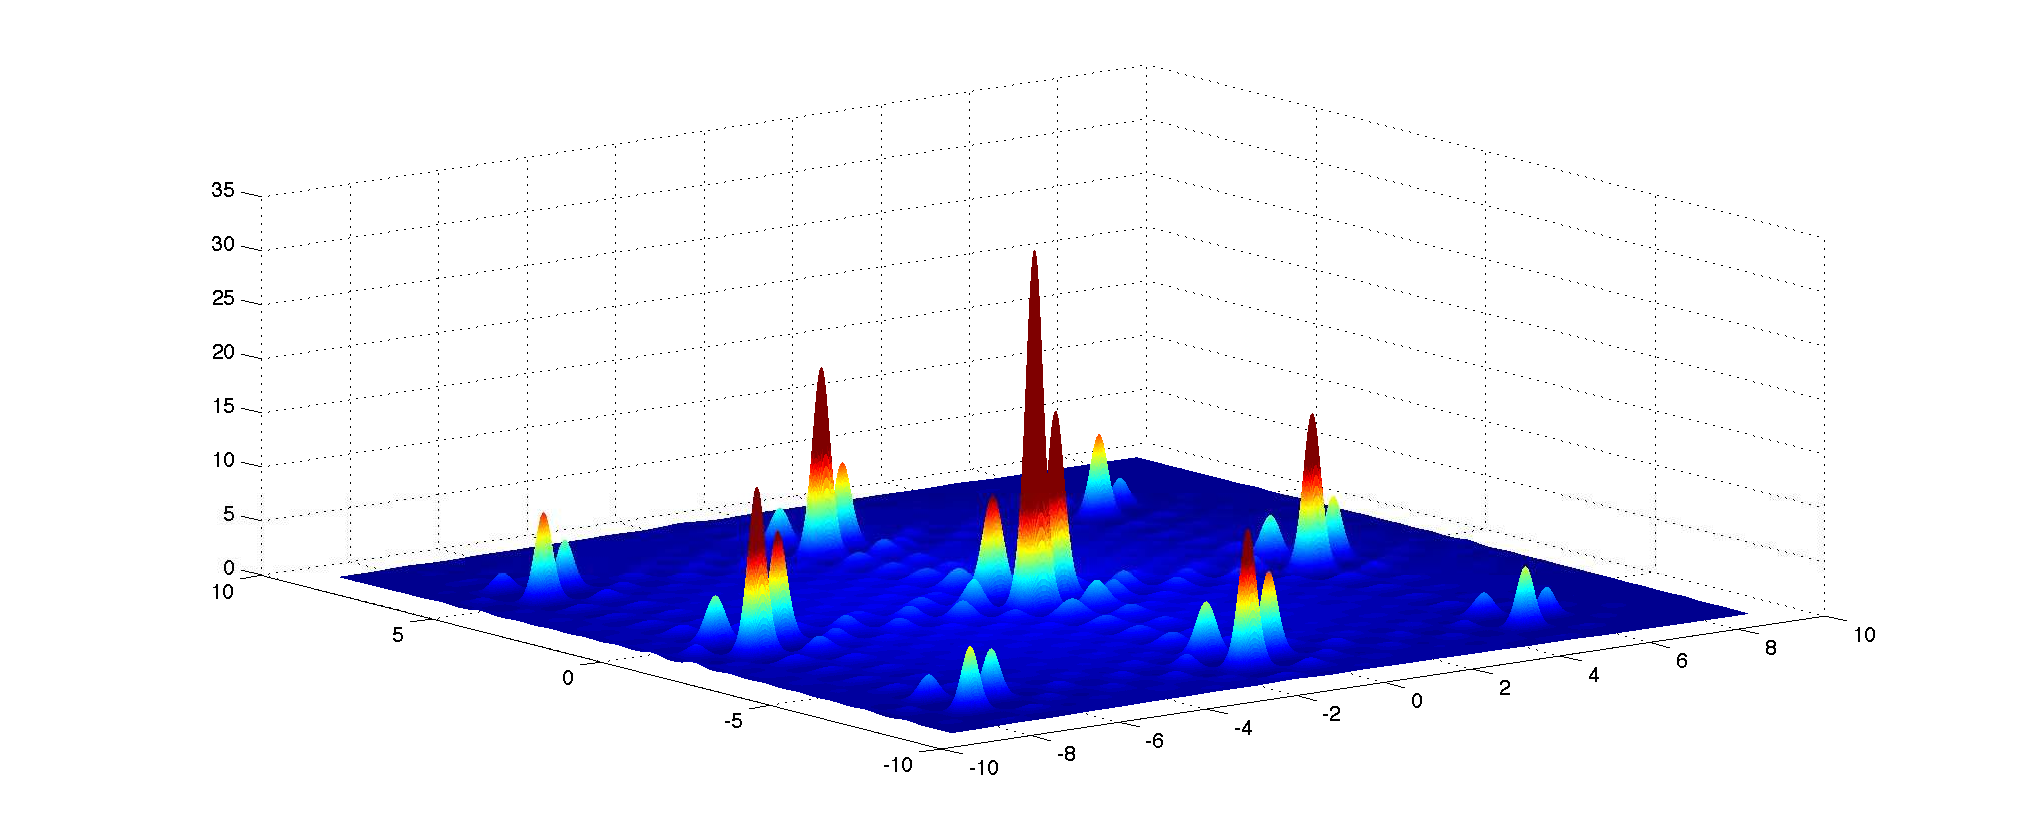
\includegraphics[width=6.750in]{figures/LevyDensityT50}}
\end{center}
\end{figure}

{\tt fminsearch} uses the simplex search method [Nelder, J.A., and Mead, R.~1965, Computer Journal, vol.~7, p.~308-313].  For an animation of the method and more details, please visit \href{http://en.wikipedia.org/wiki/Nelder-Mead_method}{\url{http://en.wikipedia.org/wiki/Nelder-Mead_method}}.  
%For a more recent treatment see Lagarias, J.C., J. A. Reeds, M. H. Wright, and P. E. Wright, {\em Convergence Properties of the Nelder-Mead Simplex Method in Low Dimensions}, SIAM Journal of Optimisation, Vol. 9 Number 1, pp. 112-147, 1998.  
An advantage of the method is that it does not use numerical (finite differencing) or analytical (closed-form expressions) gradients but relies on a direct search method.  Briefly, the simplex algorithm tries to ``tumble and shrink'' a simplex towards the local valley of the function to be minimised.  If $k$ is the dimension of the parameter space or domain of the function to be optimised, a $k$-dimensional simplex is specified by its $k+1$ distinct vertices each of dimension $k$.  Thus, a simplex is a triangle in a two-dimensional space and a pyramid in a three-dimensional space. At each iteration of the algorithm: 
\begin{enumerate}
\item A new point inside or nearby the current simplex is proposed.
\item The function's value at the newly proposed point is compared with its values at the vertices of the simplex. 
\item One of the vertices is typically replaced by the proposed point, giving rise to a new simplex. 
\item The first three steps are repeated until the diameter of the simplex is less than the specified tolerance.  
\end{enumerate}

A major limitation of {\tt fminsearch}, as demonstrated with the Levy target (encoded in \hyperref[Mf:NegLevyDensity]{Labwork~\ref*{Mf:NegLevyDensity}}) is that it  can only give local solutions.  The {\bf global maximiser} of the Levy function $f(x,y)$ is $(-1.3069, -1.4249)$ and the {\bf global maximum} is $f (-1.3069, -1.4249)=33.8775$ For instance, if we start the search close to, say $(x^{(0)},y^{(0)})=(-1.3,-1.4)$, as shown below, then the simplex algorithm converges as desired to the solution $(-1.3068, -1.4249)$.
\begin{VrbM}
>> [params, fvalue, exitflag, output] = fminsearch('NegLevyDensity',[-1.3 -1.4],options)
params =   -1.3068   -1.4249
fvalue =  -33.8775
exitflag =     1
output = 
    iterations: 24
     funcCount: 46
     algorithm: 'Nelder-Mead simplex direct search'
       message: [1x194 char]
\end{VrbM}
However, if we start the search further away, say $(x^{(0)},y^{(0)})=(1.3,1.4)$, as shown below, then the algorithm converges to the {\bf local maximiser} $(1.1627,1.3093)$ with a {\bf local maximum} value of $f(1.1627,1.3093)=0.9632$, which is clearly smaller than the global maximum of $33.8775$.  
\begin{VrbM}
>> [params, fvalue, exitflag, output] = fminsearch('NegLevyDensity',[1.3 1.4],options)
params = 1.1627    1.3093
fvalue = -0.9632
exitflag = 1
output = 
   iterations: 29
     funcCount: 57
     algorithm: 'Nelder-Mead simplex direct search'
       message: [1x194 char]
\end{VrbM}
Therefore, we have to be extremely careful when using point-valued, iterative,  local optimisation algorithms, implemented in floating-point arithmetic to find the global maximum.  Other examples of such algorithms include:
\begin{itemize}
\item {\bf Conjugate Gradient Method}:\\ \href{http://en.wikipedia.org/wiki/Conjugate_gradient_method}{\url{http://en.wikipedia.org/wiki/Conjugate_gradient_method}}
\item {\bf Broyden-Fletcher-Goldfarb-Shanno (BFGS) method}:\\ \href{http://en.wikipedia.org/wiki/BFGS_method}{\url{http://en.wikipedia.org/wiki/BFGS_method}}
\item {\bf Simulated Annealing}:\\ \href{http://en.wikipedia.org/wiki/Simulated_annealing}{\url{http://en.wikipedia.org/wiki/Simulated_annealing}}
\end{itemize}
In general, we have no guarantee that the output of such local optimisation routines will indeed be the global optimum.  In practice, you can start the search at several distinct starting points and choose the best local maximum from the lot.

\begin{figure}[hbpt]
\caption{Plot of the ``well-behaved'' (uni-modal and non-spiky) $\log(L((x_1,x_2,\ldots,x_{100});\lambda,\zeta))$, based on $100$ samples $(x_1,x_2,\ldots,x_{100})$ drawn from the $\lognormal(\lambda^*=10.36,\zeta^*=0.26)$ as per \hyperref[Mf:LogNormalLogLklPlot]{Labwork \ref*{Mf:LogNormalLogLklPlot}}.\label {F:LogNormalLogLklPlot}}
\begin{center}
\makebox{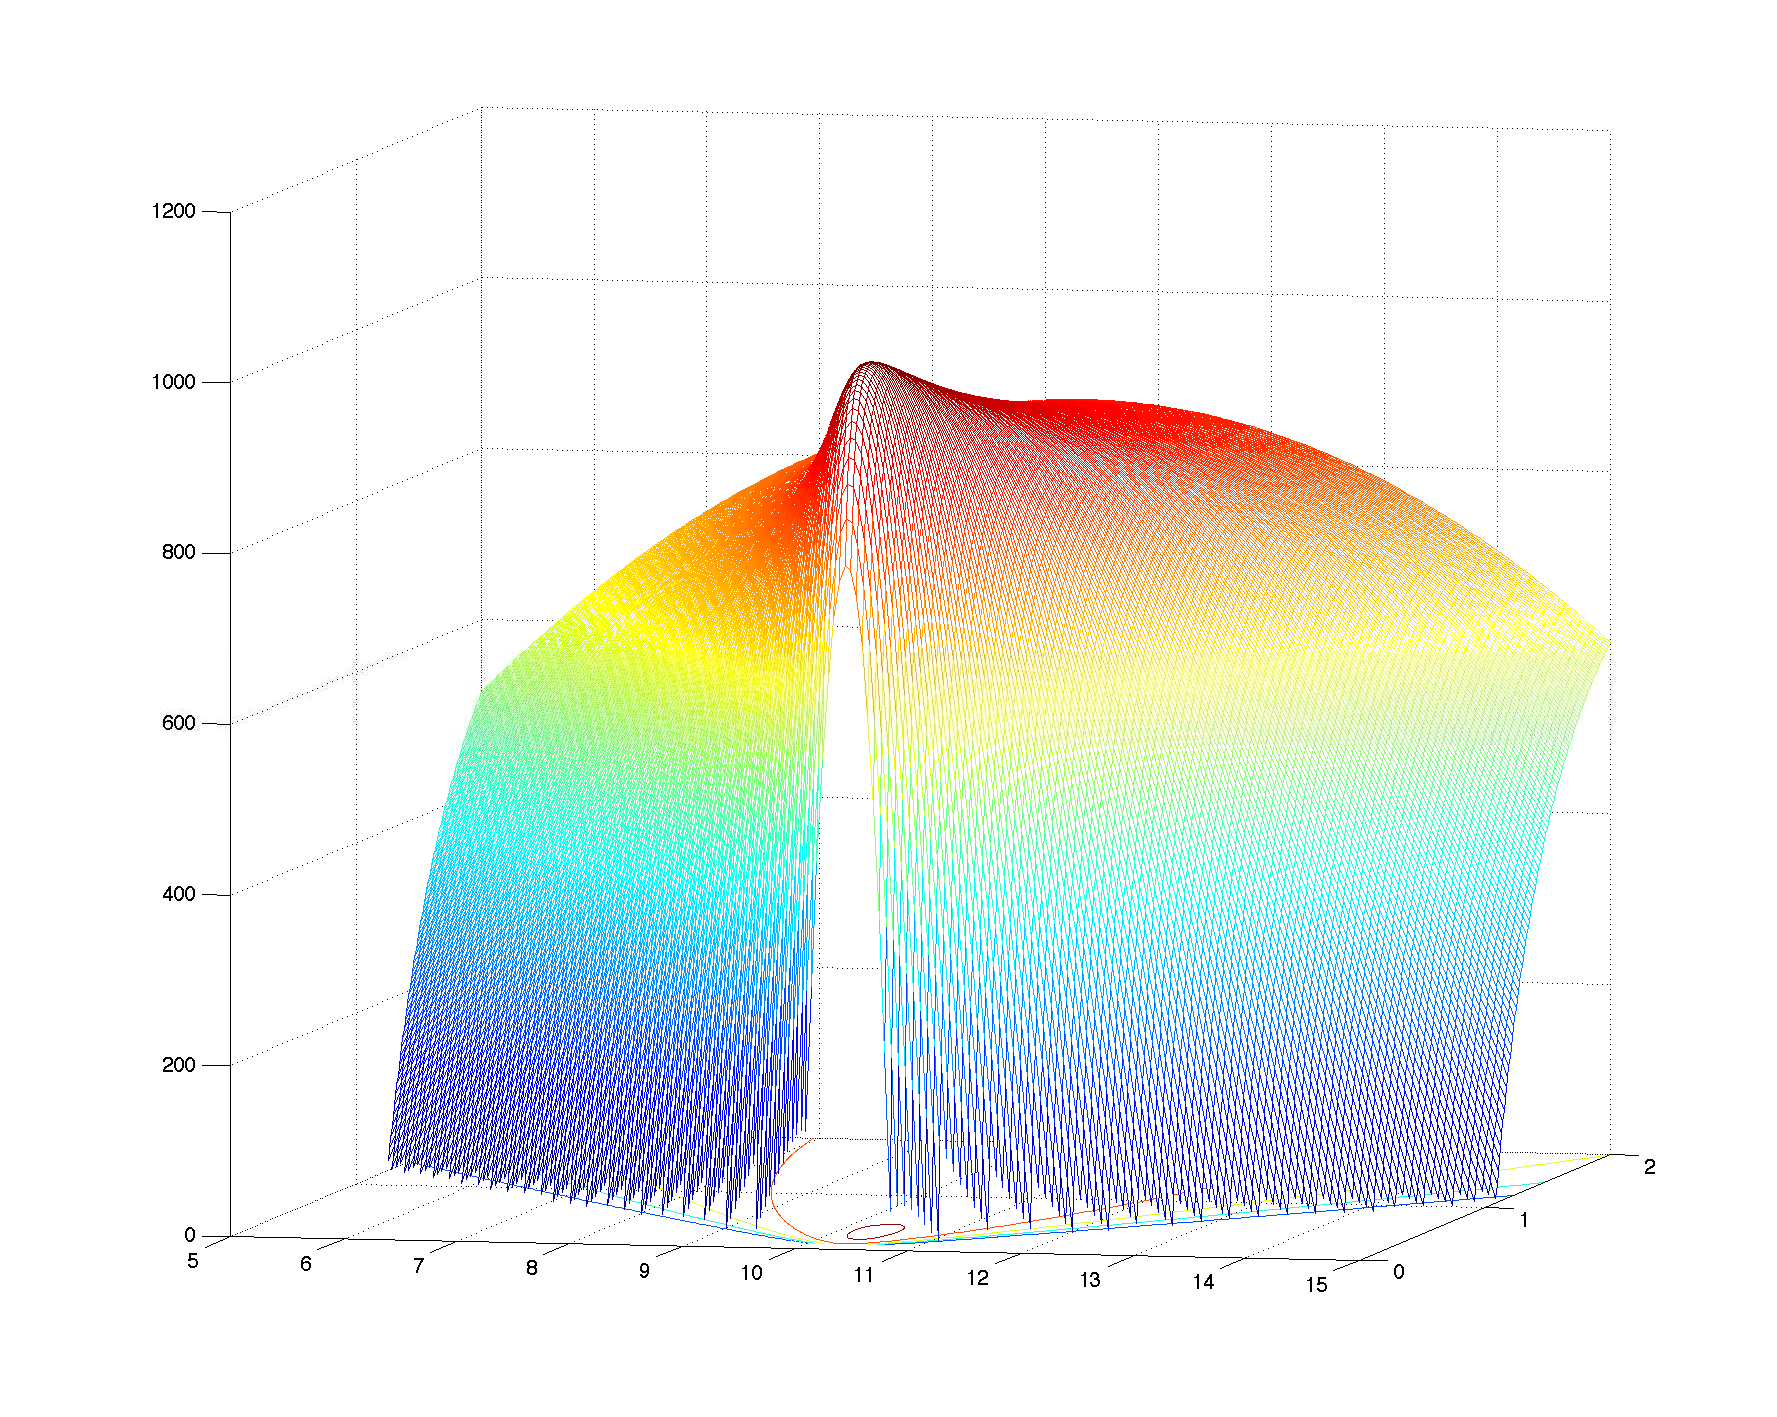
\includegraphics[width=4.0in]{figures/LogNormalLogLklPlot}}
\end{center}
\end{figure}

When the target function is ``well-behaved,'' i.e.~uni-modal or single-peaked and not too spiky, the optimisation routine can be expected to perform well.  Log-likelihood functions are often well-behaved.  Let us generate $100$ samples from an RV $C\sim \lognormal(\lambda^*=10.36, \zeta^*=0.26)$ by exponentiating the samples from the $\normal(10.36,0.26^2)$ RV, and then compute the corresponding MMEs and MLEs for parameters $(\lambda,\zeta)$ using the formulae in \hyperref[T:MMEMLE]{Table~\ref*{T:MMEMLE}}.
\begin{VrbM}
>> rand('twister',001); % set the fundamental sampler
>> % draw 100 samples from the Lognormal(10.36,0.26) RV
>> Cs = exp(arrayfun(@(u)(Sample1NormalByNewRap(u,10.36,0.26^2)),rand(1,100))); 
>> MLElambdahat = mean(log(Cs)) % maximum likelihood estimate of lambda 
MLElambdahat =   10.3397
>> MLEzetahat = sqrt(mean( (log(Cs)-MLElambdahat) .^ 2)) % max. lkl. estimate of zeta
MLEzetahat =    0.2744
>> MMEzetaahat = sqrt(log(var(Cs)/(mean(Cs)^2) + 1)) % moment estimate of zeta
MMEzetaahat =    0.2624
>> MMElambdahat = log(mean(Cs))-(0.5*MMEzetaahat^2) % moment estimate of lambda
MMElambdahat =   10.3417
\end{VrbM}
Let us try to apply the simplex algorithm to find the MLE numerically.  We first encode the negative log-likelihood function of the parameters $(\lambda,\zeta) \in (0,\infty)^2$ for the given data $x$, as follows: 
{\VrbMf[label=NegLogNormalLogLkl.m]{scripts/NegLogNormalLogLkl.m}}
Here is how we can call {\tt fminsearch} and find the MLE after the re-transformation. 
\begin{VrbM}
>> [params, fvalue, exitflag, output] = ...
fminsearch(@(params)(NegLogNormalLogLkl(Cs,params)),[log(5), log(1)])
params =    2.3360   -1.2931
fvalue =  -1.0214e+03
exitflag =     1
output = 
    iterations: 74
     funcCount: 131
     algorithm: 'Nelder-Mead simplex direct search'
       message: [1x194 char]
>> % But we want exp(params) since we defined lambda and zeta as exp(params)
exp(params)
ans =   10.3397    0.2744
\end{VrbM}
Note that the MLEs $(\widehat{\lambda}_{100},\widehat{\zeta}_{100}) = (10.3397,0.2744)$ from $74$ iterations or ``tumbles'' of the `Nelder-Mead simplex (triangle)' and the MLEs agree well with the direct evaluations {\tt MLElambdahat} and {\tt MLEzetahat} based on the formulae in \hyperref[T:MMEMLE]{Table~\ref*{T:MMEMLE}}.

%%\newpage
%\begin{labwork}
%Recall \hyperref[LW:lognormal]{labwork~\ref*{LW:lognormal}} where you simulated $1000$ samples directly from the RV $C$ (in part 3.).  Pretend that you do not know the true parameters used in this particular simulation from RV $C$ and do the following:
%\begin{enumerate}
%\item Store the first 10, the first 100 and all 1000 samples in data arrays named {\tt x10}, {\tt x100} and {\tt x1000} [Please don't do this manually!].
%\item Report the MLE of the two parameters for each of the three sub-arrays of data, namely {\tt x10}, {\tt x100} and {\tt x1000}, i.e.~report the six point estimates: $\widehat{\lambda}_{10},\widehat{\zeta}_{10},\widehat{\lambda}_{100},\widehat{\zeta}_{100},\widehat{\lambda}_{1000},\widehat{\zeta}_{1000}$.
%\item Report the MME of the two parameters for each of the three sub-arrays of data, namely {\tt x10}, {\tt x100} and {\tt x1000}, i.e.~report the six point estimates: $\widehat{\lambda}_{10},\widehat{\zeta}_{10},\widehat{\lambda}_{100},\widehat{\zeta}_{100},\widehat{\lambda}_{1000},\widehat{\zeta}_{1000}$.
%\item Discuss in a short paragraph what you can deduce from the two sets of point estimates.  Explain how the maximum likelihood (ML) and method of moments (MM) estimates of the parameters are related to the true parameters used in the simulation as the sample size increases in powers of $10$. 
%\item {\bf There is no credit for this part}: Try to use {\tt fminsearch} to numerically find the MLE for your data and make a 2D-plot of the log-likelihood function being maximised.
%\end{enumerate} 
%\end{labwork}

\subsubsection*{Summarizing Table of Point Estimators}
Using the sample mean $\overline{X}_n$ and sample standard deviation $S_n$ defined in \eqref{E:SampleMeanRV} and \eqref{E:SampleStdDevRV}, respectively, we summarise the two point estimators of the parameters of some common distributions below.  For some cases, the MLE is the same as the MME (method of moments) and can be solved analytically.
\begin{center}
\begin{table}[htbp]
\caption{Summary of the Method of Moment Estimator (MME) and the Maximum Likelihood Estimator (MLE) for some IID Experiments. \label{T:MMEMLE}}
\begin{tabular}{l | r | r}
\hline
Statistical Experiment & MLE & MME \\ \hline
$X_1,X_2,\ldots,X_n \overset{IID}{\sim} \bernoulli(\theta)$ & $\widehat{\theta}=\overline{X}_n$ & same as MLE \\ \hline
$X_1,X_2,\ldots,X_n \overset{IID}{\sim} \exponential(\lambda)$ & $\widehat{\lambda}={1}/{\overline{X}_n} $ & same as MLE \\ \hline
$X_1,X_2,\ldots,X_n \overset{IID}{\sim} \normal(\mu,\sigma^2)$ & $\widehat{\mu}=\overline{X}_n, \widehat{\sigma} = \sqrt{\frac{n-1}{n}S^2_n} $ & $\widehat{\mu}=\overline{X}_n, \widehat{\sigma} = S_n $ \\ \hline
$X_1,X_2,\ldots,X_n \overset{IID}{\sim} \lognormal(\lambda,\zeta)$ & $\widehat{\lambda}=\frac{1}{n}{\sum_{i=1}^n \log(X_i)} $ & $\widehat{\lambda} = \log(\overline{X}_n) - \frac{1}{2} {\widehat{\zeta}} \ ^2$ \\ %\\
 & $\widehat{\zeta} = \sqrt{\frac{1}{n} \sum_{i=1}^n{(\log(X_i)-\widehat{\lambda})^2}} $ & $\widehat{\zeta} = \sqrt{\log \left({S_n^2}/{\overline{X}_n^2} +1 \right)}$ \\
\hline
\end{tabular}
\end{table}
\end{center}

\section{Confidence Sets for Multiparameter Models}\label{S:ConfSetsMultiParamModels}
We will extend the Fisher Information and Delta method to models with more than one parameter:
\[
X_1,X_2,\ldots,X_n \overset{IID}{\sim} f(x;\theta^*), \qquad \theta^* := (\theta_1^*, \theta_2^*, \ldots, \theta_k^*) \in \BB{\Theta} \subset \Rz^k  \ .
\]
Let, the ML estimator of the fixed and possibly unknown vector-valued parameter $\theta^*$ be:
\[
\widehat{\Theta}_n := \left( \widehat{\Theta}_{1,n}, \widehat{\Theta}_{2,n}, \ldots, \widehat{\Theta}_{k,n} \right), \qquad  \widehat{\Theta}_n := \widehat{\Theta}_n(X_1,X_2,\ldots,X_n) : \Xz_n \to \BB{\Theta}
\]
and the ML estimate based on $n$ observations $x_1,x_2,\ldots,x_n$ be:
\[
\widehat{\theta}_n := \left( \widehat{\theta}_{1,n}, \widehat{\theta}_{2,n}, \ldots, \widehat{\theta}_{k,n} \right), \qquad  \widehat{\theta}_n := \widehat{\theta}_n(x_1,x_2,\ldots,x_n) \in \BB{\Theta} \ .
\]
Let the log-likelihood function and its Hessian matrix $H = (H_{i,j})_{i,j=1,2,\ldots,k}$ of partial derivatives be:
\[
\ell_n(\theta) := \ell_n(\theta_1,\theta_2,\ldots,\theta_k) := \sum_{i=1}^n \log(f(x_i; (\theta_1,\theta_2,\ldots,\theta_k))), \qquad
H_{i,j} := \frac{\partial}{\partial \theta_i} \frac{\partial}{\partial \theta_j} \ell_n(\theta_1,\theta_2,\ldots,\theta_k) \ ,
\]
respectively, provided the log-likelihood function is sufficiently smooth.
\begin{definition}[Fisher Information Matrix]  The Fisher Information matrix is:
\begin{equation}\label{E:FisherInfoMat}
I_n(\theta) := I_n(\theta_1,\theta_2,\ldots,\theta_k) =
-
\begin{bmatrix}
\E_{\theta}(H_{1,1}) & \E_{\theta}(H_{1,2}) & \cdots & \E_{\theta}(H_{1,k}) \\
\E_{\theta}(H_{2,1}) & \E_{\theta}(H_{2,2}) & \cdots & \E_{\theta}(H_{2,k}) \\
\vdots & \vdots & \ddots & \vdots \\
\E_{\theta}(H_{k,1}) & \E_{\theta}(H_{k,2}) & \cdots & \E_{\theta}(H_{k,k})
\end{bmatrix}
\end{equation}
and its matrix inverse is denoted by $I_n^{-1}(\theta)$.
\end{definition}
\begin{prop}[Asymptotic Normality of MLE in Multiparameter Models]
Let 
$$X_1,X_2,\ldots,X_n \overset{IID}{\sim} f(x_1;\theta_1^*,\theta_2^*,\ldots,\theta_k^*), \qquad \theta^*=(\theta_1^*,\theta_2^*,\ldots,\theta_k^*)\in \BB{\Theta}\subset \Rz^k \ ,$$
for some fixed and possibly unknown $\theta^* \in \BB{\Theta}\subset \Rz^k$.  Then, under appropriate regularity conditions:
\[
{\widehat{\Theta}_n} := \left( \widehat{\Theta}_{1,n}, \widehat{\Theta}_{2,n}, \ldots, \widehat{\Theta}_{k,n} \right) \rightsquigarrow \normal(\theta^*,I_n^{-1})
\]
In other words, the vector-valued estimator $\widehat{\Theta}_n$ converges in distribution to the multivariate $\normal$ distribution centred at the unknown parameter $\theta^*$ with the variance-covariance matrix given by inverse Fisher Information matrix $I_n^{-1}$.  Furthermore, let $I_n^{-1}(j,j)$ denote the $j^{\text{th}}$ diagonal entry of $I_n^{-1}$.  In this case:
% and let $$\widehat{\mathsf{se}}_n ( \widehat{\Theta}_{j,n}) = \sqrt{ I_n^{-1}(j,j)}$$  be the standard error of the estimator of $\theta_j^*$
\[
\frac{\widehat{\Theta}_{j,n} - \theta^*_j}{\sqrt{I_n^{-1}(j,j)}} \rightsquigarrow \normal(0,1)
\]
and the approximate covariance of $\widehat{\Theta}_{i,n}$ and $\widehat{\Theta}_{j,n}$ is:
\[
{\sf Cov}({\Theta}_{i,n},{\Theta}_{j,n}) \approxeq I_n^{-1}(i,j) \ .
\]
\end{prop}
Now, let us look at a way of obtaining ML estimates and confidence sets for functions of $\theta$.  Suppose the real-valued function $g(\theta)=\psi:\BB{\Theta} \to \BB{\Psi}$ maps points in the $k$-dimensional parameter space $\BB{\Theta} \subset \Rz^k$ to points in $\BB{\Psi} \subset \Rz$.  Let the gradient of $g$ be
\[
\bigtriangledown g(\theta)
:=
\bigtriangledown g (\theta_1,\theta_2,\ldots,\theta_k)
=
\begin{pmatrix}
\frac{\partial} {\partial \theta_1}{g(\theta_1,\theta_2,\ldots,\theta_k)} \\
\frac{\partial} {\partial \theta_2}{g(\theta_1,\theta_2,\ldots,\theta_k)} \\
\vdots \\
\frac{\partial} {\partial \theta_k}{g(\theta_1,\theta_2,\ldots,\theta_k)} \\
\end{pmatrix} \ .
\]
\begin{prop}[Multiparameter Delta Method]
Suppose:
\begin{enumerate}
\item $X_1,X_2,\ldots,X_n \overset{IID}{\sim} f(x_1;\theta_1^*,\theta_2^*,\ldots,\theta_k^*), \qquad \theta^*=(\theta_1^*,\theta_2^*,\ldots,\theta_k^*)\in \BB{\Theta}\subset \Rz^k$,
\item Let  $\widehat{\Theta}_n$ be a ML estimator of $\theta^* \in \BB{\Theta}$ and let $\widehat{\theta}_n$ be its ML estimate, and
\item Let $g(\theta)=\psi:\BB{\Theta} \to \BB{\Psi} \subset \Rz$ be a smooth function such that $\bigtriangledown g(\widehat{\theta}_n) \neq 0$.
\end{enumerate}
Then: 
\begin{enumerate}
\item $\widehat{\Psi}_n = g(\widehat{\Theta}_n)$ is the ML estimator and  $\widehat{\psi}_n = g(\widehat{\theta}_n)$ is the ML estimate of of $\psi^*=g(\theta^*) \in \BB{\Psi}$,
\item The standard error of the ML estimator of $\psi^*$ is:
$$\widehat{\sf{se}}_n(\widehat{\Psi}_n) = \sqrt{ \left( \bigtriangledown g(\widehat{\theta}_n) \right)^T I_n^{-1}(\widehat{\theta}_n) \left( \bigtriangledown g(\widehat{\theta}_n) \right)}, $$
\item The ML estimator of $\psi^*$ is asymptotically normal, i.e.:
$$\frac{\widehat{\Psi}_n - \psi^*}{\widehat{\sf{se}}_n(\widehat{\Psi}_n)} \rightsquigarrow \normal(0,1) \  ,$$
\item And a $1-\alpha$ confidence interval for $\psi^*$ is:
\[
\widehat{\psi}_n \pm z_{\alpha/2} {\widehat{\sf{se}}_n(\widehat{\Psi}_n)} 
\]
\end{enumerate}
\end{prop}
Let us put the theory to practice in the problem of estimating the coefficient of variation from samples of size $n$ from an RV.
\begin{example}[Estimating the Coefficient of Variation of a $\normal(\mu^*,{\sigma^*}^2)$ RV]\label{EX:CoeffOfVarForBivNormal}
Let 
$$
\psi^* = g(\mu^*,\sigma^*)=\sigma^*/\mu^*, \qquad X_1,X_2,\ldots,X_n \overset{IID}{\sim} \normal(\mu^*,{\sigma^*}^2) \ .
$$ 
We do not know the fixed parameters $(\mu^*,\sigma^*)$ and are interested in estimating the coefficient of variation $\psi^*$ based on $n$ IID samples $x_1,x_2,\ldots,x_n$.  We have already seen that the ML estimates of $\mu^*$ and $\sigma^*$ are:
\[
\widehat{\mu}_n =  \overline{x}_n := \frac{1}{n}\sum_{i=1}^n x_i,  \qquad 
\widehat{\sigma}_n = s_n := \sqrt{\frac{1}{n} \sum_{i=1}^n (x_i-\widehat{\mu}_n)^2} \ .
\]
Thus, the ML estimate of $\psi^*=\sigma^*/ \mu^*$ is:
\[
\widehat{\psi}_n =  \frac {\widehat{\sigma}_n}{\widehat{\mu}_n} = \frac {s_n}{\overline{x}_n}
\] 
We can now derive the standard error of the ML estimator $\widehat{\Psi}_n$ by first computing $I_n(\mu,\sigma)$, $I_n^{-1}(\mu,\sigma)$, and $\bigtriangledown g(\mu,\sigma)$.  A careful computation shows that:
\[
I_n(\mu,\sigma) = 
\begin{bmatrix}
\frac{n}{\sigma^2} & 0\\
0 & \frac{2n}{\sigma^2}
\end{bmatrix},
\qquad \qquad
I_n^{-1}(\mu,\sigma) = 
\frac{1}{n}
\begin{bmatrix}
{\sigma^2} & 0\\
0 & \frac{\sigma^2}{2}
\end{bmatrix},
\qquad \qquad
\bigtriangledown g(\mu,\sigma) =
\begin{pmatrix}
-\frac{\sigma}{\mu^2} \\
\frac{1}{\mu}
\end{pmatrix} \ .
\]
Therefore, the standard error of interest is:
\[
\widehat{\sf{se}}_n(\widehat{\Psi}_n) = \sqrt{ \left( \bigtriangledown g(\widehat{\theta}_n) \right)^T I_n^{-1}(\widehat{\theta}_n) \left( \bigtriangledown g(\widehat{\theta}_n) \right)} = 
\frac{1}{\sqrt{n}} \sqrt{\frac{1}{\widehat{\mu}_n^4} + \frac{\widehat{\sigma}_n^2}{2 \widehat{\mu}_n^2}}
\]
and the $95\%$ confidence interval for the unknown coefficient of variation $\psi^*$ is:
\[
\widehat{\psi}_n \pm z_{\alpha/2} {\widehat{\sf{se}}_n(\widehat{\Psi}_n)}  = 
\frac{s_n}{\overline{x}_n} \pm z_{\alpha/2} \left( \frac{1}{\sqrt{n}} \sqrt{\frac{1}{\widehat{\mu}_n^4} + \frac{\widehat{\sigma}_n^2}{2 \widehat{\mu}_n^2}} \right)
\]
\end{example}

Let us get our hands dirty in the machine with Labwork~\ref{LW:CoeffOfVarForBivNormal} next.
\begin{labwork} [Computing the coefficient of variation of a $\normal(\mu^*,{\sigma^*}^2)$ RV]\label{LW:CoeffOfVarForBivNormal}
Let us apply these results to $n=100$ simulated samples from $\normal(100,10^2)$ as follows.
{\VrbMf[label=CoeffOfVarNormal.m]{scripts/CoeffOfVarNormal.m}}
\begin{VrbM}
>> CoeffOfVarNormal
Muhat =  100.3117
Sigmahat =   10.9800
Psihat =    0.1095
Sehat =    0.0077
ConfInt95 =    0.0943    0.1246
\end{VrbM}
\end{labwork}


%\newpage

%\section{Exercises}\label{Exs:onRV}

%\begin{ExerciseList}

%\end{ExerciseList}
%\newpage
